
\documentclass[12pt]{report}
% \documentclass[journal]{IEEEtran}

\usepackage{cite}
\usepackage{amsmath,amssymb,amsfonts}
\usepackage{algorithmic}
\usepackage{graphicx}
\usepackage{textcomp}
\usepackage{bm}
\usepackage{upgreek}

\usepackage[retainorgcmds]{IEEEtrantools}

\usepackage[nottoc]{tocbibind}


\linespread{1.3}


\title{Bayesian Learning using a Dirichlet Prior for Regression and Classification}
\author{Paul Rademacher}
%\date{}


%\graphicspath{ {C:/Users/Paul/Documents/PhD/Dissertation/Documentation/Figures/} }
\graphicspath{ {../Figures/} }


\DeclareMathOperator*{\argmin}{arg\,min}
\DeclareMathOperator*{\argmax}{arg\,max}

\DeclareMathOperator{\xrm}{\mathrm{x}}
\DeclareMathOperator{\Xrm}{\mathrm{X}}
\DeclareMathOperator{\yrm}{\mathrm{y}}
\DeclareMathOperator{\Yrm}{\mathrm{Y}}
\DeclareMathOperator{\Drm}{\mathrm{D}}
\DeclareMathOperator{\nrm}{\mathrm{n}}
\DeclareMathOperator{\nbarrm}{\bar{\mathrm{n}}}
\DeclareMathOperator{\zrm}{\mathrm{z}}

\DeclareMathOperator{\Prm}{\mathrm{P}}
\DeclareMathOperator{\prm}{\mathrm{p}}
\DeclareMathOperator{\Erm}{\mathrm{E}}
\DeclareMathOperator{\Crm}{\mathrm{C}}

\DeclareMathOperator{\Xcal}{\mathcal{X}}
\DeclareMathOperator{\Ycal}{\mathcal{Y}}
\DeclareMathOperator{\Dcal}{\mathcal{D}}
\DeclareMathOperator{\Ncal}{\mathcal{N}}
\DeclareMathOperator{\Zcal}{\mathcal{Z}}
\DeclareMathOperator{\Hcal}{\mathcal{H}}
\DeclareMathOperator{\Fcal}{\mathcal{F}}
\DeclareMathOperator{\Rcal}{\mathcal{R}}
\DeclareMathOperator{\Mcal}{\mathcal{M}}
\DeclareMathOperator{\Scal}{\mathcal{S}}
\DeclareMathOperator{\Pcal}{\mathcal{P}}

\DeclareMathOperator{\Rbb}{\mathbb{R}}
\DeclareMathOperator{\Nbb}{\mathbb{N}}
\DeclareMathOperator{\Zbb}{\mathbb{Z}}

\DeclareMathOperator{\Dir}{\mathrm{Dir}}
\DeclareMathOperator{\DM}{\mathrm{DM}}
\DeclareMathOperator{\Mult}{\mathrm{Mult}}
\DeclareMathOperator{\DP}{\mathrm{DP}}









\begin{document}

\maketitle
\tableofcontents

\chapter{Introduction}


PGR: bibliography

Theo: (mult moments), DP agg, Dir moments

Bishop: (dir eq), dir posterior, moments, mode

Ferguson: (agg Dir), agg DP - via theo, DP posterior, moments

Gershman: agg DP - ref ferg, discrete draws

Johnson GET PDF: mult moments, (mult agg, DM agg, DM moments)

Add Theo-PR???




\section{Background}

PGR: complete rework

This report details a Bayesian perspective on stastical learning theory for when both the observations and unobserved quantities are jointly distributed according to an unknown probability function. While the validity of Bayesian methods for statistical signal processing and machine learning has long been contended, the author believes it to be a justified approach that does not necessarily imply that the distribution model is `random'; rather, it simply reflects the desire of the user to formulate risk as a weighted sum of learner performance across the space of distributions. 

The success or failure of Bayesian learning methods hinge on how well the prior knowledge imparted by the designer matches reality. The prior distribution over the set of probability mass functions (PMF) used reflects the users confidence that different PMF's are responsible for generating the observed/unobserved random variables. If a highly subjective prior is chosen that strongly weights the actual PMF generating the data, low risk learning functions are possible even with limited training data; however, if the prior is poorly selected, a good solution will never be achieved. Conversely, an objective prior that treats the different PMF's equally will always be able to adapt will enough training data; if data is limited, however, the learning function may not deliver the required performance.

This work assumes that the prior distribution is Dirichlet. The class of Dirichlet probability density functions (PDF) have the desirable properties of full support over the set of possible PMF's and a tractable posterior distribution for independently and identically distributed data \cite{ferguson}. Furthermore, control of the Dirichlet parameters can enable both objective and subjective prior knowledge. Special cases including the uniform prior will be given specific attention.

After introducing the problem and discussing the relevant data probability distributions, the Bayesian framework will be applied to two of the most common loss functions in machine learning: the squared error loss function (common for regression), and the 0-1 loss function (common for classification). Optimal estimators/classifiers and their corresponding minimum risk will be presented for different Dirichlet prior distributions. Specific attention will be given to various asymptotic cases to show the differing performance for objective and subjective Dirichlet priors.




\section{Notation}

PGR: notation check for figures. use Ycal for plot theta indexing

PGR: use f opt symbols in figure titles/colorbars

PGR: bold vector format? center dot usage???

PGR: suppress arguments where sensible? eg Pd = theta

PGR: check notation throughout for expectation/variance operators

PGR: define special PDF functions in intro/distsecs?

PGR: use Pcal throughout


This section details the mathematical notation and typesetting conventions used throughout. Note that many variable scalars and functions including $x$, $y$, $g$, etc. are repeatedly redefined and reused to avoid introducing an excessive volume of symbols; unless explicitly stated, none of these variable definitions will hold in subsequent sections.



\subsection*{Sets and Function Arguments}

Sets will typically be typeset with a calligraphic font, such as $\Xcal$. Exceptions include common number sets such as the real numbers, which are typeset using blackboard bold $\Rbb$. Function spaces such as the set of functions $\Xcal \to \Ycal$ are compactly represented as $\Ycal^{\Xcal}$.

Various mappings will be defined for which the domain and/or the range are function spaces. The set of functions $\Xcal \to \Ycal$ is denoted $\Ycal^{\Xcal}$. For a mapping $g : \Zcal \to \Ycal^{\Xcal}$, the argument notation $g(z) \in \Ycal^{\Xcal}$ denotes a function, while $g(x;z) \in \Ycal$ is a specific value from that function. Semicolons are used to distinguish between the different groups of arguments. A set of finite sequences $\{1,\ldots,N\} \to \Scal$ will be represented as $\Scal^N$ for brevity.

The convention adopted for natural numbers is $\Nbb = \{1,2,\ldots\}$; the set of non-negative integers is denoted $\Zbb_{\geq 0} = \Nbb \cup \{0\}$. The set of positive real numbers $\Rbb^+$ excludes zero, while non-negative real numbers are represented as $\Rbb_{\geq 0} = \Rbb^+ \cup \{0\}$. The cardinality of countably infinite sets, including the set of natural numbers, is denoted $\aleph_0 = |\Nbb|$; the cardinality of uncountable sets such as $\Rbb$ is at least $\aleph_1$.

Numerous probability distribution functions will be defined over different domains. As such, for a given set $\Xcal$, define a set function $\Pcal$ which outputs the set of distributions $\Pcal(\Xcal)$. If $\Xcal$ is countable, the set is defined as $\Pcal(\Xcal) = \left\{ p \in {\Rbb_{\geq 0}}^{\Xcal}: \sum_{x \in \Xcal} p(x) = 1 \right\}$; if $\Xcal$ is a Euclidean space, the set is defined as $\Pcal(\Xcal) = \left\{ p \in {\Rbb_{\geq 0}}^{\Xcal}: \int_{\Xcal} p(x) \mathrm{d}x = 1 \right\}$.

PGR: aleph reference?

PGR: ref Rudin for range?



\subsection*{Random variables and functions}

Random variables and functions are denoted with roman font (e.g. $\xrm$), while specific values are denoted with italics (e.g. $x$). 

Consider a random function $\xrm \in \Xcal$. If $\Xcal$ is countable, either finite with $|\Xcal| \in \Nbb$ or countably infinite with $|\Xcal| = \aleph_0$, then $\xrm$ is a discrete random function and is characterized by a probability mass function (PMF) \cite {papoulis}, denoted $\Prm_{\xrm} \in \Pcal(\Xcal)$. If $\Xcal$ is a Euclidean space and is thus uncountable with $|\Xcal| \geq \aleph_1$, it is characterized by a probability density function (PDF) $\prm_{\xrm} \in \Pcal(\Xcal)$.

PGR: explicit PMF/PDF formula with P of events?

For notational simplicity, probability distributions are occasionally represented as $\Prm(\xrm)$; in such instances, the formal notation can be recovered by replacing the distribution with $\Prm_{\xrm}(x)$ and all instances of the roman symbol $\xrm$ with the italic symbol $x$. 

Consider $\xrm$ conditioned on another RV $\zrm \in \Zcal$. The conditional distribution is represented as $\Prm_{\xrm | \zrm} \in \Pcal(\Xcal)^{\Zcal}$, where the range of the function is a PMF over $\Xcal$. The arguments are notated as $\Prm_{\xrm | \zrm}(x|z)$ to separate the unobserved random values from the conditional ones. These distributions may be compactly represented as $\Prm(\xrm|\zrm)$. Often, the dependency on the conditional variable $\zrm$ will not be expressed in terms of a specific value $z$, but will be left in terms of the random variable itself; in this case, the more compact notation $\Prm_{\xrm | \zrm}(x)$ is used and the distribution is implied to be a function of $\zrm$.

Many distributions will be repeatedly used. Thus, special functions will be defined for the PDF's and PMF's of interest. For example, consider a Dirichlet distribution for a discrete random function $\xrm \in \Xcal$ with parameters $\alpha \in \mathcal{A}$; the PDF will be notated as $\Dir : \mathcal{A} \to \Pcal(\Xcal)$, where the range is the set of valid PDF's. More compactly, the notation $\xrm \sim \Dir(\alpha)$ implies that $\Prm_{\xrm} = \Dir(\cdot ; \alpha)$.




\subsection*{Expectation Operators}

The expectation operator $\Erm_{\xrm}$ of a discrete random function $\xrm$ operating on a scalar function $g$ is defined as
\begin{equation}
\Erm_{\xrm}\big[ g(\xrm) \big] = \sum_{x} \Prm_{\xrm}(x) g(x) \;,
\end{equation}
where the argument $g$ is an arbitrary scalar function of $\xrm$. Additionally, define the variance operator $\Crm_{\xrm}$ as
\begin{equation}
\Crm_{\xrm}\big[g(\xrm)\big] = \Erm_{\xrm} \bigg[ \Big( g(\xrm) - \Erm_{\xrm}\big[g(\xrm)\big] \Big)^2 \bigg] \;.
\end{equation}
When the function $g$ is the identity operator, such that $g(\xrm) = \xrm$, the mean and variance are represented by $\mu_{\xrm}$ and $\Sigma_{\xrm}$, respectively.

These operations can be performed with respect to a condtional distribution as well. In this case, the expectation operator is a function of the observed value of $\zrm$, such that
\begin{equation}
\Erm_{\xrm | \zrm}\big[ g(\xrm) \big](z) = \sum_{x} \Prm_{\xrm | \zrm}(x | z) g(x) \;.
\end{equation}
Similarly, the conditional variance is notated $\Crm_{\xrm | \zrm}\big[ g(\xrm) \big](z)$. When $g$ is the identity operator, the conditional mean and variance as represented by $\mu_{\xrm | \zrm}(z)$ and $\Sigma_{\xrm | \zrm}(z)$, respectively.

As with conditional distributions, it is common that an explicit value $z$ of the conditional RV will not be used, but rather the expectation will be left as a function of the random variable $\zrm$. In these cases, the argument is suppressed and the notation $\Erm_{\xrm | \zrm}\big[ g(\xrm) \big]$ implies the dependency on $\zrm$. This convention also holds for the conditional variance operator $\Crm_{\xrm | \zrm}$, as well as for the $\mu_{\xrm | \zrm}$ and $\Sigma_{\xrm | \zrm}$ operators.

If the range of $g$ is a function space, such that $g(\xrm)$ is itself a function over a set $\Ycal$, then the notation for these operators is expanded. Then, the output of the expectation operator is a function over $\Ycal$ represented by
\begin{equation}
\Erm_{\xrm}\big[ g(\xrm) \big](y) = \sum_{x} \Prm_{\xrm}(x) g(y;x) \;.
\end{equation}
Similarly, the covariance operator notation is modified and the output is a function over $\Ycal \times \Ycal$, 
\begin{IEEEeqnarray}{L}
\Crm_{\xrm}\big[g(\xrm)\big](y,y') \\
\quad = \Erm_{\xrm} \bigg[ \Big( g(y;\xrm) - \Erm_{\xrm}\big[g(y;\xrm)\big] \Big) \Big( g(y';\xrm) - \Erm_{\xrm}\big[g(y';\xrm)\big] \Big) \bigg] \nonumber \;.
\end{IEEEeqnarray}
As before, the notation is simplified when the function $g$ is the identity operator. If $\xrm$ is a random function over the set $\Ycal$, then the mean and covariance functions are $\mu_{\xrm}(y)$ and $\Sigma_{\xrm}(y,y')$. 

If the expectations are evaluated with respect to a conditional distribution $\Prm_{\xrm | \zrm}$, the additional argument for the observed random variable is added and the notation for the above operators extends to $\Erm_{\xrm|\zrm}\big[ g(\xrm) \big](y|z)$ and $\Crm_{\xrm|\zrm}\big[g(\xrm)\big](y,y'|z)$ for non-scalar outputs. When $g$ is the identity operation, the notation $\mu_{\xrm|\zrm}(y|z)$ and $\Sigma_{\xrm|\zrm}(y,y'|z)$ is used.

Again, it is common for the conditional RV $\zrm$ to be left as a random quantity instead of being explicitly defined. In such cases, the italic $z$ is dropped from the arguments and the formulae $\Erm_{\xrm|\zrm}\big[ g(\xrm) \big](y)$, $\Crm_{\xrm|\zrm}\big[g(\xrm)\big](y,y')$, $\mu_{\xrm|\zrm}(y)$, and $\Sigma_{\xrm|\zrm}(y,y')$ imply dependence on $\zrm$.

As for probability distributions, the subscript notation of these operators may be suppressed. In such cases, the expectations are to be performed with respect to the joint distribution of all random variables/functions (roman font) found in the argument. For example, $\Erm\big[f(\yrm,\xrm) | \zrm \big]$ compactly represents $\Erm_{\yrm,\xrm | \zrm}\big[f(\yrm,\xrm)\big]$.


\subsection*{Special Functions}

Certain specialized functions are detailed next. Both the Dirac and Kronecker delta functions will be used throughout. The Dirac delta function over a Euclidean domain $\Xcal$ is represented as $\delta(\cdot)$; it has support only at the point $x=0$ and satisfies
\begin{equation}
\int_{\Xcal} \delta(x) \mathrm{d}x = 1 \;.
\end{equation}
Consequently, it also satisfies
\begin{equation}
\int_{\Xcal} g(x) \delta(x) \mathrm{d}x = g(0) \;.
\end{equation}
Consider a countable set $\Xcal$; the Kronecker delta function has domain $\Xcal \times \Xcal$ and is defined as
\begin{equation}
\delta[x,x'] = \begin{cases} 1 & \mathrm{if} \ x = x', \\ 0 & \mathrm{if} \ x \neq x'.  \end{cases}
\end{equation}

PGR: reference Dirac/Kronecker?


The multinomial coefficient and multivariate beta function, which typically operate on sequences, are defined more generally for function inputs. The multinomial operator $\Mcal$ is used for functions $g : \Xcal \to \Zbb_{\geq 0}$ that map to non-negative integers from an arbitrary countable domain $\Xcal$. The output of the operator is
\begin{equation}
\Mcal(g) = \frac{\big( \sum_{x \in \Xcal} g(x) \big)!}{\prod_{x \in \Xcal} g(x)!} \;.
\end{equation}
Similarly, the beta function $\beta$ operates on functions $g : \Xcal \to \Rbb^+$ that map to positive real numbers from an arbitrary countable domain $\Xcal$, such that
\begin{equation}
\beta(g) = \frac{\prod_{x \in \Xcal} \Gamma\big( g(x) \big)}{\Gamma \left( \sum_{x \in \Xcal} g(x) \right)} \;.
\end{equation}
Note that the countable domains of the input functions may have an infinite number of elements. These functions will also be used to operate on a subset of a functions' domain $\Scal \subset \Xcal$ and its corresponding image. Set notation for a function is used to express the argument, so that $\Mcal\Big( \big\{ g(x) : x \in S \big\} \Big)$ and $\beta\Big( \big\{ g(x) : x \in S \big\} \Big)$.








\section{Objective}

Consider an observable random function $\xrm \in \Xcal$ and and unobservable random function $\yrm \in \Ycal$ which are jointly distributed according to an unknown probability distribution $\theta \in \Theta = \Pcal(\Ycal \times \Xcal)$, such that $\Prm_{\yrm,\xrm | \theta}(y,x | \theta) = \theta(y,x)$. Note that while the uppercase notation implies that $\Ycal \times \Xcal$ is countable, PDF's may be substituted for continuous random functions.

Also observed is a random sequence of $N$ samples from $\theta$, denoted $\Drm = ( \Yrm,\Xrm ) \in \Dcal = \{\Ycal \times \Xcal\}^N$. The $N$ data pairs are conditionally independent from one another and are identically distributed as $\Prm_{\Drm_n | \theta}(y,x | \theta) = \theta(y,x)$. The samples are also conditionally independent from $(\yrm,\xrm)$. Thus,
\begin{equation}
\Prm(\yrm,\xrm,\Drm | \theta) = \Prm(\yrm,\xrm | \theta) \prod_{n=1}^N \Prm\big( \Drm_n | \theta \big) \;.
\end{equation}

The objective is to design a decision function $f: \Dcal \mapsto \Hcal^{\Xcal}$ which produces a mapping from the space of the observed random variables to a decision space $\Hcal$. Define the function space $\Fcal = \left\{ {\Hcal^{\Xcal}} \right\}^{\Dcal}$, such that $f \in \Fcal$. The metric guiding the design is a loss function $\mathcal{L}: \Hcal \times \Ycal \mapsto \Rbb_{\geq 0}$ which penalizes the decision $h \in \Hcal$ based on the value of $\yrm$. 

Next, introduce the conditional expected loss, or conditional ``risk'',
\begin{equation} \label{eq:risk_cond}
\Rcal_{\Theta}(f ; \theta) = \Erm_{\Drm | \theta} \bigg[ \Erm_{\yrm,\xrm | \theta} \Big[ \mathcal{L}\big( f(\xrm;\Drm),\yrm \big) \Big] \bigg] \;.
\end{equation}
As the model $\theta$ is also unobserved, $\Rcal_{\Theta}: \Theta \mapsto \{ \Rbb_{\geq 0} \}^{\Fcal}$ is not yet a valid objective function for optimization. An operator must be chosen to remove the dependency on $\theta$ and form an objective function $\Fcal \mapsto \Rbb_{\geq 0}$.

One choice is to integrate over $\Theta$; to ensure a non-negative objective value, the weighting function should be non-negative. Also, as scaling the objective function will not change its minimizing argument, the weighting function can be constrained to integrate to one. These are the requirements for a valid probability density function (PDF); as such, the model $\theta$ is treated as a random process and a Bayesian approach can be adopted. 

Define the PDF $\prm(\theta): \Theta \mapsto \Rbb_{\geq 0}$. Now using Bayes rule, the risk can be formulated as
\begin{IEEEeqnarray}{rCl} \label{eq:risk}
\Rcal(f) & = & \Erm_{\theta}\big[ \Rcal_{\Theta}(f ; \theta) \big] \\
& = & \Erm_{\yrm,\xrm,\Drm}\big[ \mathcal{L}(f(\xrm;\Drm),\yrm) \big] \nonumber \\
& = & \Erm_{\xrm,\Drm}\Big[ \Erm_{\yrm | \xrm,\Drm} \big[ \mathcal{L}(f(\xrm;\Drm),\yrm) \big] \Big] \nonumber
\end{IEEEeqnarray}
and $\yrm$, $\xrm$, and $\Drm$ are jointly distributed random variables.

Finally, express the optimal learning function
\begin{equation} 
f^* = \argmin_{f \in \Fcal} \Rcal(f) \;.
\end{equation}
The learning functions are non-parametric and there are no restrictions on the set of achievable functions $\Fcal$. Thus, to minimize the risk, the decision expressed by the learning function $f$ for each observed value $\xrm$ and $\Drm$ is determined to be
\begin{equation} \label{eq:f_opt_xD}
f^*(\xrm;\Drm) = \argmin_{h \in \Hcal} \Erm_{\yrm | \xrm,\Drm}\big[ \mathcal{L}(h,\yrm) \big] \;.
\end{equation}
The optimal function achieves the minimum risk,
\begin{equation} \label{eq_risk_min}
\Rcal(f^*) = \Erm_{\xrm,\Drm} \left[ \min_{h \in \Hcal} \Erm_{\yrm | \xrm,\Drm}\big[ \mathcal{L}(h,\yrm) \big] \right] \;.
\end{equation}













\chapter{Finite Dirichlet Model}



This chapter demonstrates the optimal decision functions when the sets $\Ycal$ and $\Xcal$ are finite and the model $\theta$ is characterized by a Dirichlet distribution.


\section{Probability Distributions}

To determine the optimal decision function, the joint PMF $\Prm(\yrm,\xrm,\Drm)$ is required. Having already defined the distribution conditioned on the model $\theta$, all that remains is to select a PDF $\prm(\theta)$ reflecting the users prior knowledge. In this section, the Dirichlet distribution is used. The Dirichlet distribution possesses the desirable property of being the conjugate prior for the multinomial conditional distribution characterizing the data; as such, it will provide tractable forms for the model posterior distribution and lead to closed form expressions for the data conditional distribution used to design the decision function.

Other distributions of interest will be provided, such as the training data PMF $\Prm(\Drm)$ and the conditional distribution $\Prm(\yrm | \xrm,\Drm)$ used to form a decision given specific observations.



\subsection{Model PDF, $\prm(\theta)$} \label{sec:P_theta}

The Dirichlet PDF for the model $\theta \in \Theta$ is \cite{bishop}
\begin{IEEEeqnarray}{rCl}
\prm(\theta) & = & \beta(\alpha)^{-1} \prod_{y \in \Ycal} \prod_{x \in \Xcal} \theta(y,x)^{\alpha(y,x) - 1} \;,
\end{IEEEeqnarray}
where the user-selected PDF parameters $\alpha : \Ycal \times \Xcal \mapsto \Rbb^+$ are introduced and $\beta$ is the generalized beta function.

The parameter $\alpha$ controls around which models $\theta$ the PDF concentrates and how strongly. For convenience, introduce the concentration parameter $\alpha_0 \equiv \sum_{y \in \Ycal} \sum_{x \in \Xcal} \alpha(y,x)$. 

The first and second joint moments of the model are 
\begin{equation}
\mu_{\theta}(y,x) = \Erm\big[ \theta(y,x) \big] = \frac{\alpha(y,x)}{\alpha_0}
\end{equation}
and
\begin{IEEEeqnarray}{rCl}
\Erm\big[ \theta(y,x) \theta(y',x') \big] & = & \frac{\alpha(y,x) \alpha(y',x') + \alpha(y,x) \delta[y,y'] \delta[x,x']}{\alpha_0 (\alpha_0+1)} \;.
\end{IEEEeqnarray}
Observe that $\Prm(\yrm,\xrm) = \mu_{\theta}(\yrm,\xrm) = \alpha(\yrm,\xrm) / \alpha_0$. The covariance is
\begin{IEEEeqnarray}{rCl}
\Sigma_{\theta}(y,x,y',x') & = & \Erm\Big[ \big(\theta(y,x)-\mu_{\theta}(y,x)\big) \big(\theta(y',x')-\mu_{\theta}(y',x')\big) \Big] \\
& = & \frac{\mu_{\theta}(y,x) \delta[y,y'] \delta[x,x'] - \mu_{\theta}(y,x) \mu_{\theta}(y',x')}{\alpha_0+1} \nonumber \;.
\end{IEEEeqnarray}
Also, for $\alpha(y,x) > 1$, the maximizing value of the distribution is
\begin{equation}
\theta_\mathrm{max} = \argmax_{\theta \in \Theta} \prm(\theta) = \frac{\alpha - 1}{\alpha_0 - |\Ycal||\Xcal|} \;.
\end{equation}

Of specific interest is how $\prm(\theta)$ changes as the concentration parameter approaches its limiting values. For $\alpha_0 \to \infty$, the PDF concentrates at its mean, resulting in
\begin{IEEEeqnarray}{rCl}
\prm(\theta) & = & \delta\left( \theta - \frac{\alpha}{\alpha_0} \right) \;.
\end{IEEEeqnarray}
Conversely, for $\alpha_0 \to 0$, the PDF trends toward
\begin{IEEEeqnarray}{rCl}
\prm(\theta) & = & \sum_{y \in \Ycal} \sum_{x \in \Xcal} \frac{\alpha(y,x)}{\alpha_0} \delta\big( \theta - \delta[\cdot,y] \delta[\cdot,x] \big) \;,
\end{IEEEeqnarray}
which distributes its weight among the $|\Ycal| |\Xcal|$ models with an $\ell_0$ norm satisfying $\| \theta \|_0 = 1$. Note that the Dirac delta for these formulas is defined on the set $\Theta$, such that $\int_{\Theta} \delta(\theta) \mathrm{d}\theta = 1$.

PGR: formal proof for limiting PDFs???

These trends can be visualized with Figure \ref{fig:P_theta}. Note that for $\alpha_0=2.99$, $\alpha < 1$ and the PDF values at the boundaries of the domain trend to infinity; this is not captured by the plot color scale.

\begin{figure}
\centering
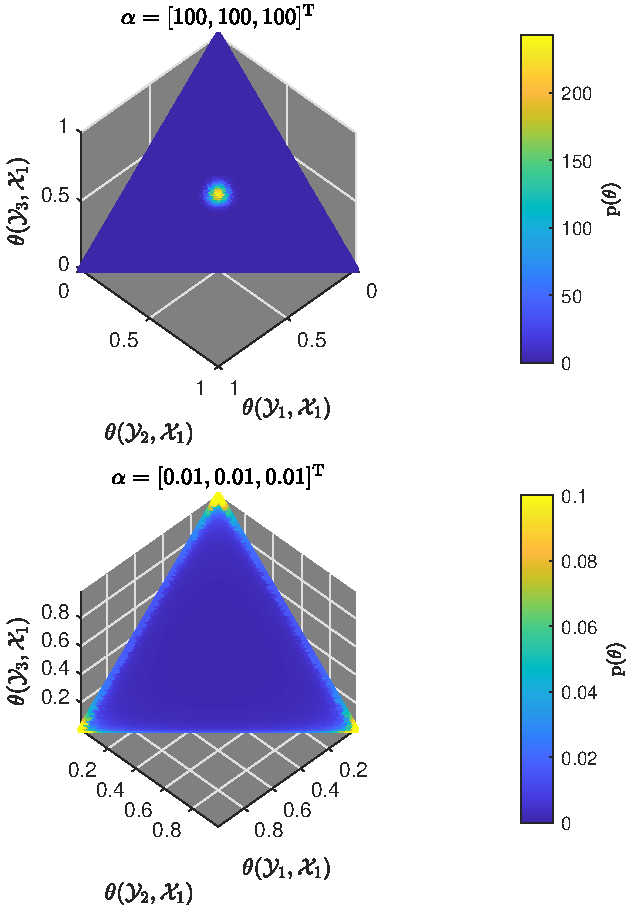
\includegraphics[scale=1.0]{P_theta.pdf}
\caption{Model prior PDF $\prm(\theta)$ for different concentrations $\alpha_0$}
\label{fig:P_theta}
\end{figure}





\paragraph{Uniform Prior}

When the parameterizing function is $\alpha(y,x) = 1$, the distribution becomes a uniform PDF over the simplex and is represented as
\begin{equation}
\prm(\theta) = \big( |\Ycal||\Xcal|-1 \big)! \cdot \delta \left( 1 - \sum_{y \in \Ycal} \sum_{x \in \Xcal}  \theta(y,x) \right) \;.
\end{equation}
Note that the concentration parameter is $\alpha_0 = |\Ycal||\Xcal|$ and $\Prm(\yrm,\xrm) = \big( |\Ycal||\Xcal| \big)^{-1}$ is also uniform. Figure \ref{fig:P_theta_uniform} shows the uniform distribution amplitude for $|\Ycal| = 3$, $|\Xcal| = 1$.

\begin{figure}
\centering
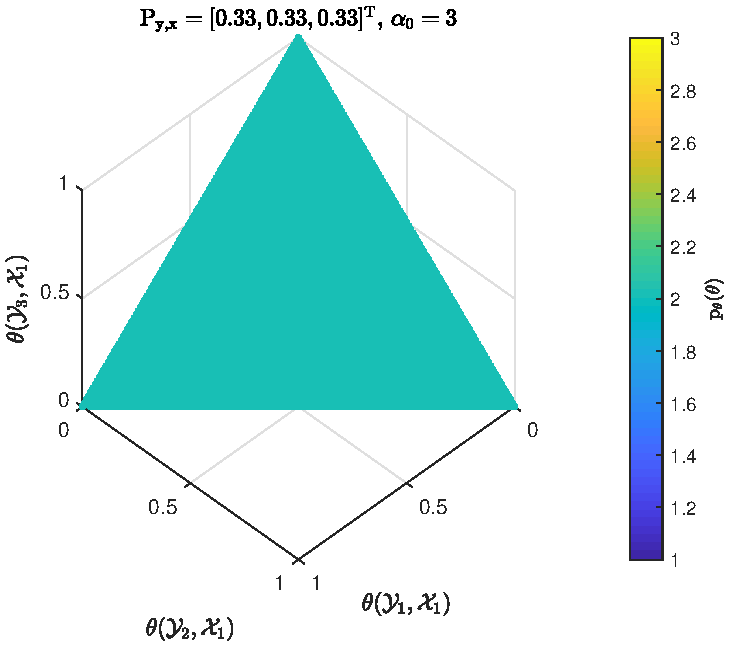
\includegraphics[scale=1.0]{P_theta_uniform.pdf}
\caption{Uniform model prior PDF, $|\Ycal| = 3$}
\label{fig:P_theta_uniform}
\end{figure}



\subsubsection{Aggregation Properties}

As $\xrm$ is observable and $\yrm$ is not, the marginal distribution $\theta'$ over the set $\Xcal$, defined as $\theta'(x) \equiv \sum_{y \in \Ycal} \theta(y,x)$, will also be of interest. By the aggregation property \cite{ferguson}, $\theta'$ is a Dirichlet random function parameterized by $\alpha'$, where $\alpha'(x) \equiv \sum_{y \in \Ycal} \alpha(y,x)$. Note that $\Prm(\xrm) = \alpha'(\xrm) / \alpha_0$ and $\Prm(\yrm|\xrm) = \alpha(\yrm,\xrm) / \alpha'(\xrm)$. 

Also of interest is the distribution of the model $\theta$ conditioned on its aggregation $\theta'$. As demonstrated in Appendix \ref{app:Dir_agg},
\begin{IEEEeqnarray}{rCl}
\prm(\theta | \theta') & = & \prod_{x \in \Xcal} \Bigg[ \frac{\theta'(x)^{1-|\Ycal|}}{\beta\big( \alpha(\cdot,x) \big)} \prod_{y \in \Ycal} \left(\frac{\theta(y,x)}{\theta'(x)}\right)^{\alpha(y,x)-1} \Bigg] \;,
\end{IEEEeqnarray}
which is defined for $\theta \in \left\{ {\Rbb_{\geq 0}}^{\Ycal \times \Xcal} : \sum_{y \in \Ycal} \theta(y,x) = \theta'(x), \quad \forall x \in \Xcal \right\}$. More interestingly, define $\tilde{\theta}(y;x) \equiv \theta(y,x) / \theta'(x)$ - it can be shown that the transformed random function conditioned on the aggregation is characterized by
\begin{IEEEeqnarray}{rCl}
\prm\big( \tilde{\theta} | \theta' \big) & = & \prod_{x \in \Xcal} \Bigg[ \beta\big( \alpha(\cdot,x) \big)^{-1} \prod_{y \in \Ycal} \tilde{\theta}(y;x)^{\alpha(y,x)-1} \Bigg] \\
& = & \prod_{x \in \Xcal} \Dir\Big( \tilde{\theta}(\cdot,x) ; \alpha(\cdot,x) \Big) \nonumber \;,
\end{IEEEeqnarray}
a product of Dirichlet distributions defined for $\tilde{\theta} \in \left\{ \tilde{\theta}(\cdot,x) \in \Pcal(\Ycal), \quad \forall x \in \Xcal \right\}$. As shown, the scaled functions $\tilde{\theta}(\cdot,x)$ are Dirichlet with parameterizing functions $\alpha(\cdot,x)$, independent of one another, and independent of the aggregation $\theta'$.








\subsection{Training Set PMF's, $\Prm(\Drm|\theta)$ and $\Prm(\Drm)$}

Next, the conditional distribution $\Prm(\Drm|\theta)$ will be used top determine the marginal PMF, $\Prm(\Drm)$; properties of both distributions will be discussed. 

The distribution of $\Drm$ conditioned on the model can be formulated as
\begin{IEEEeqnarray}{rCl}
\Prm\big( \Drm | \theta \big) & = & \prod_{n=1}^N \Prm\big( \Drm_n | \theta \big) \\
& = & \prod_{y \in \Ycal} \prod_{x \in \Xcal} \theta(y,x)^{\bar{N}(y,x;\Drm)} \nonumber \;,
\end{IEEEeqnarray}
where the dependency on the training data $\Drm$ is expressed though a transform function $\bar{N} : \Dcal \mapsto \bar{\Ncal}$, defined as
\begin{IEEEeqnarray}{rCl}
\bar{N}(y,x;D) & = & \sum_{n=1}^N \delta \big[ (y,x),D_n \big] \\
& = & \sum_{n=1}^N \delta \left[ y,Y_n \right] \delta \left[ x,X_n \right] \nonumber \;,
\end{IEEEeqnarray}
which counts the number of occurences of the pair $(y,x)$ in the training set $D$. The range of the transform is the function space 
\begin{IEEEeqnarray}{rCl}
\bar{\Ncal} & = & \left\{ \bar{n} \in {\Zbb_{\geq 0}}^{\Ycal \times \Xcal}: \sum_{y \in \Ycal} \sum_{x \in \Xcal} \bar{n}(y,x) = N \right\} \;.
\end{IEEEeqnarray}


As the conditional distribution $\Prm(\Drm|\theta)$ is of exponential form, it can be readily shown that the marginal distribution of the training data is \cite{minka}
\begin{IEEEeqnarray}{rCl}
\Prm(\Drm) & = & \Erm_{\theta} \left[ \prod_{n=1}^N \Prm\big( \Drm_n | \theta \big) \right] \\
& = & \Erm_{\theta} \left[ \prod_{y \in \Ycal} \prod_{x \in \Xcal} \theta(y,x)^{\bar{N}(y,x;\Drm)} \right] \nonumber \\
& = & \beta(\alpha)^{-1} \beta \left(  \alpha + \bar{N}(\Drm) \right) \nonumber \;.
\end{IEEEeqnarray}
Note that values of the PMF $\Prm(\Drm)$ are equivalent to joint moments of the model $\theta$. 

It is informative to consider the limiting forms of this distribution for the extreme values of the model concentration parameter $\alpha_0$. As $\alpha_0 \to \infty$, the model concetrates at its mean and the training data $\Drm$ distribution is
\begin{IEEEeqnarray}{rCl}
\Prm(\Drm) & = & \Erm_{\theta}\left[ \prod_{n=1}^N \theta(\Yrm_n,\Xrm_n) \right] \\
& = & \prod_{n=1}^N \frac{\alpha\big( \Yrm_n,\Xrm_n \big)}{\alpha_0} \nonumber \;.
\end{IEEEeqnarray}
Conversely, as $\alpha_0 \to 0$, the distribution becomes
\begin{IEEEeqnarray}{rCl}
\Prm(\Drm) & = & \sum_{y \in \Ycal} \sum_{x \in \Xcal} \frac{\alpha(y,x)}{\alpha_0} \prod_{n=1}^N \delta\big[ \Drm_n,(y,x) \big] 
\end{IEEEeqnarray}
and the training data are identical.




Note that both $\Prm(\Drm|\theta)$ and $\Prm(\Drm)$ depend on the training data $\Drm$ only through the transform $\bar{N}$; consequently, $\bar{N}(\Drm)$ will be a sufficient statistic for any distributions conditioned on $\Drm$. As such, it is useful to define a new random function $\nbarrm \equiv \bar{N}(\Drm) \in \bar{\Ncal}$. 

The cardinality of is random function's domain is $|\bar{\Ncal}| = \Mcal\big( \{N,|\Ycal||\Xcal|-1\} \big)$; this can be shown using the stars-and-bars method \cite{feller}. The cardinality of original set is $|\Dcal| = \big( |\Ycal| |\Xcal| \big)^N$; thus $|\bar{\Ncal}| \leq |\Dcal|$ and the sufficient statistic compactly represents the valuable information in the training data. Also, observe that the set $\{ \bar{n}/N : \bar{n} \in \bar{\Ncal} \} \subset \Theta$ and thus that the empirical distribution $\bar{N}(\Drm)/N$ assumes one of a finite number of the elements from $\Theta$.

PGR: sufficient statistic reference? 

The conditional and marginal distributions of $\nbarrm$ will be provided. Conditioned on the model $\theta$, the PMF of $\nbarrm$ is a multinomial distribution
\begin{IEEEeqnarray}{rCl}
\Prm(\nbarrm | \theta) & = & \sum_{D : \bar{N}(D) = \nbarrm} \Prm_{\Drm | \theta}(D | \theta) \\
& = & \big|\{ D : \bar{N}(D) = \nbarrm \}\big| \prod_{y \in \Ycal} \prod_{x \in \Xcal} \theta(y,x)^{\bar{\nrm}(y,x)} \nonumber \\
& = & \Mcal(\nbarrm) \prod_{y \in \Ycal} \prod_{x \in \Xcal} \theta(y,x)^{\bar{\nrm}(y,x)} \nonumber \;,
\end{IEEEeqnarray}
where the multinomial operator $\Mcal$ is used. The first and second joint moments of this multinomial distribution are \cite{theodoridis-ML}
\begin{IEEEeqnarray}{rCl}
\mu_{\bar{\nrm} | \theta}(y,x) & = & \Erm_{\bar{\nrm} | \theta}\big[ \bar{\nrm}(y,x) \big] = N \theta(y,x)
\end{IEEEeqnarray}
and
\begin{IEEEeqnarray}{L}
\Erm_{\bar{\nrm} | \theta}\big[ \bar{\nrm}(y,x) \bar{\nrm}(y',x') \big] \\
\quad = N \big( \theta(y,x) \delta[y,y'] \delta[x,x'] + (N-1) \theta(y,x) \theta(y',x') \big) \nonumber
\end{IEEEeqnarray}
and the covariance function is
\begin{IEEEeqnarray}{rCl}
\Sigma_{\nbarrm | \theta}(y,x,y',x')  & = & N \big( \theta(y,x) \delta[y,y'] \delta[x,x'] - \theta(y,x) \theta(y',x') \big) \;.
\end{IEEEeqnarray}

As the Dirichlet distribution characterizes the parameters of this multinomial distribution, the marginal PMF of $\nbarrm$ is a Dirichlet-Multinomial distribution \cite{johnson} parameterized by $\alpha$,
\begin{IEEEeqnarray}{rCl}
\Prm(\nbarrm) & = & \Mcal(\nbarrm) \beta(\alpha)^{-1} \beta(\alpha + \nbarrm) \;.
\end{IEEEeqnarray}
The first and second joint moments of $\bar{\nrm}$ are
\begin{IEEEeqnarray}{rCl}
\mu_{\bar{\nrm}}(y,x) & = & \Erm\big[ \bar{\nrm}(y,x) \big] \\
& = & N \frac{\alpha(y,x)}{\alpha_0} = N \mu_\theta(y,x) \nonumber
\end{IEEEeqnarray}
and
\begin{IEEEeqnarray}{L}
\Erm\big[ \bar{\nrm}(y,x) \bar{\nrm}(y',x') \big] \\
= \frac{N}{\alpha_0 (\alpha_0+1)} \Big( (\alpha_0 + N)\alpha(y,x) \delta[y,y'] \delta[x,x'] + (N-1) \alpha(y,x) \alpha(y',x') \Big) \nonumber \\
= \frac{N}{\alpha_0+1} \Big( (\alpha_0+N) \mu_\theta(y,x) \delta[y,y'] \delta[x,x'] + \alpha_0(N-1) \mu_\theta(y,x) \mu_\theta(y',x') \Big) \nonumber \;.
\end{IEEEeqnarray}
The covariance function is
\begin{IEEEeqnarray}{rCl}
\Sigma_{\nbarrm}(y,x,y',x') & = & \Erm\Big[ \big( \bar{\nrm}(y,x) - \mu_{\bar{\nrm}}(y,x) \big) \big( \bar{\nrm}(y',x') - \mu_{\bar{\nrm}}(y',x') \big) \Big] \\
& = & \frac{N (\alpha_0+N)}{\alpha_0+1} \big( \mu_\theta(y,x) \delta[y,y'] \delta[x,x'] - \mu_\theta(y,x) \mu_\theta(y',x') \big) \nonumber \\
& = & N (\alpha_0+N) \Sigma_{\theta}(y,x,y',x') \nonumber \;.
\end{IEEEeqnarray}


Again, the data PMF's for minimal and maximal concentration $\alpha_0$ are relevant. For $\alpha_0 \to \infty$, the model PDF $\prm(\theta)$ concentrates at its mean and thus $\bar{\nrm}$ is characterized by a multinomial distribution,
\begin{IEEEeqnarray}{rCl}
\Prm(\nbarrm) & = & \Mcal(\nbarrm) \prod_{y \in \Ycal} \prod_{x \in \Xcal} \left(\frac{\alpha(y,x)}{\alpha_0}\right)^{\bar{\nrm}(y,x)}
\end{IEEEeqnarray}
Conversely, for $\alpha_0 \to 0$, the PMF trends toward
\begin{IEEEeqnarray}{rCl} \label{eq:P_n_lim_zero}
\Prm(\nbarrm) & = & \sum_{y \in \Ycal} \sum_{x \in \Xcal} \frac{\alpha(y,x)}{\alpha_0} \delta\big[ \nbarrm , N \delta[\cdot,y] \delta[\cdot,x] \big] \;.
\end{IEEEeqnarray}


PGR: formal proof for PMF limits???

Figure \ref{fig:P_nbar_a0} displays the distribution of $\nbarrm$ for $N=10$ and different model concentrations $\alpha_0$. Observe that for large $\alpha_0$, the distribution approaches a multinomial distribution $\nbarrm \sim \Mult(\alpha/\alpha_0)$. Figure \ref{fig:P_nbar_N} shows how a specific model prior influences the data PMF differently for different $N$. Observe that as the number of training samples increases, the PMF $\Prm(\nbarrm)$ visually approximates the corresponding model prior $\prm(\theta)$, such that $\Prm_{\nbarrm}(\nbarrm) \approx N^{1-|\Ycal||\Xcal|}\prm_{\theta}(\nbarrm/N)$.

\begin{figure}
\centering
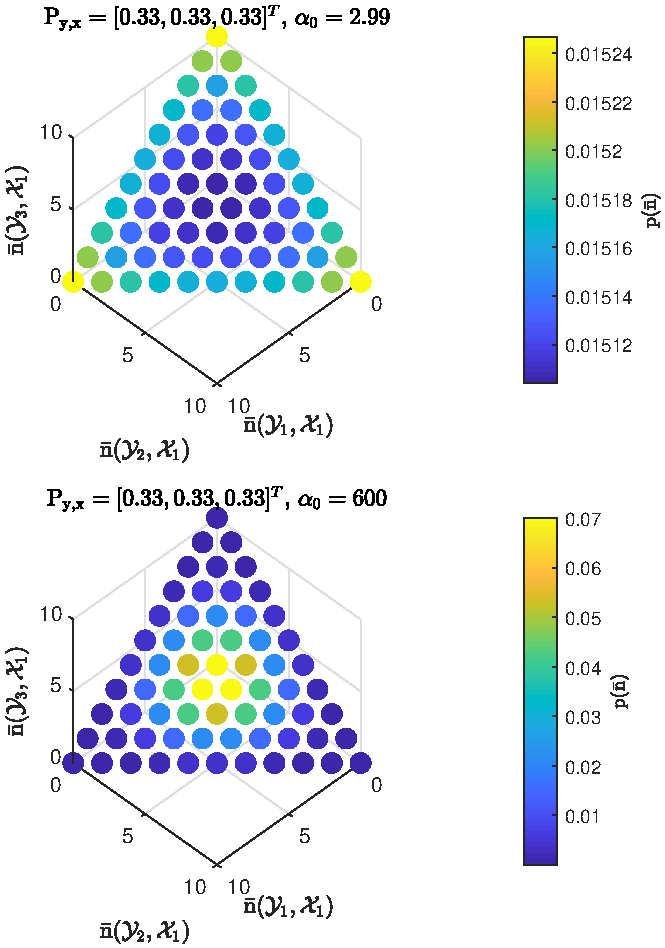
\includegraphics[scale=1.0]{P_nbar_a0.pdf}
\caption{$\Prm(\nbarrm)$ for different prior concentrations $\alpha_0$}
\label{fig:P_nbar_a0}
\end{figure}

\begin{figure}
\centering
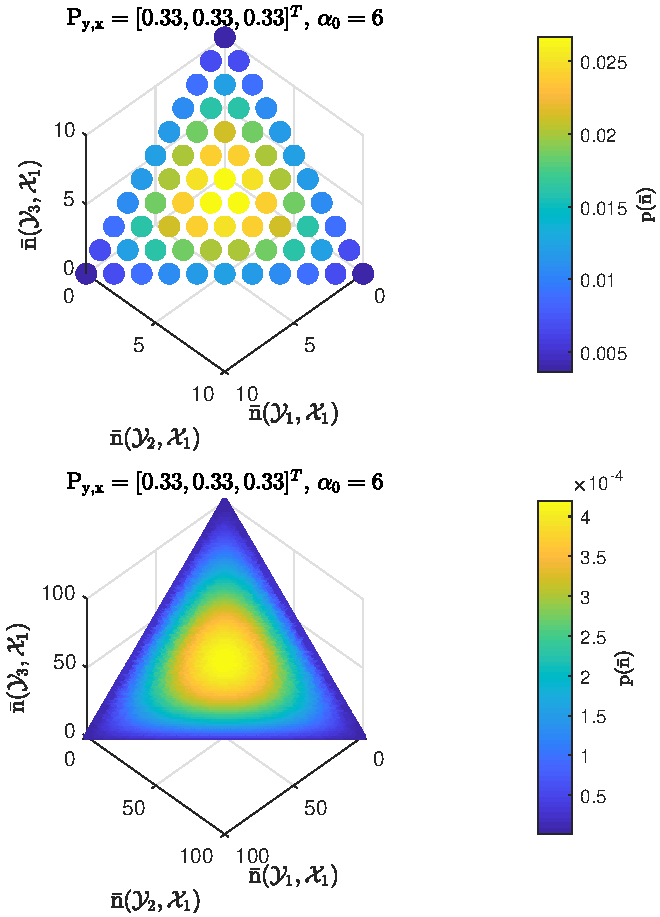
\includegraphics[scale=1.0]{P_nbar_N.pdf}
\caption{$\Prm(\nbarrm)$ for different training set sizes $N$}
\label{fig:P_nbar_N}
\end{figure}




\paragraph{Uniform Prior}

For the uniform distribution, $\alpha(y,x) = 1$,
\begin{IEEEeqnarray}{rCl} \label{P_D_io}
\Prm(\Drm) & = & \Mcal\big( \{N,|\Ycal||\Xcal|-1\} \big)^{-1} \Mcal\big( \bar{N}(\Drm) \big)^{-1} \;.
\end{IEEEeqnarray}
and
\begin{IEEEeqnarray}{rCl} \label{P_D_io}
\Prm(\nbarrm) & = & \Mcal\big( \{N,|\Ycal||\Xcal|-1\} \big)^{-1} \;.
\end{IEEEeqnarray}
The distribution of $\nbarrm$ is uniform over the set $\bar{\Ncal}$. As such, the PMF for $\Drm$ depends on the training data only through the multinomial coefficient. Consequently, the training sets are more probable when they are more ``concentrated''.





\subsubsection{Aggregation Properties}

As performed for the model $\theta$, a characterization of the function $\nbarrm$ integrated over the set $\Ycal$ will be found. Introduce the function $N' : \Dcal \to \Ncal'$, defined as
\begin{IEEEeqnarray}{rCl}
N'(x;D) & = & \sum_{y \in \Ycal} \bar{N}(y,x;D) = \sum_{n=1}^N \delta\big[ x,X_n \big]
\end{IEEEeqnarray}
where 
\begin{IEEEeqnarray}{rCl}
\Ncal' & = & \left\{ n' \in {\Zbb_{\geq 0}}^{\Xcal}: \sum_{x \in \Xcal} n'(x) = N \right\} \;.
\end{IEEEeqnarray}
Define the ``marginalized'' random function $\nrm'$ over the set $\Xcal$, defined as $\nrm'(x) \equiv \sum_{y \in \Ycal} \nbarrm(y,x) \equiv N'(\Drm)$. 


By the aggregation property of Multinomial random functions \cite{johnson}, the aggregation conditioned on the model $\theta$ is distributed as $\nrm' | \theta \sim \Mult(N,\theta')$. Similarly, by the aggregation property of Dirichlet-Multinomial functions \cite{johnson}, the new function without conditioning is distributed as $\nrm' \sim \DM(N,\alpha')$.

Also of interest is the distribution of $\nbarrm$ conditioned on its aggregation $\nrm'$. Using the multinomial distribution properties proven in Appendix \ref{app:mult}, it can be shown that when conditioned on the model $\theta$ as well, the PMF for $\nbarrm$ is
\begin{IEEEeqnarray}{rCl}
\Prm(\bar{\nrm} | \nrm' , \theta) & = & \prod_{x \in \Xcal} \Bigg[ \Mcal\big( \bar{\nrm}(\cdot,x) \big) \prod_{y \in \Ycal} \left(\frac{\theta(y,x)}{\theta'(x)}\right)^{\bar{\nrm}(y,x)} \Bigg] \\
& = & \prod_{x \in \Xcal} \Mult\Big( \bar{\nrm}(\cdot,x) ; \nrm'(x) , \theta(\cdot,x) / \theta'(x) \Big) \nonumber \;,
\end{IEEEeqnarray}
which has support $\bar{\nrm} \in \left\{ {\Zbb_{\geq 0}}^{\Ycal \times \Xcal} : \sum_{y \in \Ycal} \bar{n}(y,x) = \nrm'(x), \quad \forall x \in \Xcal \right\}$. Observe that conditioning on the aggregation renders the function segments $\nbarrm(\cdot,x)$ independent of one another and that they are also Multinomial, such that $\nbarrm(\cdot,x) | \nrm'(x),\theta \sim \Mult\big( \nrm'(x),\theta(\cdot,x) / \theta'(x) \big)$.

Similary, using the Dirichlet-Multinomial properties presented in Appendix \ref{app:DM_agg},
\begin{IEEEeqnarray}{rCl}
\Prm(\bar{\nrm} | \nrm') & = & \prod_{x \in \Xcal} \left[ \Mcal\big( \bar{\nrm}(\cdot,x) \big) \beta\big( \alpha(\cdot,x) \big)^{-1} \beta\big( \alpha(\cdot,x) + \bar{\nrm}(\cdot,x) \big) \right] \\
& = & \prod_{x \in \Xcal} \DM\Big( \bar{\nrm}(\cdot,x) ; \nrm'(x) , \alpha(\cdot,x) \Big) \nonumber \;,
\end{IEEEeqnarray}
with the same support as the model-conditioned case. Observe that conditioning on the aggregation renders the function segments $\nbarrm(\cdot,x)$ independent of one another and that they are also Dirichlet-Multinomial, such that $\nbarrm(\cdot,x) | \nrm'(x) \sim \DM\big( \nrm'(x),\alpha(\cdot,x) \big)$.












\subsection{Conditonal PMF $\Prm(\yrm | \xrm,\Drm)$}

As shown in Equation \eqref{eq:f_opt_xD}, the decision selected by the optimally designed function depends on $\Prm(\yrm | \xrm,\Drm)$, the distribution of the unobserved $\yrm$ conditioned on all observable random variables. This PMF will be expressed next.

First observe that since $\Prm(\Drm|\theta)$ is of exponential form, the Dirichlet prior $\prm(\theta)$ is its conjugate prior \cite{theodoridis-ML}; thus, the model posterior PDF given the training data is
\begin{IEEEeqnarray}{rCl}
\prm(\theta | \Drm) & = & \frac{\Prm(\Drm | \theta) \prm(\theta)}{\Prm(\Drm)} \\
& = & \beta \left( \alpha + \bar{N}(\Drm) \right)^{-1} \prod_{y \in \Ycal} \prod_{x \in \Xcal} 
\theta(y,x)^{\alpha(y,x) + \bar{N}(y,x;\Drm) - 1} \nonumber \;, 
\end{IEEEeqnarray}
a Dirichlet distribution with parameter function $\alpha + \bar{N}(\Drm)$.

This posterior distribution is of specific interest in the machine learning literature. While Bayesian techniques are used here, often point estimates of the model $\theta$ are formed; perhaps the most common approach is to form the Maximum a posteriori estimate,
\begin{IEEEeqnarray}{rCl}
\theta_\mathrm{MAP}(\Drm) & = & \argmax_{\theta \in \Theta} \Prm(\theta|\Drm) = \frac{\bar{N}(\Drm) + \alpha - 1}{N + \alpha_0 - |\Ycal||\Xcal|} \;.
\end{IEEEeqnarray}
This maximizing value is only valid when $\bar{N}(\Drm) >1$. For the uniform model prior, the maximizing value of the posterior is the empirical PMF $\bar{N}(\Drm) / N$.

Also, as the concentration parameter increases proportionately with increasing volumes of training data, as $N \to \infty$ the posterior converges to $\prm(\theta | \Drm) \to \delta\big( \theta - \bar{N}(\Drm) / N \big)$. Thus, as more data is collected, the model can be more positively identified and used to formulate minimum risk decisions. Conversely, as $\alpha_0 \to \infty$, the prior model certainty is stronger and the posterior trends toward $\prm(\theta | \Drm) \to \delta( \theta - \alpha / \alpha_0)$, independent of the training data.

Figure \ref{fig:P_theta_D} shows the influence of the training data on the model distribution; after conditioning on the training data (via $\nbarrm$), the PDF concentration shifts away from the models favored by the prior knowledge and towards other models that better account for the observations.

\begin{figure}
\centering
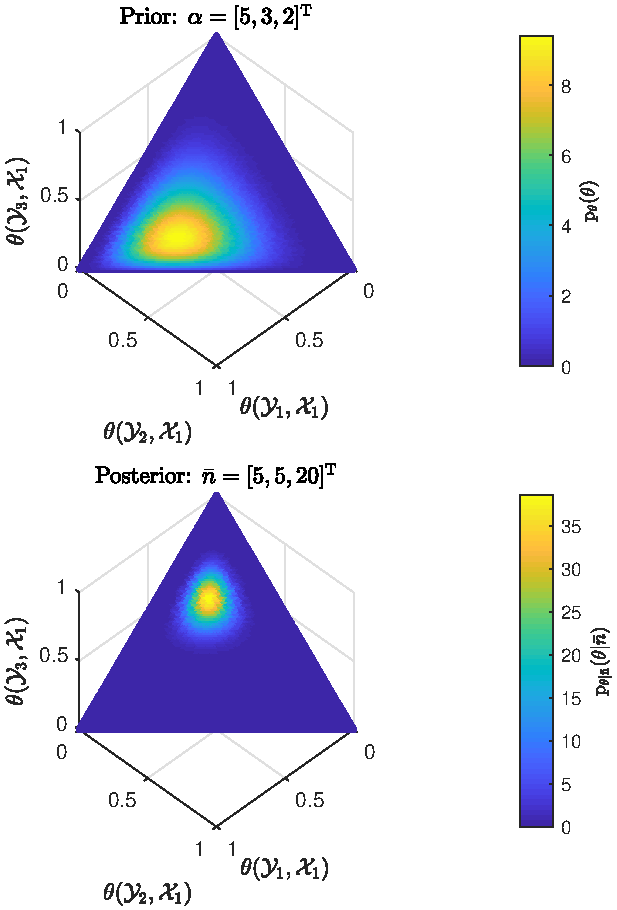
\includegraphics[scale=1.0]{P_theta_post.pdf}
\caption{Model $\theta$ PDF, prior and posterior}
\label{fig:P_theta_D}
\end{figure}





Next the joint PMF of $\yrm$ and $\xrm$ conditioned on the training data is expressed as
\begin{IEEEeqnarray}{rCl}
\Prm(\yrm,\xrm | \Drm) & = & \frac{\Erm_{\theta}\big[ \theta(\yrm,\xrm) \Prm(\Drm | \theta) \big]}{\Prm(\Drm)} = \mu_{\theta | \Drm}(\yrm,\xrm) \\
& = & \frac{\alpha(\yrm,\xrm) + \bar{N}(\yrm,\xrm;\Drm)}{\alpha_0 + N} \nonumber \\
& = & \left(\frac{\alpha_0}{\alpha_0 + N}\right) \frac{\alpha(\yrm,\xrm)}{\alpha_0} + \left(\frac{N}{\alpha_0 + N}\right) \frac{\bar{N}(\yrm,\xrm;\Drm)}{N} \nonumber \\
& = & \left(\frac{\alpha_0}{\alpha_0 + N}\right) \Prm(\yrm,\xrm) + \left(\frac{N}{\alpha_0 + N}\right) \frac{\bar{N}(\yrm,\xrm;\Drm)}{N} \nonumber \;.
\end{IEEEeqnarray}
This is a mixture distribution between the prior expectation $\Erm[\theta] = \alpha/\alpha_0$ and the empirical distribution $\bar{N}(\Drm)/N$. The more subjective the model prior (i.e. larger $\alpha_0$), the more the prior mean is favored; the more data, the more the empirical PMF is favored.

It is informative to compare the PMF $\Prm(\yrm,\xrm | \theta)$ with its ``estimate'' $\Prm(\yrm,\xrm | \Drm)$ and investigate the fit provided by different model priors. Consider a fixed model $\theta$ and user-selected prior PDF parameters $\alpha$. The expected value of the data-conditioned PMF is
\begin{IEEEeqnarray}{rCl}
\Erm_{\Drm|\theta}\big[ \Prm_{\yrm,\xrm}(y,x | \Drm) \big] & = & \frac{\alpha(y,x) + \Erm_{\bar{\nrm} | \theta}\big[ \bar{\nrm}(y,x) \big]}{\alpha_0+N} \\
& = & \left(\frac{\alpha_0}{\alpha_0 + N}\right) \frac{\alpha(y,x)}{\alpha_0} + \left(\frac{N}{\alpha_0 + N}\right) \theta(y,x) \nonumber \;,
\end{IEEEeqnarray}
a mixture of the prior expectation $\Erm[\theta] = \alpha/\alpha_0$ and the model $\theta$ itself; observe how as the volume of training data increases relative to the model prior concentration, the expectation trends away from the prior estimate and toward the true model. The expected bias of the model estimate $\Prm(\yrm,\xrm | \Drm)$ is
\begin{IEEEeqnarray}{rCl}
\mathrm{Bias}(y,x ; \alpha,\theta) & = & \Erm_{\Drm | \theta} \big[ \Prm_{\yrm,\xrm}(y,x | \Drm) - \theta(y,x) \big] \\
& = & \frac{\alpha_0}{\alpha_0+N} \left( \frac{\alpha(y,x)}{\alpha_0} - \theta(y,x) \right) \nonumber \;,
\end{IEEEeqnarray}
proportionate to the difference between $\theta$ and the data-independent expectation $\Erm[\theta]$. The scaling factor depends on the prior concentration and the number of training samples. For a highly subjective prior ($\alpha_0/N \to \infty$), the estimate becomes nearly independent of $\Drm$ and the scaling factor is unity. For an ``uncertain'' prior with low $\alpha_0$, the empirical distribution is used to estimate $\theta$ and the expected bias trends to zero.

The conditional variance of the estimate $\Prm(\yrm,\xrm | \Drm)$ is
\begin{IEEEeqnarray}{L}
\Crm_{\nbarrm | \theta} \big[\Prm_{\yrm,\xrm | \nbarrm}(\cdot,\cdot | \nbarrm) \big](y,x,y',x') \\
\quad = (\alpha_0+N)^{-2} \Sigma_{\nbarrm | \theta}(y,x,y',x') \nonumber \\
\quad = \frac{N}{(\alpha_0+N)^2} \big( \theta(y,x) \delta[y,y'] \delta[x,x'] - \theta(y,x) \theta(y',x') \big) \nonumber \;,
\end{IEEEeqnarray}
proportionate to the conditional variance of $\nbarrm$ given $\theta$. The scaling factor trends to zero with both increasing $\alpha_0$ and $N$.

Finally, consider the expected squared difference between the estimate and the true model,
\begin{IEEEeqnarray}{L}
\mathcal{E}(y,x,y',x;\alpha,\theta) \\
\quad = \Erm_{\nbarrm | \theta} \Big[ \big( \Prm_{\yrm,\xrm|\nbarrm}(y,x|\nbarrm) - \theta(y,x) \big) \big( \Prm_{\yrm,\xrm|\nbarrm}(y',x'|\nbarrm) - \theta(y',x') \big) \Big] \nonumber \\
\quad = \mathrm{Bias}(y,x;\alpha,\theta) \mathrm{Bias}(y',x';\alpha,\theta) + \Crm_{\nbarrm | \theta} \big[\Prm_{\yrm,\xrm | \nbarrm}(\cdot,\cdot | \nbarrm) \big](y,x,y',x') \nonumber \;,
\end{IEEEeqnarray}
which combines both the bias of the model estimate $\Prm(\yrm,\xrm | \Drm)$ and its variance. As $N \to \infty$, this function trends to zero and thus the underlying model $\theta$ is determined precisely. A more realistic and interesting case is estimation with a finite volume of training data. Specification of the Dirichlet model prior can be interpreted as providing a hypothesized distribution $\alpha/\alpha_0$ and a confidence level $\alpha_0$. Higher confidence reduces error due to the variance of the estimator, but increases the error due to bias between $\alpha/\alpha_0$ and $\theta$. Low confidence renders the estimate unbiased, but maximizes the estimator variance.

To exemplify how the model estimate $\Prm(\yrm,\xrm | \Drm)$ approximates $\theta$, consider the model and prior PMF shown in Figure \ref{fig:P_yx_error_N_0}. Note the significant mismatch. Figures \ref{fig:P_yx_error_a0_0_1} and \ref{fig:P_yx_error_a0_10} show how the expected value and variance of the estimate (represented by the blue markers and error bars, respectively) change for different values of $N$ and $\alpha_0$ . Each individual plot heading provides the error $\sqrt{\sum_{y \in \Ycal} \sum_{x \in \Xcal} \mathcal{E}(y,x,y,x;\alpha,\theta)}$ to assess the quality of the PMF estimate. Observe that for $N=1$, the high variance of the $\alpha_0 = 0.1$ estimate (favoring the empirical PMF) renders it worse than the $\alpha_0 = 10$ estimate; in fact, the variance is so high that the error exceeds that of the data-independent estimate $\alpha / \alpha_0$ (Figure \ref{fig:P_yx_error_N_0}). Conversely, for $N=10$, the confidence of the $\alpha_0 = 10$ estimate leads to high bias and the $\alpha_0 = 0.1$ estimate is superior.


\begin{figure}
\centering
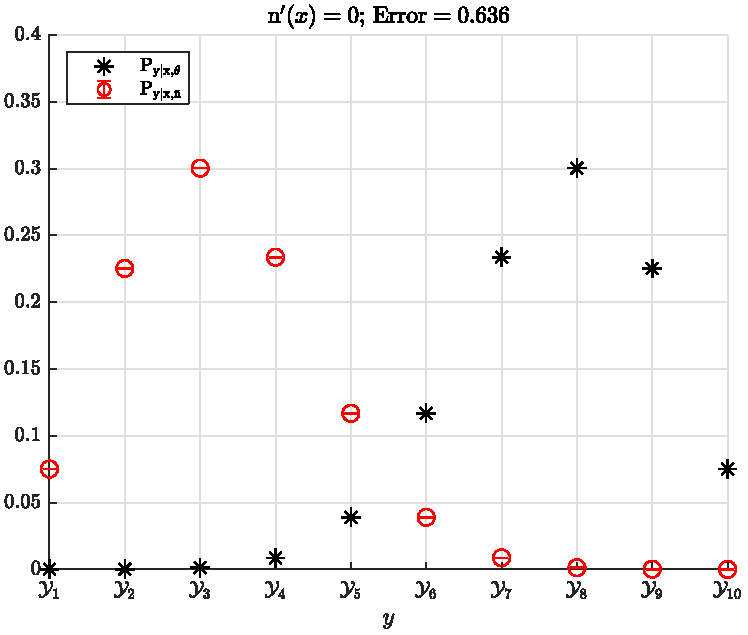
\includegraphics[scale=1.0]{P_yx_error_N_0.pdf}
\caption{Model $\theta$ estimate, no training data}
\label{fig:P_yx_error_N_0}
\end{figure}

\begin{figure}
\centering
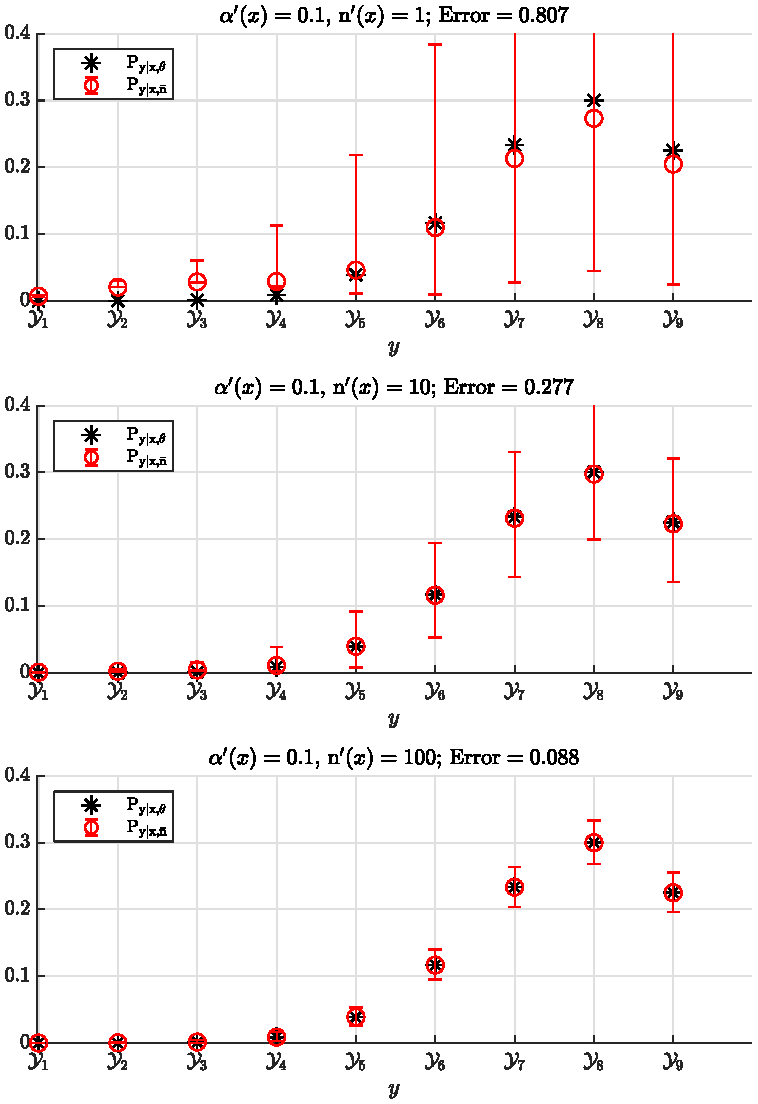
\includegraphics[scale=0.8]{P_yx_error_a0_0_1.pdf}
\caption{Model $\theta$ estimates, $\alpha_0 = 0.1$}
\label{fig:P_yx_error_a0_0_1}
\end{figure}

\begin{figure}
\centering
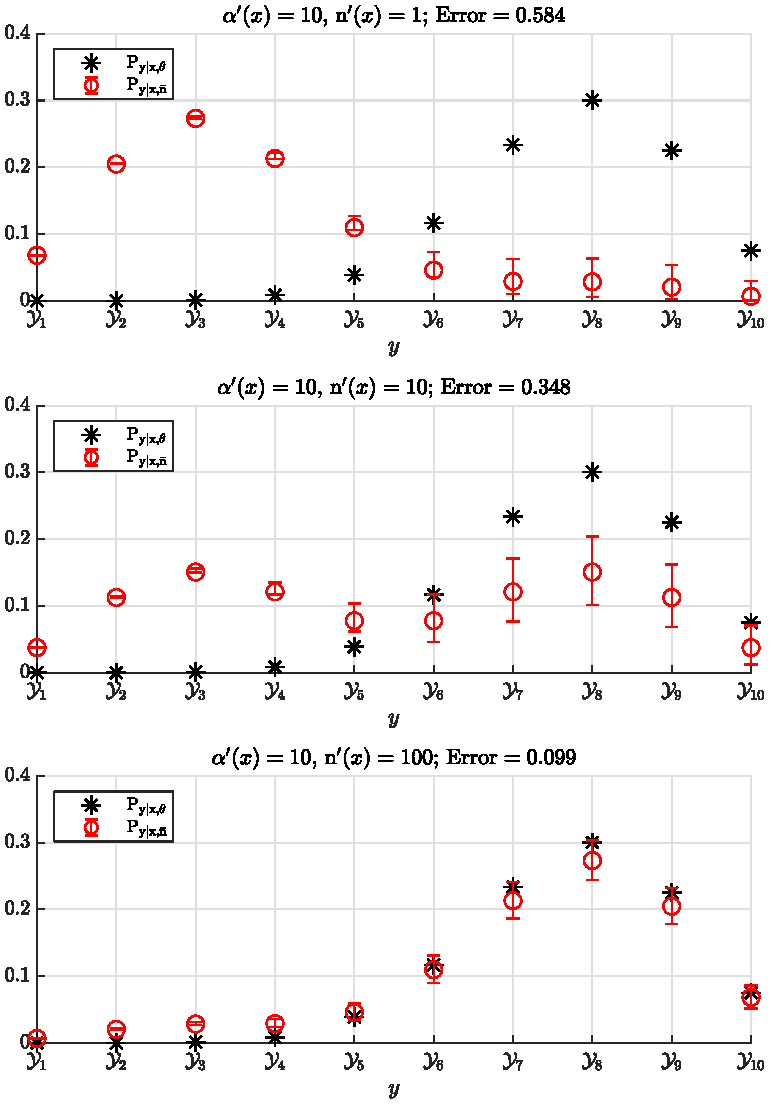
\includegraphics[scale=0.8]{P_yx_error_a0_10.pdf}
\caption{Model $\theta$ estimates, $\alpha_0 = 10$}
\label{fig:P_yx_error_a0_10}
\end{figure}


Proceeding towards an expression for the conditional estimate $\Prm(\yrm | \xrm,\Drm)$, the marginal distribution for $\xrm$ given $\Drm$ is
\begin{IEEEeqnarray}{rCl}
\Prm(\xrm | \Drm) & = & \frac{\alpha'(\xrm) + N'(\xrm;\Drm)}{\alpha_0 + N} \\
& = & \left(\frac{\alpha_0}{\alpha_0 + N}\right) \frac{\alpha'(\xrm)}{\alpha_0} + \left(\frac{N}{\alpha_0 + N}\right) \frac{N'(\xrm;\Drm)}{N} \nonumber \\
& = & \left(\frac{\alpha_0}{\alpha_0 + N}\right) \Prm(\xrm) + \left(\frac{N}{\alpha_0 + N}\right) \frac{N'(\xrm;\Drm)}{N} \nonumber \;.
\end{IEEEeqnarray}
Finally, the distribution of interest is generated via Bayes rule as
\begin{IEEEeqnarray}{rCl}
\Prm(\yrm | \xrm,\Drm) & = & \frac{\Prm(\yrm,\xrm | \Drm)}{\Prm(\xrm | \Drm)} = \frac{\alpha(\yrm,\xrm) + \bar{N}(\yrm,\xrm;\Drm)}{\alpha'(\xrm) + N'(\xrm;\Drm)} \\
& = & \left(\frac{\alpha'(\xrm)}{\alpha'(\xrm) + N'(\xrm;\Drm)}\right) \frac{\alpha(\yrm,\xrm)}{\alpha'(\xrm)} + \left(\frac{N'(\xrm;\Drm)}{\alpha'(\xrm) + N'(\xrm;\Drm)}\right) \frac{\bar{N}(\yrm,\xrm;\Drm)}{N'(\xrm;\Drm)} \nonumber \\
& = & \left(\frac{\alpha'(\xrm)}{\alpha'(\xrm) + N'(\xrm;\Drm)}\right) \Prm(\yrm | \xrm) + \left(\frac{N'(\xrm;\Drm)}{\alpha'(\xrm) + N'(\xrm;\Drm)}\right) \frac{\bar{N}(\yrm,\xrm;\Drm)}{N'(\xrm;\Drm)} \nonumber \;,
\end{IEEEeqnarray}

The last representation views the distribution as a convex combination of two conditional distributions. The first distribution $\Prm(\yrm | \xrm) = \alpha(\yrm,\xrm) / \alpha'(\xrm)$ is independent of the training data and based on the prior knowledge implied via the model PDF parameter; the second distribution is a ``conditional'' empirical PMF and depends on $\Drm$, not on $\alpha$. For both, only those values $\alpha$ and $\Drm$ corresponding to the observed value $\xrm$ shape the distribution. 

Similarly, the weighting factors are only influenced by these values. For $N'(\xrm;\Drm) = 0$ or as $\alpha_0 \to \infty$, the PMF trends toward the conditional distribution $\Prm(\yrm|\xrm)$, which only depends on the model parameter $\alpha$. As the number of training examples increases or as $\alpha_0 \to 0$, $\Prm(\yrm | \xrm,\Drm)$ trends towards the empirical conditional distribution. Note that for a given model $\theta$, the expected value of the conditional empirical distribution is 
\begin{IEEEeqnarray}{rCl}
\Erm_{\Drm | \theta}\left[ \frac{\bar{N}(\yrm,\xrm;\Drm)}{N'(\xrm;\Drm)} \right] & = & \Erm_{\bar{\nrm} | \theta}\left[ \frac{\bar{\nrm}(\yrm,\xrm)}{\nrm'(\xrm)} \right] = \Erm_{\nrm' | \theta}\left[ \frac{\Erm_{\bar{\nrm} | \nrm',\theta}\big[ \bar{\nrm}(\yrm,\xrm) \big]}{\nrm'(\xrm)} \right] \\
& = & \frac{\theta(\yrm,\xrm)}{\theta'(\xrm)} = \Prm(\yrm | \xrm,\theta) \nonumber \;,
\end{IEEEeqnarray}
where the properties of a multinomial distribution conditioned on its aggregation have been used. 

PGR: expectation given theta stuff??



\subsubsection{Representation using the complete model posterior}

Athough the distribution of interest has already been expressed in closed form, it is informative to introduce a different representation for the conditional PMF,
\begin{IEEEeqnarray}{rCl}
\Prm(\yrm | \xrm,\Drm) & = & \Erm_{\theta | \xrm,\Drm} \big[ \Prm(\yrm | \xrm,\theta) \big] \\
& = & \Erm_{\theta | \xrm,\Drm} \left[ \frac{\theta(\yrm,\xrm)}{\theta'(\xrm)} \right] \nonumber \;,
\end{IEEEeqnarray}
Just as $\Prm(\yrm,\xrm | \Drm)$ is an expectation of the model $\theta$ posterior conditioned on $\Drm$, $\Prm(\yrm | \xrm,\Drm)$ is an expectation of $\theta$ conditioned on both observed random variables. The expectation operates on the random function $\theta(\cdot,\xrm)$ normalized by its sum $\theta'(\xrm)$. 

The complete model posterior PDF is represented as
\begin{IEEEeqnarray}{rCl}
\prm(\theta | \xrm, \Drm) & = & \frac{\Prm(\xrm | \theta) \prm(\theta | \Drm)}{\Prm(\xrm | \Drm)} = \Erm_{\yrm | \xrm,\Drm} \big[ \prm(\theta | \yrm,\xrm,\Drm) \big] \\
& = & \sum_{y \in \Ycal} \frac{\alpha(y,\xrm) + \bar{N}(y,\xrm;\Drm)}{\alpha'(\xrm) + N'(\xrm;\Drm)} \Dir\bigg( \theta ; \alpha + \bar{N}\Big( \big( (y,\xrm),\Drm \big) \Big) \bigg) \nonumber \;,
\end{IEEEeqnarray}
where $\bar{N}\Big( \big( (y,x),D \big) \Big) = \bar{N}(D) + \delta[\cdot,y] \delta[\cdot,x]$. This is a mixture distribution whose weighting factors are, interestingly, the values of $\Prm(\yrm | \xrm,\Drm)$ itself. The PDF's being combined are Dirichlet distributions with different parameterizing functions $\alpha + \bar{N}\Big( \big( (y',\xrm),\Drm \big) \Big)$; additional emphasis is put on the $|\Ycal|$ different possible pairs $(y,x)$ including the observed value $\xrm$.

This posterior PDF shares the same asymptotic distributions with $\prm(\theta|\Drm)$. As $\alpha_0 \to \infty$ or $N \to \infty$, the $|\Ycal|$ Dirichlet mixture PDF's converge to the same impulsive distribution and thus $\prm(\theta|\xrm,\Drm)$ again trends toward $\delta(\theta - \alpha / \alpha_0)$ and $\delta\big( \theta - \bar{N}(\Drm)/N \big)$, respectively.

To confirm that the expectation produces the same distribution $\Prm(\yrm | \xrm,\Drm)$ displayed previously, use the properties of a Dirichlet random function conditioned on its aggregation to show that $\Erm_{\theta}\big[ \theta(y,x) / \theta'(x) \big] = \alpha(y,x) / \alpha'(x)$. Thus, the PMF is evaulated as
\begin{IEEEeqnarray}{rCl}
\Prm(\yrm | \xrm,\Drm) & = & \sum_{y' \in \Ycal} \frac{\alpha(y',\xrm) + \bar{N}(y',\xrm;\Drm)}{\alpha'(\xrm) + N'(\xrm;\Drm)} \\
&& \qquad \left( \frac{\alpha(\yrm,\xrm) + \bar{N}(\yrm,\xrm;\Drm) + \delta[y',\yrm] \delta[\xrm,\xrm]}{\alpha'(\xrm) + N'(\xrm;\Drm) + \delta[\xrm,\xrm]} \right) \nonumber \\
& = & \frac{\alpha(\yrm,\xrm) + \bar{N}(\yrm,\xrm;\Drm)}{\alpha'(\xrm) + N'(\xrm;\Drm)} \nonumber \;.
\end{IEEEeqnarray}







\paragraph{Uniform Prior}

For the uniform model prior PDF, the conditional distribution is
\begin{IEEEeqnarray}{rCl} \label{P_y_xD_uniform}
\Prm(\yrm | \xrm,\Drm) & = & \frac{\bar{N}(\yrm,\xrm;\Drm)+1}{N'(\xrm;\Drm) + |\Ycal|} \\
& = & \left( \frac{|\Ycal|}{N'(\xrm;\Drm) + |\Ycal|} \right) \frac{1}{|\Ycal|} + \nonumber \\
&& \quad \left( \frac{N'(\xrm;\Drm)}{N'(\xrm;\Drm) + |\Ycal|} \right) \frac{\bar{N}(\yrm,\xrm;\Drm)}{N'(\xrm;\Drm)} \nonumber \;.
\end{IEEEeqnarray}
Now the prior PMF contribution $\Prm(\yrm|\xrm)$ is a uniform distribution over the $|\Ycal|$ possible outputs. The weighting factors are controlled by $\alpha'(\xrm) = |\Ycal|$; the more possible outcomes $|\Ycal|$ there are for a given training set size, the more the conditional distribution trends toward the uniform PMF implied by the model prior.



















\newpage



\section{Applications to Common Loss Functions MAIN}

PGR: equations, plots for specific theta results? subjective/objective tradeoff??? alpha/theta mismatch results???

In this section, loss functions typical for classification and regression applications, specifically the 0-1 loss function and the squared-error loss function, are adopted. Optimal learners $f^*(\xrm;\Drm)$ are found and the corresponding minimum risk $\Rcal(f^*)$ is assessed.

As shown in Equation \eqref{eq:f_opt_xD}, the decision expressed for a given input $\xrm$ and training set $\Drm$ minimizes the metric
\begin{IEEEeqnarray}{L} \label{eq:E_y|xD L}
\Erm_{\yrm | \xrm,\Drm} \big[ \mathcal{L}(h,\yrm) \big] = \sum_{y \in \Ycal} \mathcal{L}(h,y) \Prm_{\yrm | \xrm,\Drm}(y | \xrm,\Drm) \\
= \frac{\sum_{y \in \Ycal} \alpha(y,\xrm) \mathcal{L}(h,y) + \sum_{y \in \Ycal} \bar{N}(y,\xrm;\Drm) \mathcal{L}(h,y)}{\alpha'(\xrm) + N'(\xrm;\Drm)} \nonumber \\
= \left(\frac{\alpha'(\xrm)}{\alpha'(\xrm) + N'(\xrm;\Drm)}\right) \sum_{y \in \Ycal} \frac{\alpha(y,\xrm)}{\alpha'(\xrm)} \mathcal{L}(h,y) + \left(\frac{N'(\xrm;\Drm)}{\alpha'(\xrm) + N'(\xrm;\Drm)}\right) \sum_{y \in \Ycal} \frac{\bar{N}(y,\xrm;\Drm)}{N} \mathcal{L}(h,y) \nonumber \\
= \left(\frac{\alpha'(\xrm)}{\alpha'(\xrm) + N'(\xrm;\Drm)}\right) \Erm_{\yrm | \xrm}\big[ \mathcal{L}(h,\yrm) \big] + \left(\frac{N'(\xrm;\Drm)}{\alpha'(\xrm) + N'(\xrm;\Drm)}\right) \frac{\sum_{n=1}^N \delta\big[ \xrm,\Xrm_n \big] \mathcal{L}\big( h,\Yrm_n \big)}{\sum_{n=1}^N \delta\big[ \xrm,\Xrm_n \big]} \nonumber \;.
\end{IEEEeqnarray}

The expectation can be represented as a convex combination of two expected losses. The first expected loss is evaluated with respect to the conditional distribution $\Prm(\yrm|\xrm) = \alpha(\yrm,\xrm) / \alpha'(\xrm)$, which reflects the prior knowledge imparted by the model parameter $\alpha$. The second term is a conditional emprical loss, or the average loss among samples $\Yrm_n$ whose corresponding values $\Xrm_n$ match the observed value $\xrm$. The convex weights are inherited from the conditional distribution $\Prm(\yrm|\xrm,\Drm)$; thus, for a given observation $\xrm$, the model prior parameter $\alpha'(\xrm)$ and the number of matching training samples $N'(\xrm;\Drm)$ dictate which of the two expectations are emphasized.




\subsection{The Squared-Error Loss}

PGR: Use finite hypothesis space instead, wait for continuous DP???

The squared-error (SE) loss function is arguably the most commonly used loss function for regression, or in fact for any estimation problem. This can be attributed to its quadratic form, which enables a closed-form expression of the minimizing estimation function $f^*(\Drm)$.

It is assumed that both the unobserved random variable $\yrm$ and the observed $\xrm$ are scalar and have real numerical values; that is, $\Ycal \subset \Rbb$ and $\Xcal \subset \Rbb$. Additionally, the learning function's estimate is a real number; thus, $\Hcal = \Rbb \supset \Ycal$.

The loss function is defined as
\begin{equation}
\mathcal{L}(h,y) = (h-y)^2 \;.
\end{equation}
Substituting into \eqref{eq:risk_cond}, the conditional risk for a given estimator is 
\begin{IEEEeqnarray}{rCl}
\Rcal_{\Theta}(f;\theta) & = & \Erm_{\Drm | \theta} \bigg[ \Erm_{\yrm,\xrm | \theta} \Big[ \big( f(\xrm;\Drm)-\yrm \big)^2 \Big] \bigg] \\
& = & \Erm_{\xrm | \theta} \Big[ \Erm_{\yrm | \xrm,\theta} \big[ (\yrm - \mu_{\yrm | \xrm,\theta})^2 \big] \Big] + \Erm_{\xrm,\Drm | \theta} \Big[ \big( f(\xrm;\Drm) - \mu_{\yrm | \xrm,\theta} \big)^2 \Big] \nonumber \\
& = & \Erm_{\xrm | \theta} \left[ \Sigma_{\yrm | \xrm,\theta} \right] + \Erm_{\xrm,\Drm | \theta} \Big[ \big( f(\xrm;\Drm) - \mu_{\yrm | \xrm,\theta} \big)^2 \Big] \nonumber \;,
\end{IEEEeqnarray}
a sum of two terms. The first term is independent of the estimator; this irreducible risk is the expected conditional variance when the model $\theta$ is known. The second term is the additional risk due to the model uncertainty; it is the expected squared-error between the estimator output and the clairvoyant estimate $\mu_{\yrm | \xrm,\theta}$.

Performing the expectation with respect to the Dirichlet model prior, the Bayes risk is 
\begin{IEEEeqnarray}{rCl} \label{eq:risk_SE}
\Rcal(f) & = & \Erm_{\theta} \Bigg[ \Erm_{\Drm | \theta} \bigg[ \Erm_{\yrm,\xrm | \theta} \Big[ \big( f(\xrm;\Drm)-\yrm \big)^2 \Big] \bigg] \Bigg] \\
& = & \Erm_{\xrm,\Drm} \bigg[ \Erm_{\yrm | \xrm,\Drm} \Big[ \big( f(\xrm;\Drm)-\yrm \big)^2 \Big] \bigg] \nonumber \;.
\end{IEEEeqnarray}





\subsubsection{Optimal Estimate: the Posterior Mean}

PGR: plots?

To find the optimal estimator, the squared-error loss is substituted into \eqref{eq:f_opt_xD}; note that the objective function is quadratic over the argument $h$. It is easily shown that the second derivative with respect to $h$ is positive and thus the function is convex; as such, the minimizing decision $h$ is the sole stationary point. Setting the first derivative of the function to zero, the optimal estimate is the expected value of $\yrm$ given the training data and the observed value $\xrm$, such that
\begin{IEEEeqnarray}{rCl} \label{eq:f_opt_SE}
f^*(\xrm;\Drm) & = & \argmin_{h \in \Rbb} \Erm_{\yrm | \xrm,\Drm} \left[ (h-\yrm)^2 \right] = \mu_{\yrm | \xrm,\Drm} \\
& = & \left( \frac{\alpha'(\xrm)}{\alpha'(\xrm) + N'(\xrm;\Drm)} \right) \sum_{y \in \Ycal} y \frac{\alpha(y,\xrm)}{\alpha'(\xrm)} \nonumber \\
&& \quad + \left( \frac{N'(\xrm;\Drm)}{\alpha'(\xrm) + N'(\xrm;\Drm)} \right) \sum_{y \in \Ycal} y \frac{\bar{N}(y,\xrm;\Drm)}{N'(\xrm;\Drm)} \nonumber \\
& = & \left( \frac{\alpha'(\xrm)}{\alpha'(\xrm) + N'(\xrm;\Drm)} \right) \mu_{\yrm | \xrm} \nonumber \\
&& \quad + \left( \frac{N'(\xrm;\Drm)}{\alpha'(\xrm) + N'(\xrm;\Drm)} \right) \frac{\sum_{n=1}^N \delta\big[ \xrm,\Xrm_n \big] \Yrm_n}{N'(\xrm;\Drm)} \nonumber \;.
\end{IEEEeqnarray}

The optimal estimate is interpreted as a convex combination of two separate estimates - the expected value of $\yrm$ conditioned on the observed $\xrm$ and the mean of the training values $\Yrm_n$ which have a value $\Xrm_n$ matching the observed value $\xrm$. The weighting factors are the same as those of $\Prm(\yrm | \xrm,\Drm)$; thus, stronger prior information (larger $\alpha'(\xrm)$) provides more weight to the estimate $\mu_{\yrm|\xrm}$ and more voluminous training data puts emphasis on the empirical conditional mean.

Another interesting form for the optimal estimator is $f^*(\xrm;\Drm) = \Erm_{\theta | \xrm,\Drm} \left[ \mu_{\yrm | \xrm,\theta} \right]$. If the model $\theta$ were known, then the expectation $\mu_{\yrm | \xrm,\theta}$ would be optimal; instead, all such estimates are weighted and combined via the expectation over the model posterior PDF $\Prm(\theta | \xrm,\Drm)$.


\subparagraph{Uniform Prior}

The optimal estimator for a uniform prior is
\begin{IEEEeqnarray}{rCl}
f^*(\xrm;\Drm) & = & \mu_{\yrm | \xrm,\Drm}(\xrm, \Drm) \\
& = & \left( \frac{|\Ycal|}{N'(\xrm;\Drm) + |\Ycal|} \right) \frac{1}{|\Ycal|} \sum_{y \in \Ycal} y + \nonumber \\
&& \quad \left( \frac{N'(\xrm;\Drm)}{N'(\xrm;\Drm) + |\Ycal|} \right) \sum_{y \in \Ycal} y \frac{\bar{N}(y,\xrm;D)}{N'(\xrm;\Drm)} \nonumber \\
& = & \left( \frac{|\Ycal|}{N'(\xrm;\Drm) + |\Ycal|} \right) \frac{1}{|\Ycal|} \sum_{y \in \Ycal} y + \nonumber \\
&& \quad \left( \frac{N'(\xrm;\Drm)}{N'(\xrm;\Drm) + |\Ycal|} \right) \frac{\sum_{n=1}^N \delta\big[ \xrm,\Xrm_n \big] \Yrm_n}{N'(\xrm;\Drm)} \nonumber \;.
\end{IEEEeqnarray}

Now, the model prior contribution to the weighting factors depends on the cardinality $|\Ycal|$ and the prior expectation is simply the average of the elements of $\Ycal$.




\subsubsection{Minimum Risk: the Expected Posterior Variance}

Substituting the optimal estimator \eqref{eq:f_opt_SE} into Equation \eqref{eq:risk_SE}, the minimum Bayes risk is the expected conditional variance
\begin{IEEEeqnarray}{rCl}
\Rcal(f^*) & = & \Erm_{\xrm,\Drm} \left[ \Sigma_{\yrm | \xrm,\Drm} \right] \\
& = & \Erm_{\xrm,\theta} \left[ \Sigma_{\yrm | \xrm,\theta} \right] + \Erm_{\xrm,\Drm} \left[ \Crm_{\theta | \xrm,\Drm} \left[ \mu_{\yrm | \xrm,\theta} \right] \right] \nonumber \;.
\end{IEEEeqnarray}
The first term is the expected irreducible risk. The second term is the expected variance of the clairvoyant estimate $\mu_{\yrm | \xrm,\theta}$, where the variance is evaluated with respect to the model posterior PDF $\prm(\theta|\xrm,\Drm)$

Using the sufficient statistic for $\Drm$, the minimum risk can also be represented as $\Erm_{\xrm,\nbarrm} \left[ \Sigma_{\yrm | \xrm,\nbarrm} \right]$; as such, the expectations are performed over $\nbarrm$. Decompose the conditional variance as
\begin{IEEEeqnarray}{rCl}
\Sigma_{\yrm | \xrm,\nbarrm} & = & \Erm_{\yrm | \xrm,\nbarrm}[\yrm^2] - {\mu_{\yrm | \xrm,\nbarrm}}^2 
\end{IEEEeqnarray}
and assess the expected values of these terms separately. The first term is simply
\begin{IEEEeqnarray}{L}
\Erm_{\xrm,\nbarrm} \left[ \Erm_{\yrm | \xrm,\nbarrm}[\yrm^2] \right] \\
\quad = \Erm_{\yrm}[\yrm^2] = \sum_{y \in \Ycal} y^2 \left( \sum_{x \in \Xcal} \frac{\alpha(y,x)}{\alpha_0} \right) \nonumber \\
\quad = \Erm_{\xrm} \big[ \Erm_{\yrm | \xrm} [ \yrm^2 ] \big] = \sum_{x \in \Xcal} \frac{\alpha'(x)}{\alpha_0} \sum_{y \in \Ycal} y^2 \frac{\alpha(y,x)}{\alpha'(x)} \nonumber \;,
\end{IEEEeqnarray}
where the different functions of $\alpha$ are represented by the PMF's of $\yrm$ and $\xrm$. Next, find, 
\begin{IEEEeqnarray}{L}
\Erm_{\xrm,\nbarrm} \Big[ {\mu_{\yrm | \xrm,\nbarrm}}^2 \Big] =
\sum_{\bar{n} \in \bar{\Ncal}} \sum_{x \in \Xcal} \Prm_{\xrm,\nbarrm}(x,\bar{n}) \left( \sum_{y \in \Ycal} y \Prm_{\yrm | \xrm,\nbarrm}(y | x,\bar{n}) \right)^2 \\
= \sum_{x \in \Xcal} \sum_{y \in \Ycal} y \sum_{y' \in \Ycal} y' \Erm_{\nbarrm} \left[ \frac{\big( \alpha(y,x)+\bar{\nrm}(y,x) \big) \big(\alpha(y',x)+\bar{\nrm}(y',x) \big)}{(\alpha_0+N) \big(\alpha'(x) + \nrm'(x) \big)} \right] \nonumber \\
= \sum_{x \in \Xcal} \sum_{y \in \Ycal} y \sum_{y' \in \Ycal} y' \Erm_{\nrm'} \left[ \frac{\Erm_{\nbarrm | \nrm'} \left[ \big( \alpha(y,x)+\bar{\nrm}(y,x) \big) \big(\alpha(y',x)+\bar{\nrm}(y',x) \big) \right]}{(\alpha_0+N) \big(\alpha'(x) + \nrm'(x) \big)} \right] \nonumber \\
= \sum_{x \in \Xcal} \sum_{y \in \Ycal} y \sum_{y' \in \Ycal} y' \frac{\Erm_{\nrm'} \Big[ \nrm'(x) \alpha'(x) \alpha(y,x) \delta[y,y'] + \alpha'(x) \big( \alpha'(x) + \nrm'(x) + 1 \big) \alpha(y,x) \alpha(y',x) \Big]}{(\alpha_0+N) \big(\alpha'(x) + 1 \big) \alpha'(x)^2} \nonumber \\
= \sum_{x \in \Xcal} \frac{\Erm_{\nrm'} \Big[ \nrm'(x) \Erm_{\yrm|\xrm}[\yrm^2](x) + \alpha'(x) \big( \alpha'(x) + \nrm'(x) + 1 \big) \mu_{\yrm|\xrm}(x)^2 \Big]}{(\alpha_0+N) \big(\alpha'(x) + 1 \big)} \nonumber \\
= \sum_{x \in \Xcal} \frac{N \alpha'(x) \Erm_{\yrm|\xrm}[\yrm^2](x) + \alpha'(x) \big( \alpha_0 \alpha'(x) + N \alpha'(x) + 1 \big) \mu_{\yrm|\xrm}(x)^2 }{\alpha_0 (\alpha_0+N) \big(\alpha'(x) + 1 \big)} \nonumber \\
= \Erm_{\xrm} \left[ \frac{N \Erm_{\yrm|\xrm}[\yrm^2] + \big( \alpha_0 \alpha'(x) + N \alpha'(x) + \alpha_0 \big) {\mu_{\yrm|\xrm}}^2 }{(\alpha_0+N) \big( \alpha'(x)+1 \big)} \right] \nonumber \;.
\end{IEEEeqnarray}
%\begin{IEEEeqnarray}{L}
%\Erm_{\xrm,\nbarrm} \Big[ {\mu_{\yrm | \xrm,\nbarrm}}^2 \Big] =
%\sum_{\bar{n} \in \bar{\Ncal}} \sum_{x \in \Xcal} \Prm_{\xrm,\nbarrm}(x,\bar{n}) \left( \sum_{y \in \Ycal} y \Prm_{\yrm | \xrm,\nbarrm}(y | x,\bar{n}) \right)^2 \\
%= \sum_{x \in \Xcal} \sum_{y \in \Ycal} y \sum_{y' \in \Ycal} y' \Erm_{\nbarrm} \left[ \frac{\big( \alpha(y,x)+\bar{\nrm}(y,x) \big) \big(\alpha(y',x)+\bar{\nrm}(y',x) \big)}{(\alpha_0+N) \big(\alpha'(x) + \nrm'(x) \big)} \right] \nonumber \\
%= \sum_{x \in \Xcal} \sum_{y \in \Ycal} y \sum_{y' \in \Ycal} y' \Erm_{\nrm'} \left[ \frac{\Erm_{\nbarrm | \nrm'} \left[ \big( \alpha(y,x)+\bar{\nrm}(y,x) \big) \big(\alpha(y',x)+\bar{\nrm}(y',x) \big) \right]}{(\alpha_0+N) \big(\alpha'(x) + \nrm'(x) \big)} \right] \nonumber \\
%= \sum_{x \in \Xcal} \sum_{y \in \Ycal} y \sum_{y' \in \Ycal} y' \frac{\Erm_{\nrm'} \Big[ \nrm'(x) \frac{\alpha(y,x)}{\alpha'(x)} \delta[y,y'] + \alpha'(x) \big( \alpha'(x) + \nrm'(x) + 1 \big) \frac{\alpha(y,x)}{\alpha'(x)} \frac{\alpha(y',x)}{\alpha'(x)} \Big]}{(\alpha_0+N) \big(\alpha'(x) + 1 \big)} \nonumber \\
%= \sum_{x \in \Xcal} \sum_{y \in \Ycal} y \sum_{y' \in \Ycal} y' \left(\frac{\alpha'(x)}{\alpha_0}\right)  \frac{N \frac{\alpha(y,x)}{\alpha'(x)} \delta[y,y'] + \big( N \alpha'(x) + \alpha_0 \alpha'(x) + \alpha_0 \big) \frac{\alpha(y,x)}{\alpha'(x)} \frac{\alpha(y',x)}{\alpha'(x)}}{(\alpha_0+N) \big( \alpha'(x)+1 \big)} \nonumber \\
%= \sum_{x \in \Xcal} \left(\frac{\alpha'(x)}{\alpha_0}\right)  \frac{N \left( \sum_{y \in \Ycal} \frac{\alpha(y,x)}{\alpha'(x)} y^2 \right) + \big( N \alpha'(x) + \alpha_0 \alpha'(x) + \alpha_0 \big) \left( \sum_{y \in \Ycal} \frac{\alpha(y,x)}{\alpha'(x)} y \right)^2 }{(\alpha_0+N) \big( \alpha'(x)+1 \big)} \nonumber \;.
%\end{IEEEeqnarray}
The above formulation exploits the statistical characterization of the aggregation, $\nrm' \sim \DM(N,\alpha')$; also used is the property that the Dirichlet-Multinomial random function $\nbarrm$ conditioned on its aggregation $\nrm'$ yields independent  conditional DM functions $\bar{\nrm}(\cdot,x) | \nrm'(x) \sim \DM\big( \nrm'(x),\alpha(\cdot,x) \big)$.

PGR: move to appendix???

Finally, combine the two formulas to represent the mininum Bayes risk,
\begin{IEEEeqnarray}{L}
\Rcal(f^*) = \Erm_{\xrm,\nbarrm} \left[ \Erm_{\yrm | \xrm,\nbarrm}[\yrm^2] - {\mu_{\yrm | \xrm,\nbarrm}}^2 \right] \\
= \Erm_{\xrm} \left[ \frac{\alpha_0 \alpha'(\xrm) + N \alpha'(\xrm) + \alpha_0}{(\alpha_0+N) \big( \alpha'(\xrm)+1 \big)} \Sigma_{\yrm | \xrm} \right] \nonumber \\
= \Erm_{\xrm} \left[ \frac{\Prm(\xrm) + (\alpha_0+N)^{-1}}{\Prm(\xrm) + \alpha_0^{-1}} \Sigma_{\yrm | \xrm} \right] \nonumber \;.
\end{IEEEeqnarray}
The minimum risk is a convex combination of scaled conditional variances for the different PMF's $\Prm(\yrm | \xrm) = \alpha(\yrm,\xrm)/\alpha'(\xrm)$. The convex coefficients are values from the prior marginal distribution $\Prm(\xrm) = \alpha'(\xrm)/\alpha_0$. 

The scaling factor for each term $\Sigma_{\yrm | \xrm}$ depends on the marginal value $\Prm(\xrm)$, as well as on the prior concentration $\alpha_0$ and the number of training samples $N$. Observe that with no training data ($N = 0$), the scaling factor becomes unity and the risk is $\Rcal(f^*) = \Erm_{\xrm} \left[ \Sigma_{\yrm | \xrm} \right]$. Conversely, as $N \to \infty$, the Bayes risk is $\Rcal(f^*) = \Erm_{\xrm} \left[ \frac{\Prm(\xrm)}{\Prm(\xrm) + \alpha_0^{-1}} \Sigma_{\yrm | \xrm} \right]$; note that this minimal risk is also equivalent to $\Erm_{\xrm,\theta} \left[ \Sigma_{\yrm | \xrm,\theta} \right]$, the expected variance of the clairvoyant learner. Also, as the model concentration parameter $\alpha_0 \to 0$, the risk trends to zero (for $N > 0$); as $\alpha_0 \to \infty$, the risk trends toward $\Erm_{\xrm} \left[ \Sigma_{\yrm | \xrm} \right]$.

To illustrate these trends, explicitly define the sets $\Ycal = \{ i/M_{\yrm} : i = 0,\ldots,M_{\yrm}-1 \}$ and $\Xcal = \{ i/M_{\xrm} : i = 0,\ldots,M_{\xrm}-1 \}$. Assume that the conditional variance $\Sigma_{\yrm | \xrm}$ is independent of $\xrm$; in this case, the squared-error becomes the conditional variance scaled by a factor dependent on the marginal distribution $\Prm(\xrm)$, such that $\Rcal(f^*) = \Sigma_{\yrm | \xrm} \Erm_{\xrm} \left[ \frac{\Prm(\xrm) + (\alpha_0+N)^{-1}}{\Prm(\xrm) + \alpha_0^{-1}} \right]$.  Figures \ref{fig:Risk_SE_Dir_IO_N_leg_a0} and \ref{fig:Risk_SE_Dir_IO_a0_leg_N} display how the risk changes with $N$ and $\alpha_0$ for fixed $\Prm(\yrm|\xrm)$ and $\Prm(\xrm)$.

\begin{figure}
\centering
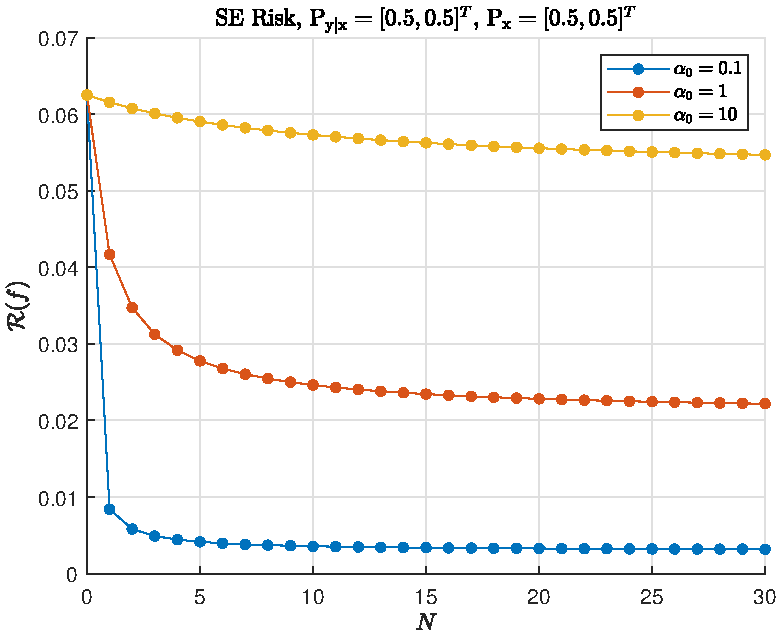
\includegraphics[scale=1.0]{Risk_SE_Dir_IO_N_leg_a0.pdf}
\caption{Optimal SE Risk for different training set sizes $N$}
\label{fig:Risk_SE_Dir_IO_N_leg_a0}
\end{figure}

\begin{figure}
\centering
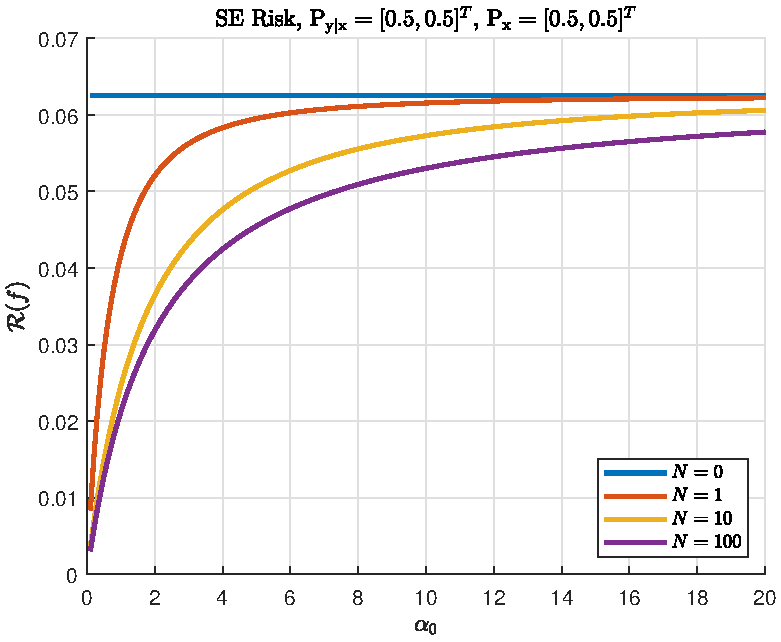
\includegraphics[scale=1.0]{Risk_SE_Dir_IO_a0_leg_N.pdf}
\caption{Optimal SE Risk for different prior concentrations $\alpha_0$}
\label{fig:Risk_SE_Dir_IO_a0_leg_N}
\end{figure}

It may not seem intutitve for the risk to decrease when $\alpha_0$ is smaller -- the variance of the model $\theta$ increases and the prior knowledge is less definitive. This is a result of the Dirichlet PDF weight shifting towards the $|\Ycal||\Xcal|$ models which have $\ell_0$ norms satisfying $\| \theta \|_0 = 1$. Although these PMF's are maximally separated (and uncorrelated), they all have zero variance and thus zero risk. The optimal learner will simply use the empirical distribution supplied via the training data - this allows exact identification of $\theta$ with a single training pair and leads to predictions that match the single element represented in $\Yrm$.

It is also informative to visualize how the minimum squared-error changes for fixed volume of training data $N$ and a fixed prior concentration $\alpha_0$. First, consider how the risk changes with the conditional PMF $\Prm(\yrm | \xrm)$. Figure \ref{fig:Risk_SE_Dir_IO_Pyx} demonstrates how the squared-error trends towards zero for PMFs that have $\ell_0$-norm equal to one.
\begin{figure}
\centering
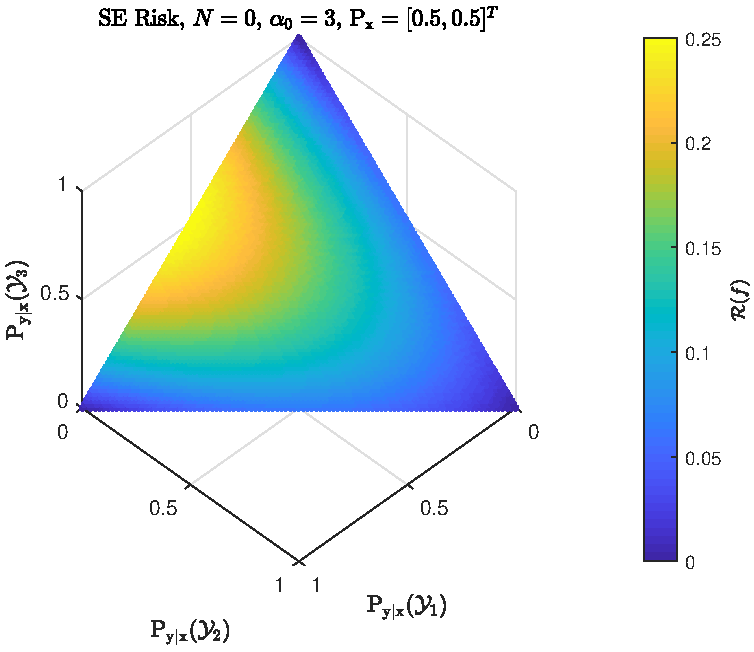
\includegraphics[scale=1.0]{Risk_SE_Dir_IO_Pyx.pdf}
\caption{Optimal SE Risk for different PMF's $\Prm(\yrm | \xrm)$}
\label{fig:Risk_SE_Dir_IO_Pyx}
\end{figure}
Next, consider the effect of the marginal distribution $\Prm(\xrm)$. Figure \ref{fig:Risk_SE_Dir_IO_Px_N_10_a0_1} demonstrates how the risk changes with this marginal PMF. Observe that the risk is maximal at the distributions satisfying $\| \Prm_{\xrm} \|_0 = 1$; the scaling factor for the conditional variance $\Sigma_{\yrm | \xrm}$ becomes $\frac{1 + (\alpha_0+N)^{-1}}{1 + \alpha_0^{-1}}$. Conversely, for $\Prm(\xrm) = 1/|\Xcal|$ the scaling factor becomes $\frac{|\Xcal|^{-1} + (\alpha_0+N)^{-1}}{|\Xcal|^{-1} + \alpha_0^{-1}}$ and the risk is minimal. Figures \ref{fig:Risk_SE_Dir_IO_N_leg_Px} and \ref{fig:Risk_SE_Dir_IO_a0_leg_Px} show how different marginals $\Prm(\xrm)$ affect the risk as a function of $N$ and $\alpha_0$, respectively.

\begin{figure}
\centering
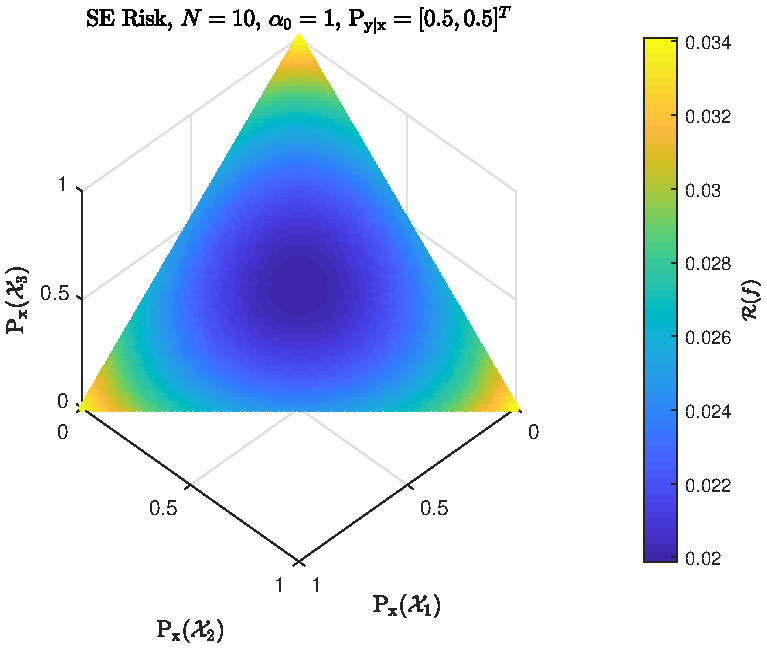
\includegraphics[scale=1.0]{Risk_SE_Dir_IO_Px_N_10_a0_1.pdf}
\caption{Optimal SE Risk for different PMF's $\Prm(\xrm)$}
\label{fig:Risk_SE_Dir_IO_Px_N_10_a0_1}
\end{figure}

\begin{figure}
\centering
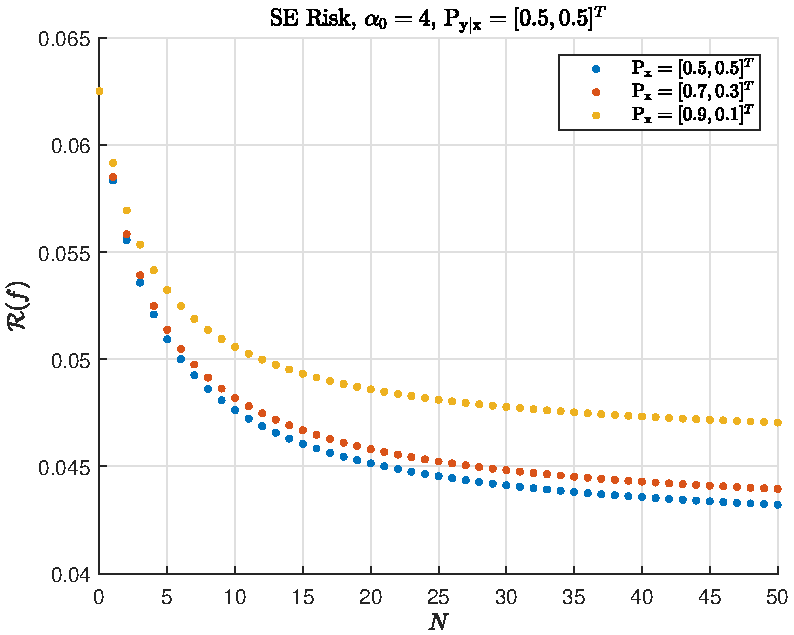
\includegraphics[scale=1.0]{Risk_SE_Dir_IO_N_leg_Px.pdf}
\caption{Optimal SE Risk for different training set sizes $N$}
\label{fig:Risk_SE_Dir_IO_N_leg_Px}
\end{figure}

\begin{figure}
\centering
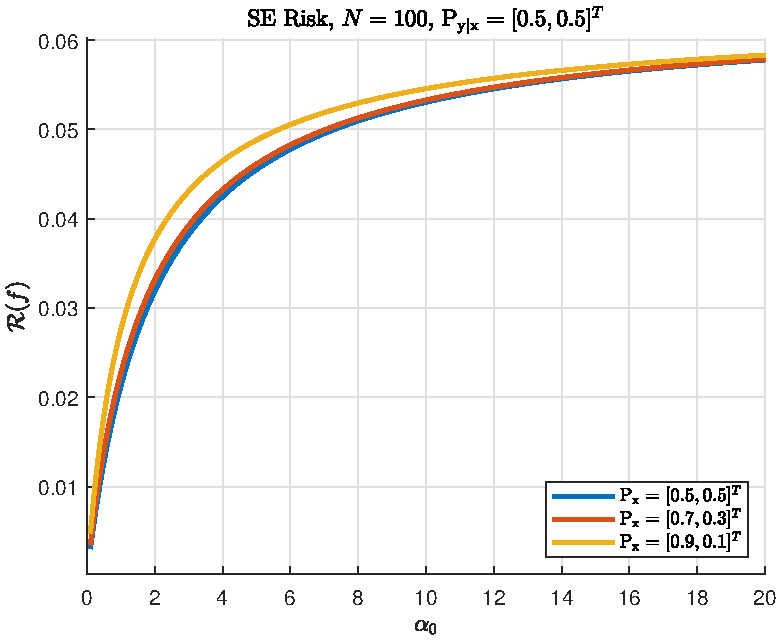
\includegraphics[scale=1.0]{Risk_SE_Dir_IO_a0_leg_Px.pdf}
\caption{Optimal SE Risk for different prior concentrations $\alpha_0$}
\label{fig:Risk_SE_Dir_IO_a0_leg_Px}
\end{figure}




\subparagraph{Uniform Prior}

For the uniform model prior, the risk reduces to
\begin{IEEEeqnarray}{rCl}
\Rcal(f^*) & = & \frac{|\Ycal| \big( N/|\Xcal| + |\Ycal| + 1 \big)}{\big( |\Ycal| + 1 \big) \big( N/|\Xcal| + |\Ycal| \big)} \\
&& \quad \left[ \left( \frac{1}{|\Ycal|} \sum_{y \in \Ycal} y^2 \right) - \left( \frac{1}{|\Ycal|} \sum_{y \in \Ycal} y \right)^2 \right] \nonumber \\
& = & \frac{1 + \big( N/|\Xcal| + |\Ycal| \big)^{-1}}{1 + |\Ycal|^{-1}} \left[ \left( \frac{1}{|\Ycal|} \sum_{y \in \Ycal} y^2 \right) - \left( \frac{1}{|\Ycal|} \sum_{y \in \Ycal} y \right)^2 \right] \nonumber \;.
\end{IEEEeqnarray}
Since all possible values of $\xrm$ are equally probable and the conditional probability $\Prm(\yrm|\xrm)$ is uniform and independent of $\xrm$, the risk simply becomes the variance of the set $\Ycal$ scaled by a factor dependent on $|\Ycal|$ and on $N/|\Xcal|$. Without training data ($N=0$), the scaling is unity; as $N/|\Xcal| \to \infty$, the scaling factor is $\big( 1 + |\Ycal|^{-1} \big)^{-1}$.

To visualize the performance, use the explicit sets $\Ycal$ and $\Xcal$ defined earlier. The conditional variance becomes
\begin{equation}
\Sigma_{\yrm | \xrm} = \frac{|\Ycal|^2 - 1}{12 |\Ycal|^2} = \frac{1 - |\Ycal|^{-2}}{12} 
\end{equation}
and the minimum risk is expressed as
\begin{IEEEeqnarray}{rCl}
\Rcal(f^*) & = & \frac{\big(1 - |\Ycal|^{-1}\big) \Big(1 + \big(N/|\Xcal| + |\Ycal|\big)^{-1} \Big)}{12} \\
& = & \left(\frac{|\Ycal|}{N/|\Xcal| + |\Ycal|}\right) \frac{1 - |\Ycal|^{-2}}{12} \nonumber \\
&& \quad + \left(\frac{N/|\Xcal|}{N/|\Xcal| + |\Ycal|}\right) \frac{1 - |\Ycal|^{-1}}{12} \nonumber \;.
\end{IEEEeqnarray}

Interestingly, the minimum squared-error for the uniform prior can be represented as a convex combination of two separate risk values with weighting factors dependent on $|\Ycal|$ and $N/|\Xcal|$. Thus for a uniform prior, the risk depends on the number of elements in $\Ycal$ and the number of training samples ``per element of $\Xcal$''. Note the relationship of these weighting factors to those of the conditional PMF $\Prm(\yrm | \xrm,\Drm)$, which depend on $\alpha'(\xrm)$ and on $N'(\xrm;\Drm)$. For the uniform prior, $\alpha'(\xrm) = |\Ycal|$ and $\Erm\big[ N'(\Drm) \big] = N/|\Xcal|$.

The first risk is the conditional variance $\Sigma_{\yrm|\xrm}$ - this is intuitively satisfying as the corresponding weight becomes unity when $N=0$. The second risk is the squared-error with infinite training data. Note that the reduction of the risk between these two extreme cases is modest, and that the attenuating factor increases towards unity for applications with more possible outcomes. Figure \ref{fig:Risk_SE_uniform_N_lim} illustrates the difference between these cases.

\begin{figure}
\centering
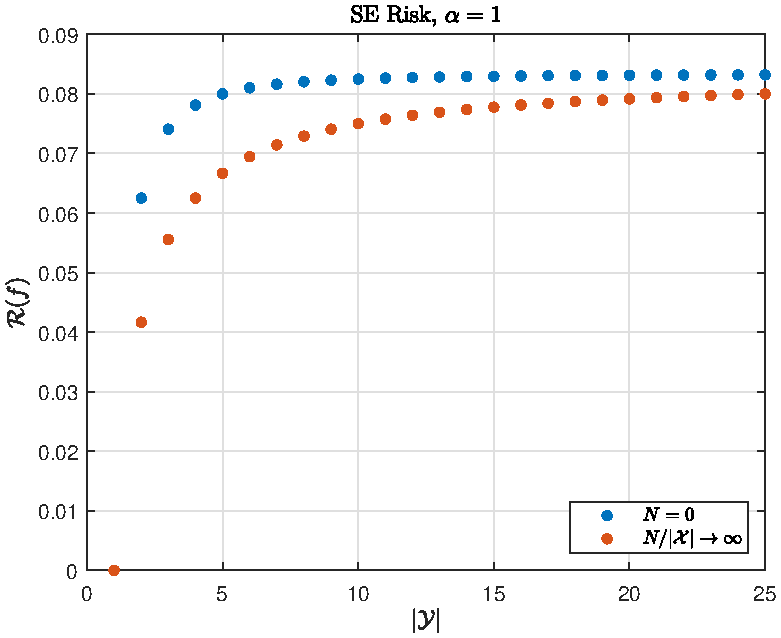
\includegraphics[scale=1.0]{Risk_SE_uniform_N_lim.pdf}
\caption{Optimal SE Risk, Uniform Prior, zero and infinite training data}
\label{fig:Risk_SE_uniform_N_lim}
\end{figure}


PGR: additional figures for uniform case?

%Figure \ref{fig:Risk_SE_IO_N} displays how the risk increases with $M_x$; Figure \ref{fig:Risk_SE_IO_N-Mx} makes the dependency on $N/M_x$ explicit.
%
%\begin{figure}
%\centering
%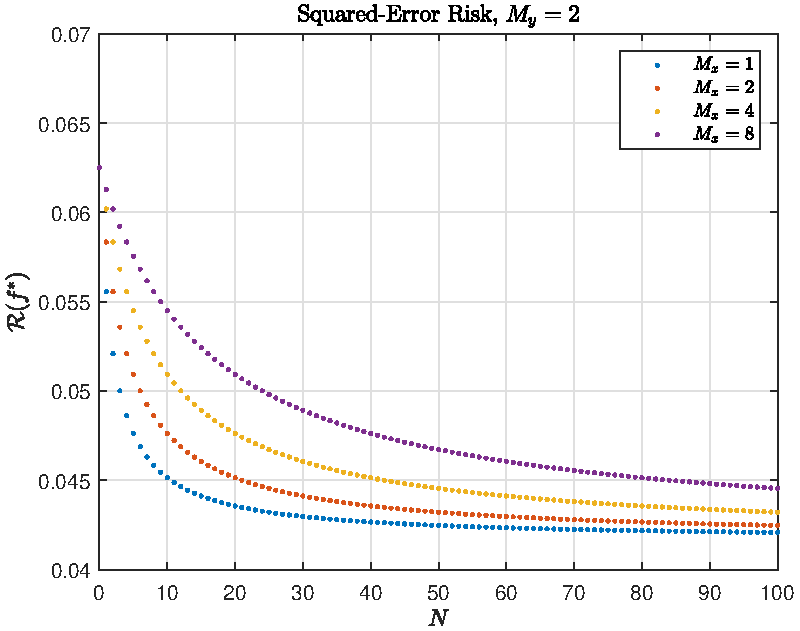
\includegraphics[scale=1.0]{Risk_SE_IO_N.pdf}
%\caption{Optimal SE Risk for different $|\Xcal|$, Uniform Prior}
%\label{fig:Risk_SE_IO_N}
%\end{figure}
%
%\begin{figure}
%\centering
%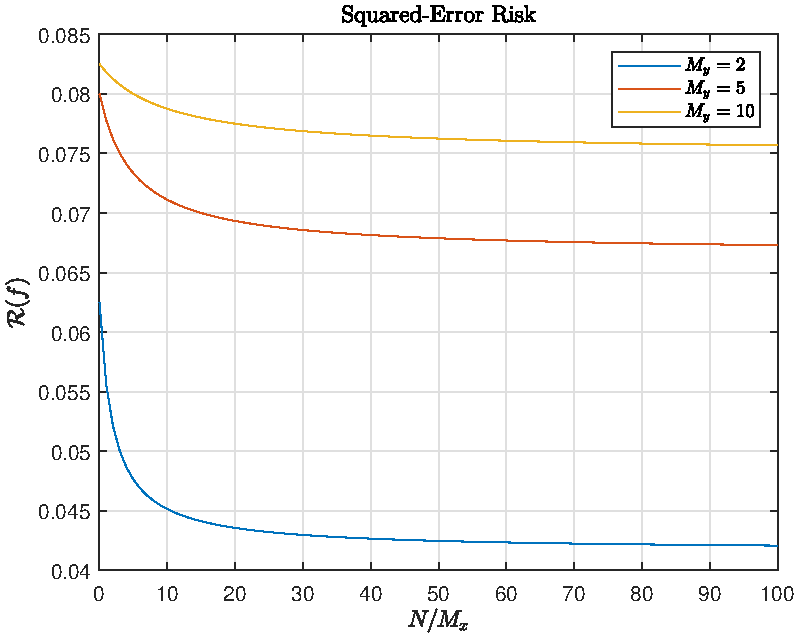
\includegraphics[scale=1.0]{Risk_SE_IO_N-Mx.pdf}
%\caption{Optimal SE Risk vs $N/|\Xcal|$, Uniform Prior}
%\label{fig:Risk_SE_IO_N-Mx}
%\end{figure}














\newpage

\section{Applications 01 temp}


\subsection{0-1 Loss}

In this section, we will apply the developed framework to a common machine learning task: classification. In classification problems, the unobserved variable space is countable and typically finite. Furthermore, the hypothesis space  is usually identical to the unobserved variable space, that is $\Hcal = \Ycal$. The 0-1 loss function is the most well known for these problems; it is represented as
\begin{equation} \label{loss_01}
\mathcal{L}(h,y) = 1 - \delta[h,y] \;.
\end{equation}

Applying this loss function, the conditional risk \eqref{eq:risk_cond} is
\begin{IEEEeqnarray}{rCl}
\Rcal_{\Theta}(f ; \theta) & = & 1 -  \Erm_{\Drm | \theta} \bigg[ \Erm_{\yrm,\xrm | \theta} \Big[ \delta\big[ f(\xrm;\Drm),\yrm \big] \Big] \bigg] \\
& = & 1 -  \sum_{x \in \Xcal} \Erm_{\Drm | \theta} \Big[ \theta\big( f(x,\Drm),x \big) \Big] \nonumber \;.
\end{IEEEeqnarray}
Evaluated with a Dirichlet prior, the full risk is
\begin{IEEEeqnarray}{rCl} \label{eq:risk_01}
\Rcal(f) & = & 1 - \Erm_{\theta} \left[ \sum_{x \in \Xcal} \Erm_{\Drm | \theta} \Big[ \theta\big( f(x,\Drm),x \big) \Big] \right] \\
& = & 1 - \sum_{x \in \Xcal} \frac{\Erm_{\Drm} \Big[ \alpha\big( f(x,\Drm),x \big) + \bar{N}\big( f(x,\Drm),x ; \Drm \big) \Big]}{\alpha_0 + N} \nonumber \\
& = & 1 - \sum_{x \in \Xcal} \frac{\Erm_{\nbarrm} \Big[ \alpha\big( f(x,\nbarrm),x \big) + \bar{\nrm}\big( f(x,\nbarrm),x \big) \Big]}{\alpha_0 + N} \nonumber \;.
\end{IEEEeqnarray}



\subsubsection{Optimal Hypothesis: Conditional Maximum \emph{a posteriori}}

PGR: decision region figures??

To determine the optimal learning function, substitute the 0-1 loss from Equation \eqref{loss_01} into Equation \eqref{eq:E_y|xD L} and Equation \eqref{eq:f_opt_xD} to find
\begin{IEEEeqnarray}{rCl} \label{eq:f_opt_01}
f^*(\xrm;\Drm) & = & \argmin_{h \in \Ycal} \frac{\sum_{y \in \Ycal} \big( \alpha(y,\xrm) + \bar{N}(y,\xrm;\Drm) \big) \big( 1 - \delta[h,y] \big)}{\alpha'(\xrm) + N'(\xrm;\Drm)} \\
& = & \argmax_{h \in \Ycal} \Prm_{\yrm | \xrm,\Drm}(h | \xrm,\Drm) \nonumber \\
& = & \argmax_{y \in \Ycal} \left( \alpha(y,\xrm) + \bar{N}(y,\xrm;\Drm) \right) \nonumber \;.
\end{IEEEeqnarray}
The optimal classifier chooses the value $\yrm$ that has the maximum value in the conditional PMF for the observed value of $\xrm$; each candidate decision $h \in \Ycal$ is scored by counting the number of training samples that occur with the same observed value as $\xrm$ and weighting with the prior knowledge imparted by the model parameter $\alpha$.


\paragraph{Uniform Prior}

When the uniform prior is used, the decision becomes 
\begin{IEEEeqnarray}{rCl}
f^*(\xrm;\Drm) & = & \argmax_{y \in \Ycal} \bar{N}(y,\xrm;\Drm) \;,
\end{IEEEeqnarray}
a majority decision which simply chooses the class from $\Ycal$ most often found among training set samples $\Drm$ with a matching input value $\xrm$. This is intuitive, as the model PDF parameter $\alpha$ provides no confidence as to which classes may be most likely.


\subsubsection{Minimum Risk: Probability of Error}

Substituting the optimal learner \eqref{eq:f_opt_01} into the general risk \eqref{eq:risk_01}, the minimum probability of error is 
\begin{IEEEeqnarray}{rCl}
\Rcal(f^*) & = & 1 - \Erm_{\xrm,\Drm} \left[ \max_{y \in \Ycal} \Prm_{\yrm | \xrm,\Drm}(y | \xrm,\Drm) \right] \\
& = & 1 - \sum_{x \in \Xcal} \frac{\Erm_{\nbarrm} \Big[ \max_{y \in \Ycal} \big( \alpha(y,x) + \bar{\nrm}(y,x) \big) \Big]}{\alpha_0 + N} \nonumber \;.
\end{IEEEeqnarray}

PGR: missing info for Dir gen graphics? fixed y given x conditional alpha???

PGR: no closed-forms found???


PGR: comment on simulation!

For $N = 0$, we have $\Rcal(f^*) = 1 - \sum_{x \in \Xcal} \frac{\max_{y \in \Ycal} \alpha(y,x)}{\alpha_0}$. 

For $N \to \infty$, we have $\Rcal(f^*) = ???$.

For $\alpha_0 \to 0$ and $N > 1$, we have $\Rcal(f^*) = 0$. Refer to \ref{eq:P_n_lim_zero}

For $\alpha_0 \to \infty$, we have $\Rcal(f^*) = 1 - \sum_{x \in \Xcal} \frac{\max_{y \in \Ycal} \alpha(y,x)}{\alpha_0}$.



\begin{figure}
\centering
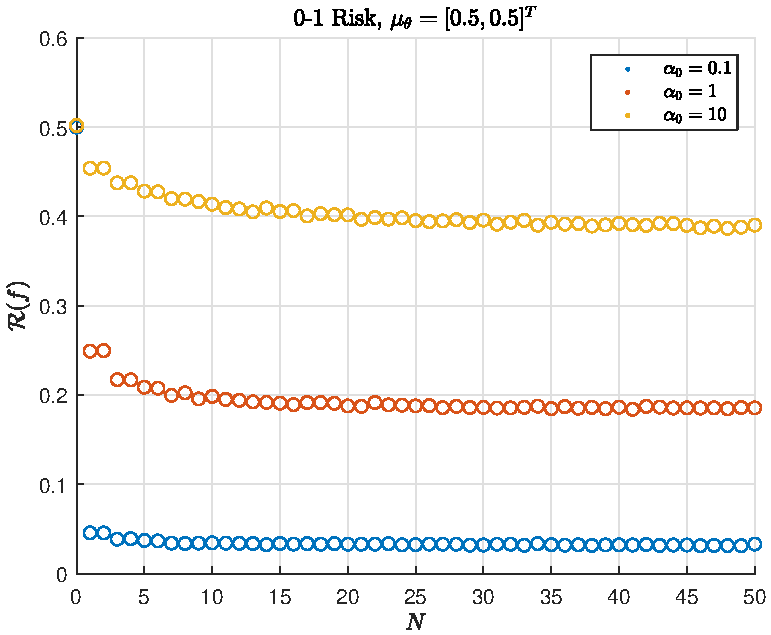
\includegraphics[scale=1.0]{Risk_01_Dir_N.pdf}
\caption{Optimal 0-1 Risk vs $N$}
\label{fig:Risk_01_Dir_N}
\end{figure}

\begin{figure}
\centering
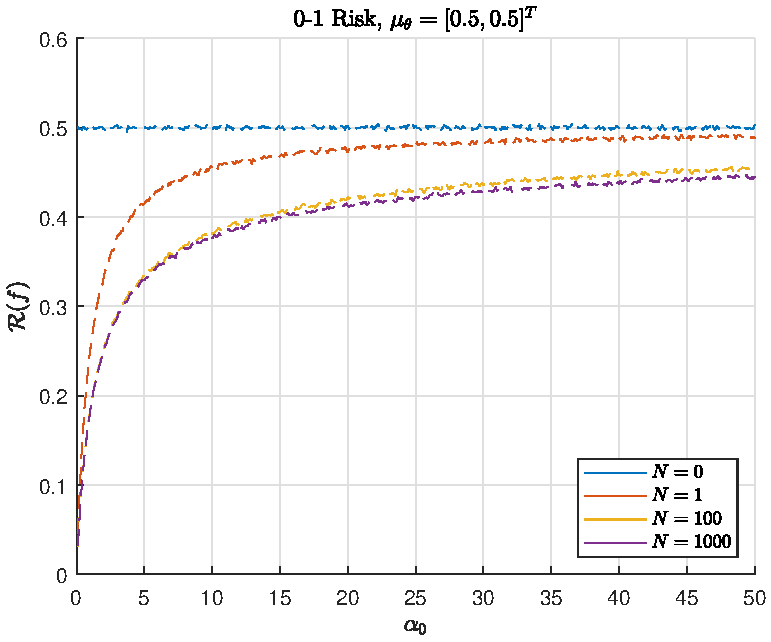
\includegraphics[scale=1.0]{Risk_01_Dir_alpha0.pdf}
\caption{Optimal 0-1 Risk vs $\alpha_0$}
\label{fig:Risk_01_Dir_alpha0}
\end{figure}

\begin{figure}
\centering
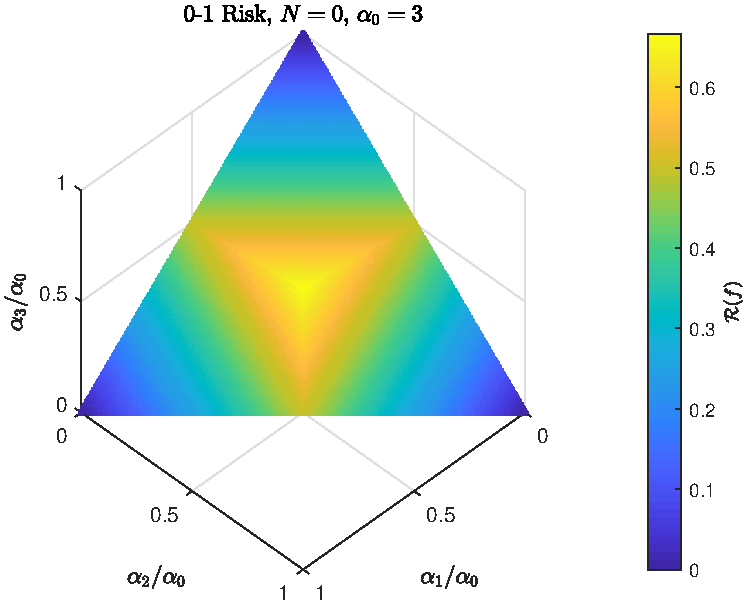
\includegraphics[scale=1.0]{Risk_01_Dir_muTheta_N_0_a0_3.pdf}
\caption{Optimal 0-1 Risk vs $\mu_{\theta}$}
\label{fig:Risk_01_Dir_muTheta_N_0_a0_3}
\end{figure}

\begin{figure}
\centering
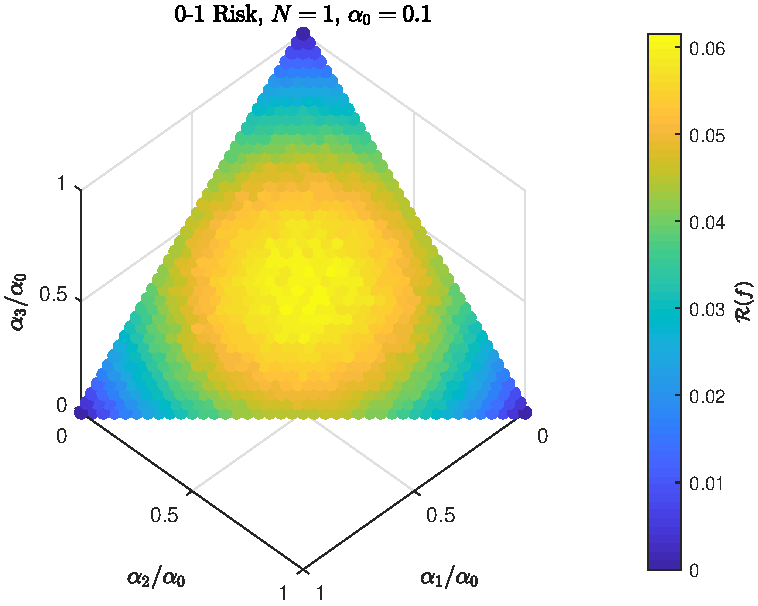
\includegraphics[scale=1.0]{Risk_01_Dir_muTheta_N_1_a0_01.pdf}
\caption{Optimal 0-1 Risk vs $\mu_{\theta}$}
\label{fig:Risk_01_Dir_muTheta_N_1_a0_01}
\end{figure}

\begin{figure}
\centering
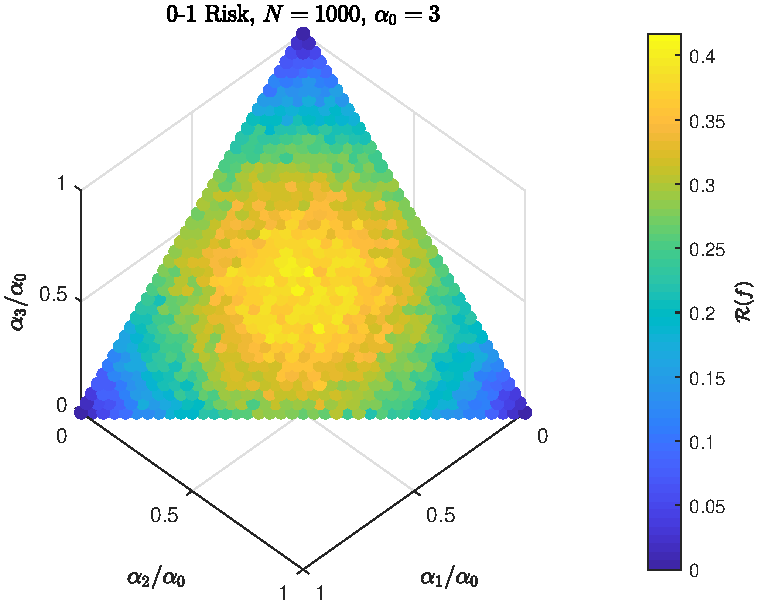
\includegraphics[scale=1.0]{Risk_01_Dir_muTheta_N_1000_a0_3.pdf}
\caption{Optimal 0-1 Risk vs $\mu_{\theta}$}
\label{fig:Risk_01_Dir_muTheta_N_1000_a0_3}
\end{figure}


\begin{figure}
\centering
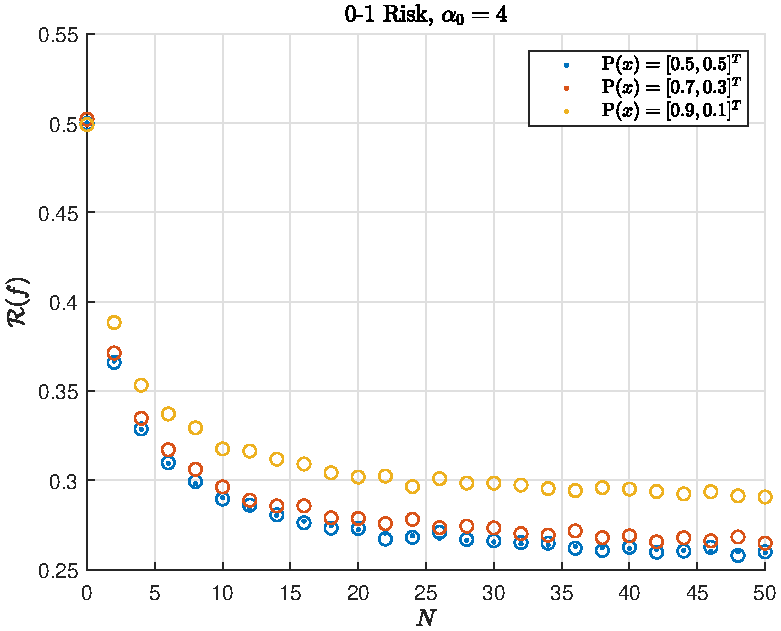
\includegraphics[scale=1.0]{Risk_01_Dir_IO_N_leg_Px.pdf}
\caption{Optimal 0-1 Risk vs $N$}
\label{fig:Risk_01_Dir_IO_N_leg_Px}
\end{figure}

\begin{figure}
\centering
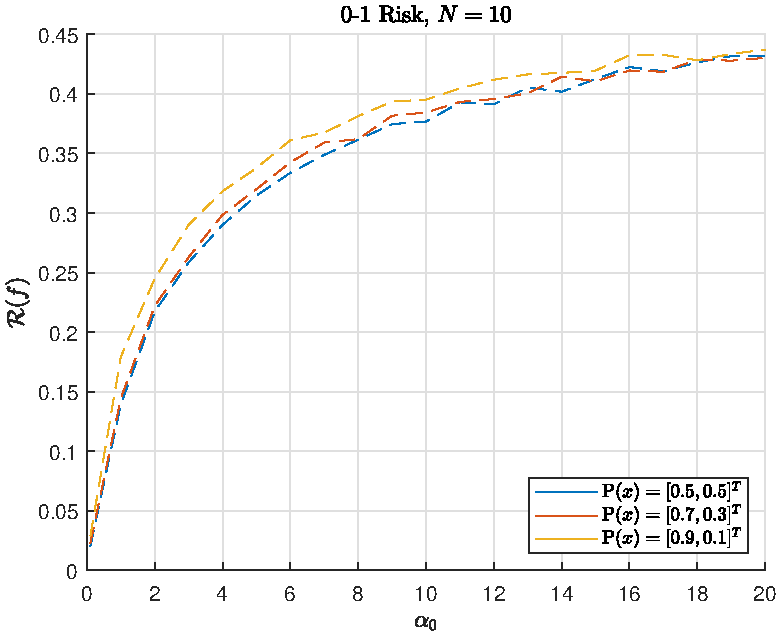
\includegraphics[scale=1.0]{Risk_01_Dir_IO_a0_leg_Px.pdf}
\caption{Optimal 0-1 Risk vs $\alpha_0$}
\label{fig:Risk_01_Dir_IO_a0_leg_Px}
\end{figure}

\begin{figure}
\centering
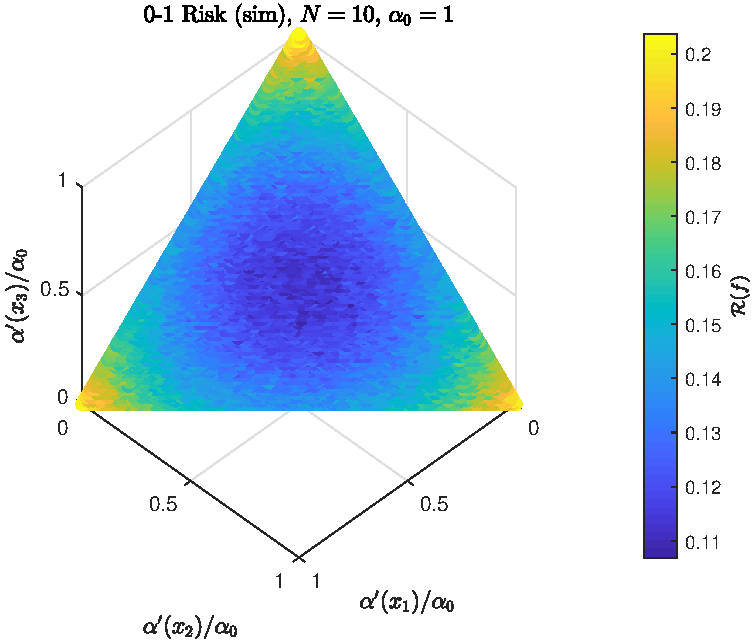
\includegraphics[scale=1.0]{Risk_01_Dir_IO_Px_N_10_a0_1.pdf}
\caption{Optimal 0-1 Risk vs $\Prm(x)$}
\label{fig:Risk_01_Dir_IO_Px_N_10_a0_1}
\end{figure}



\paragraph{Uniform Prior}

PGR: Can uniform optimal risk be approximated as a function of My and Mx/N, as is for SE loss???

To assess the minimum risk under the general model, we start from equation \eqref{risk_min_IO} and rework the formula to depend on an expectation over $\Prm(\Drm)$ as performed orginally, resulting in
\begin{IEEEeqnarray}{rCl}
\Rcal(f^*) & = & \Erm_{\xrm,\Drm} \bigg[ \Erm_{\yrm | \xrm,\Drm} \Big[ \mathcal{L}\big( f^*(\xrm;\Drm),\yrm \big) \Big] \bigg] \\
& = & 1 - \Erm_{\xrm,\Drm} \left[ \max_{y} \Prm_{\yrm | \xrm,\Drm}(y | \xrm,\Drm) \right] \nonumber \\
& = & 1 - \sum_{x \in \Xcal} \Erm_{\Drm} \left[ \max_{y} \Prm_{\yrm,\xrm | \Drm}(y,x | \Drm) \right] \nonumber \\
& = & 1 - \frac{\sum_{x \in \Xcal} \Erm_{\Drm} \left[\max_{y} \bar{N}(y,x;\Drm) \right] + 1}{N+M} \nonumber \;.
\end{IEEEeqnarray}

Now, however, the argument of expectation is the maximum of a subset of $\bar{N}(\Drm)$, $M_y$ out of $M_xM_y$, rather than the entire random variable. As shown in Appendix \ref{app:E_N_bar}, all marginal distributions of $\nbarrm$ have the same form; as such, the expectations will be the same regardless of which $M_y$ variables the maximum operator is applied to. 

To evaluate the expectation for an abritrary value $x$, we find a formula for the CMF of the maximum of any $k$ of $M$ entries of random matrix $\nbarrm$. Introduce subset $\Ycal' \subset \Ycal$ with cardinality $k$. Denote the new variable as $\bar{\nrm}_{\mathrm{max}}^k \equiv \max_{y \in \Ycal'} \bar{\nrm}(y)$; we find in Appendix ??? that the CMF is equivalent to
\begin{IEEEeqnarray}{rCl}
F_{\bar{\nrm}_{\mathrm{max}}^k}(n) & = & \Prm\big( \bar{\nrm}_{\mathrm{max}}^k \leq n \big) \\
& = & \sum_{m=0}^k \binom{k}{m} (-1)^m \prod_{l=1}^{M-1} \left( 1 - \frac{m(n+1)}{N+l} \right) \nonumber \\
&& \quad  \left[ U(n) - U\left( n+1- \left\lceil \frac{N+M}{m} \right\rceil \right) \right] \nonumber \;.
\end{IEEEeqnarray}
Evaluating the expectation, we have
\begin{IEEEeqnarray}{rCl}
\Erm_{\bar{n}} \left[ \bar{\nrm}_{\mathrm{max}}^k \right] & = & N+M - \sum_{n=0}^{N+M-1} F_{\bar{\nrm}_{\mathrm{max}}^k}(n) \\
& = & - \sum_{m=1}^k \binom{k}{m} (-1)^m \left[ \sum_{n=1}^{N+M} \prod_{l=1}^{M-1} \left( 1 - \frac{mn}{N+l} \right) - \sum_{n=\left\lceil \frac{N+M}{m} \right\rceil}^{N+M} \prod_{l=1}^{M-1} \left( 1 - \frac{mn}{N+l} \right) \right] \nonumber \;.
%& = & sumbounds??? - \sum_{m=1}^k \binom{k}{m} (-1)^m \sum_{n=1}^{\left\lceil \frac{N+M}{m} \right\rceil -1} \prod_{l=1}^{M-1} \left( 1 - \frac{mn}{N+l} \right) \;.
\end{IEEEeqnarray}
Making use of the summation identity
\begin{equation}
\sum_{m=0}^k \binom{k}{m} (-1)^m = 0 \;,
\end{equation}
we substitute in to the formula for minimum risk using $k=M_y$, resulting in
\begin{IEEEeqnarray}{rCl}
\Rcal(f^*) & = & 1 + \frac{M_x}{N+M} \sum_{m=1}^{M_y} \binom{M_y}{m} (-1)^m \sum_{n=0}^{\left\lceil \frac{N+M}{m} \right\rceil -1} \prod_{l=1}^{M-1} \left( 1 - \frac{mn}{N+l} \right) \;.
\end{IEEEeqnarray}

PGR: Proof? CHECK....???



Figure \ref{fig:Risk_01_IO_N} displays how the optimal risk decreases with increasing training data; the number of outputs is fixed at $M_y = 2$ and multiple series are provided for different input set sizes $M_x$. The plot for $M_x = 1$ is obviously identical to the series shown in Section \ref{sec:uniform_basic_apps_01}. For larger input set sizes, the risk is still $\Rcal(f^*) = 0.5$ when $N = 0$, but the rate of decrease with $N$ suffers. 

\begin{figure}
\centering
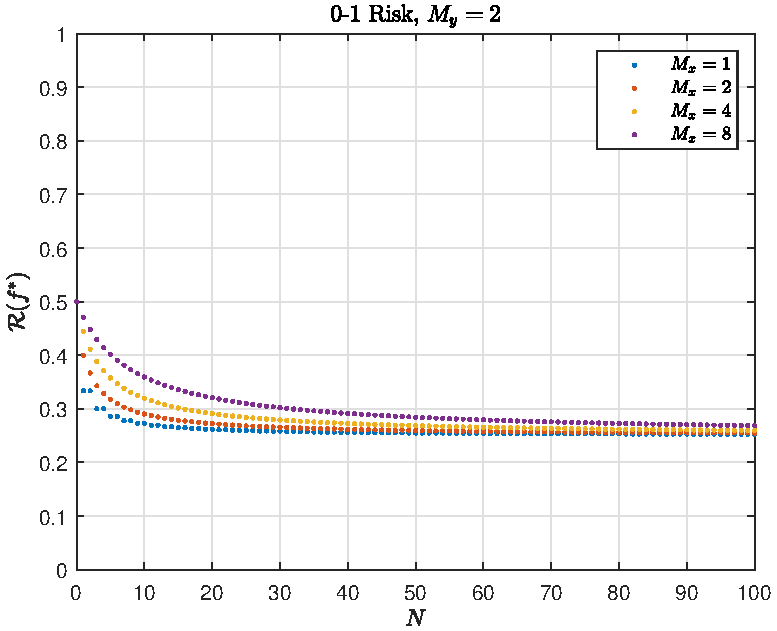
\includegraphics[scale=1.0]{Risk_01_IO_N.pdf}
\caption{Optimal 0-1 Risk vs training set size for various input set sizes}
\label{fig:Risk_01_IO_N}
\end{figure}

Further insight into how $M_x$ affects the risk can be acquired by plotting the risk vs $N/M_x$. In Figure \ref{fig:Risk_01_IO_N-Mx}, it is shown that the optimal risk can be approximated by a function dependent only on $N/M_x$; of the series plotted, only the series for $M_x = 1$ shows notable deviation from the others.

\begin{figure}
\centering
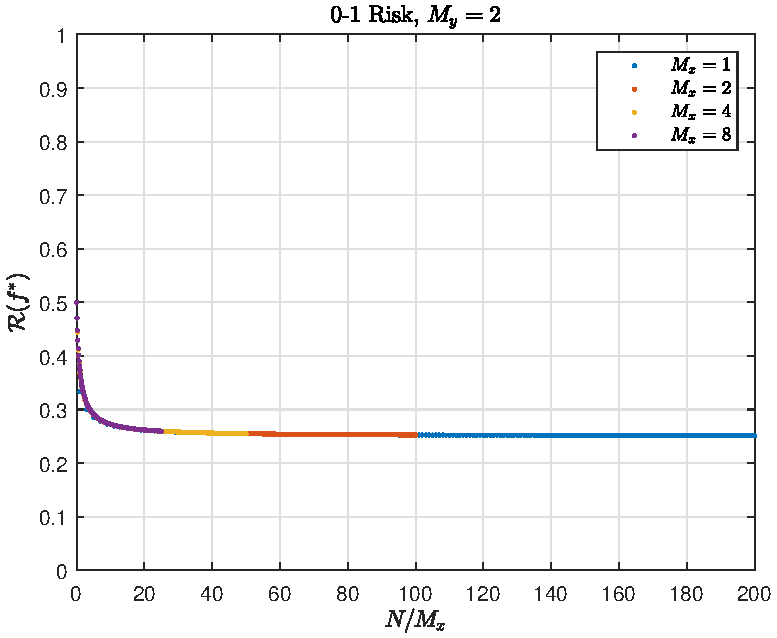
\includegraphics[scale=1.0]{Risk_01_IO_N-Mx.pdf}
\caption{Optimal 0-1 Risk vs training set size for various input set sizes}
\label{fig:Risk_01_IO_N-Mx}
\end{figure}



As for the basic model, it is informative to note how the minimum risk trends with increasing volume of training data. Noting that
\begin{IEEEeqnarray}{rCl}
\lim_{N \to \infty} (N+M)^{-1} \sum_{n=0}^{\left\lceil \frac{N+M}{m} \right\rceil -1} \prod_{l=1}^{M-1} \left( 1 - \frac{mn}{N+l} \right) & = & \\
\lim_{N/m \to \infty} m^{-1} \frac{m}{N} \sum_{n=0}^{\left\lceil \frac{N}{m} \right\rceil -1} \left( 1 - \frac{mn}{N} \right)^{M-1} & = & \nonumber \\
m^{-1} \int_0^1 (1-t)^{M-1} \mathrm{d} t & = & \frac{1}{mM} \nonumber \;,
\end{IEEEeqnarray}
and using the same concepts from Appendix \ref{app:E_N_max}, we find
\begin{IEEEeqnarray}{rCl}
\Rcal(f^*) & = & 1 + \frac{M_x}{M} \sum_{m=1}^{M_y} \binom{M_y}{m} (-1)^m m^{-1} \\
& = & 1 - \frac{1}{M_y} \sum_{m=1}^{M_y} \frac{1}{m} \nonumber \;.
\end{IEEEeqnarray}

%\begin{IEEEeqnarray}{rCl}
%1 - \Rcal(f^*) & = & -\frac{M_x}{M} \sum_{m=1}^{M_y} \binom{M_y}{m} (-1)^m m^{-1} \\
%& = & \frac{1}{M_y} \sum_{m=1}^{M_y} \frac{1}{m} \;.
%\end{IEEEeqnarray}

Again, we have a harmonic number dependent on the number of possible outputs $M_y$. With infinite training data, there will be an infinite number of samples for each possible input $\xrm$; as a result, there is no loss of classification performance regardless of the input dimension $M_x$. This agrees with the notion that optimal 0-1 risk can be approximated as a function of $N/M_x$.























\section{Applications: basic uniform}



\subsection{Classification: the 0-1 Loss} \label{sec:uniform_basic_apps_01}

\subsubsection{Minimum Risk: the Probability of Error}
Now, we determine the minimum risk (probability of error for the 0-1 loss). Starting from equation \eqref{risk_min}, we formulate the risk as
\begin{IEEEeqnarray}{rCl} \label{risk_01_opt}
\Rcal(f^*) & = & \Erm_{\Drm} \Big[ \Erm_{\yrm | \Drm} \big[ \mathcal{L}(f^*(\Drm),\yrm) \big] \Big]
= 1 - \Erm_{\Drm} \left[ \max_{y} \Prm_{\yrm | \Drm}(y | \Drm) \right] \\
& = & 1 - \Erm_{\Drm} \left[ \frac{\max_{y \in \Ycal} \bar{N}(y;\Drm) + 1}{N+M} \right] \nonumber \\
& = & 1 - \left( \frac{M}{N+M} \right) M^{-1} - \left( \frac{N}{N+M} \right) \frac{\Erm_{\Drm} \left[ \max_{y \in \Ycal} \bar{N}(y;\Drm) \right]}{N} \nonumber \;. 
\end{IEEEeqnarray}

Before refining this expression, observe how the minimum risk trends as $M$ increases for fixed training set size $N$. Clearly, $\lim_{M \to \infty} \Rcal(f^*) = 1 - M^{-1}$. This should be intuitively satisfying -- the posterior PMF trends toward a discrete uniform distribution, the same as if no data had been observed at all (e.g. $\Prm(\yrm) = M^{-1}$).

Next, we continue to find a closed-form expression for the optimal risk; to do so, we must evaluate the expectation over all possible training sets $\Drm$. It can be clearly shown that the expectation can instead be performed over random variable $\nbarrm = \bar{N}(\Drm)$, that is,
\begin{equation}
\Erm_{\Drm} \left[ \max_y \bar{N}(y;\Drm) \right] = \Erm_{\nbarrm} \left[ \max_y \bar{\nrm}(y) \right] \;.
\end{equation}

In Appendix \ref{app:E_N_max}, we determine the cumulative mass function (CMF) of $\bar{\nrm}_{\mathrm{max}} = \max_y \bar{\nrm}(y)$, 
\begin{IEEEeqnarray}{rCl}
F_{\bar{\nrm}_{\mathrm{max}}}(n) & = & \Prm\left( \bar{\nrm}_{\mathrm{max}} \leq n \right) \\
& = & \binom{N+M-1}{M-1}^{-1} \sum_{m=1}^M \binom{M}{m} (-1)^{M-m} \nonumber \\
&& \quad \binom{m(n+1)-N-1}{M-1} U\left( n+1-\left\lceil\frac{N+M}{m}\right\rceil \right) \nonumber \;,
\end{IEEEeqnarray}
where $U: \Rbb \mapsto \{0,1\}$ is the continuous step function. Clearly, the PMF is zero outside of the interval $[0,N+M]$; the expected value is thus
\begin{IEEEeqnarray}{rCl}
\Erm_{\bar{n}} \left[ \bar{\nrm}_{\mathrm{max}} \right] & = & \sum_{n=0}^{N+M} n \big( F_{\bar{\nrm}_{\mathrm{max}}}(n) - F_{\bar{\nrm}_{\mathrm{max}}}(n-1) \big) \\
& = & N + M - \sum_{n=0}^{N+M-1} F_{\bar{\nrm}_{\mathrm{max}}}(n) \nonumber \\
& = & N + M - \binom{N+M-1}{M-1}^{-1} \sum_{m=1}^M \binom{M}{m} (-1)^{M-m} \nonumber \\
&& \quad \sum_{n = \left\lceil \frac{N+M}{m} \right\rceil}^{N+M} \binom{mn-N-1}{M-1} \nonumber \;.
\end{IEEEeqnarray}

This general equation has not been reduced to a more tractable form. Using it it conjunction with equation \eqref{risk_01_opt}, we have the expression for the optimal risk,
\begin{IEEEeqnarray}{rCl}
\Rcal(f^*) & = & 1 - \Erm_{\Drm} \left[ \frac{\max_y \bar{N}(y;\Drm) + 1}{N+M} \right] \\
& = & \frac{1}{N+M} \left[ -1 + \binom{N+M-1}{M-1}^{-1} \sum_{m=1}^M \binom{M}{m} (-1)^{M-m} \sum_{n = \left\lceil \frac{N+M}{m} \right\rceil}^{N+M} \binom{mn-N-1}{M-1}  \right] \nonumber \\
& = & \frac{-1}{N+M} \left[ 1 + \sum_{m=1}^M \binom{M}{m} (-1)^m \sum_{n = \left\lceil \frac{N+M}{m} \right\rceil}^{N+M} \prod_{l=1}^{M-1} \left( 1 - \frac{mn}{N+l} \right) \right] \nonumber \;.
%& = & \frac{M - 1 +\binom{N+M-1}{M-1}^{-1} \sum_{m=1}^M \binom{M}{m} (-1)^{M-m} \sum_{n = \left\lceil \frac{N+M}{m} \right\rceil}^N \binom{mn-N-1}{M-1}}{N+M} \;.
\end{IEEEeqnarray}
Figure \ref{fig:Risk_01_vsN} displays the risk as a function of $N$ for select values of $M$. Observe that even for binary classification, the optimal risk asymptotes quickly.

PGR: Havent found closed form for summation over n. Can a bound be found instead???

\begin{figure}
\centering
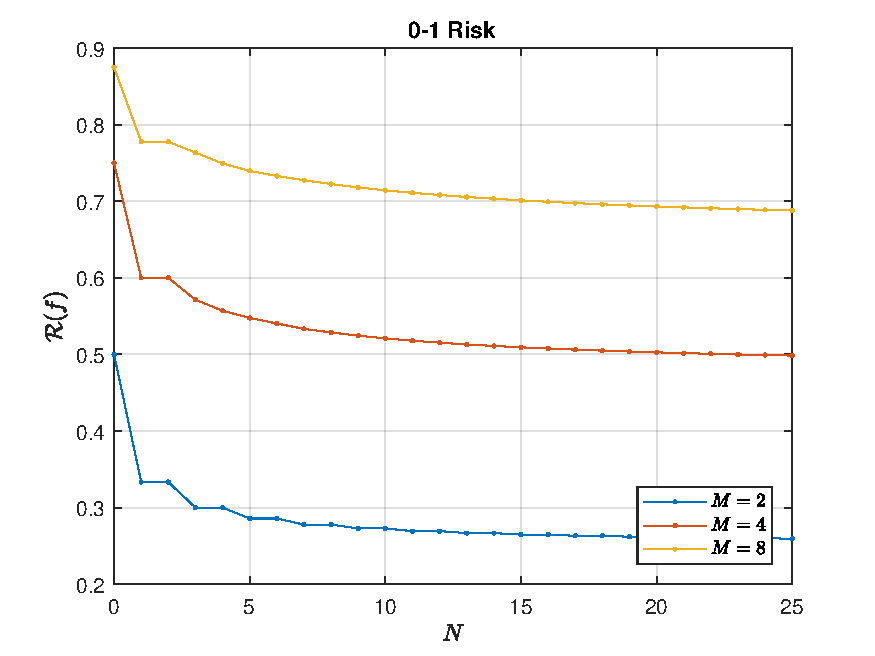
\includegraphics[scale=1.0]{Risk_01_vsN.pdf}
\caption{Optimal 0-1 Risk, vs. Training Set volume $N$}
\label{fig:Risk_01_vsN}
\end{figure}

The performance of this optimal decision function in the limit of training set volume $N \to \infty$ is of interest. Fortunately, the expectation $\Erm_{\bar{\bm{\mathrm{n}}}} \big[ \max_y \bar{\nrm}(y) \big]$ can be represented more compactly in this limit. As detailed in Appendix \ref{app:E_N_max},
\begin{equation}
\lim_{N \to \infty} \frac{\Erm_{\bar{\bm{\mathrm{n}}}} \big[ \max_y \bar{\nrm}(y) \big]}{N} = \frac{1}{M} \sum_{m=1}^M \frac{1}{m} \;.
\end{equation}

Note that this summation has no closed-form -- it is a Harmonic number. Note also that if the class set is countably infinite, this summation can be represented as
\begin{IEEEeqnarray}{rCl}
\lim_{M \to \infty} \frac{1}{M} \sum_{m=1}^M \frac{1}{m} & = & \lim_{M \to \infty} \frac{\mathrm{ln}(M)}{M} \\
& = & \lim_{M \to \infty} \frac{1}{M} = 0 \nonumber \;.
\end{IEEEeqnarray}

PGR: harmonic reference???

Substituting the limiting form of the expectation into equation \eqref{risk_01_opt}, we determine the optimal risk
\begin{equation}
\lim_{N \to \infty} \Rcal(f^*)  = \lim_{N \to \infty} \left( 1 - \frac{\Erm_{\Drm} \left[ \max_y \bar{N}(y;\Drm) \right]}{N} \right) = 1 - \frac{1}{M} \sum_{m=1}^M \frac{1}{m} \;,
\end{equation}
which provides a lower bound to the risk that any learner can achieve with any volume of training data. Figure \ref{fig:Risk_01_LB} displays this risk, as well as the optimal risk when no training data is available. Note the margin in the probability of error between the optimal $N=0$ and $N \to \infty$ learners. For binary classification (the simplest case), we see a modest reduction from 0.5 to 0.25 error; for higher values of $M$, the probability of error increases towards unity. Clearly, this level of error is unacceptable for most applications. Nonetheless, it is the minimum risk for the problem we have formulated -- this results from our choosing a non-informative prior over $\Theta$.

\begin{figure}
\centering
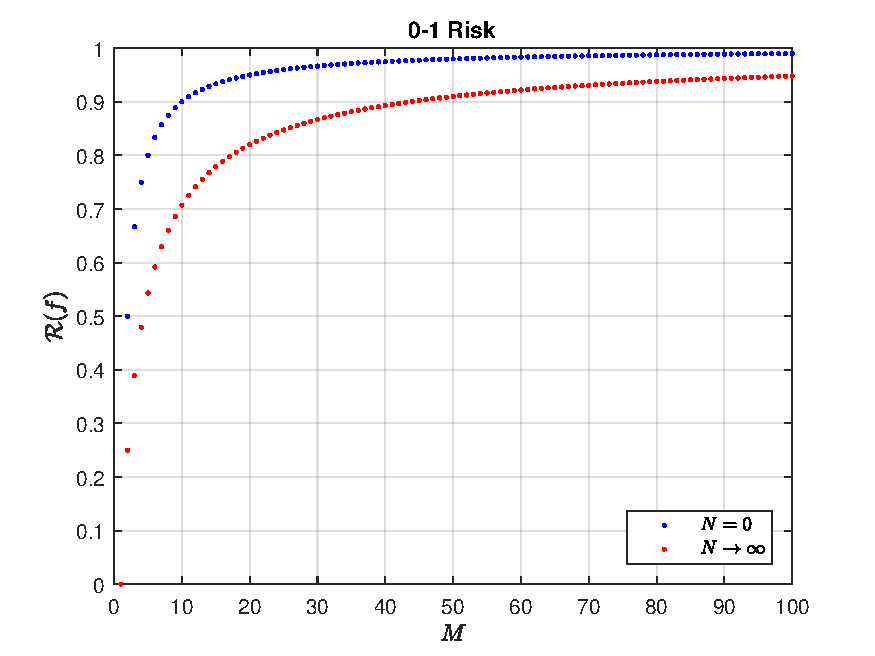
\includegraphics[scale=1.0]{Risk_01_LB.pdf}
\caption{Optimal 0-1 Risk, Upper and Lower bounds}
\label{fig:Risk_01_LB}
\end{figure}

PGR: PLOT RISK VS THETA???







































\newpage

\chapter{Extention to Infinite-Dimensional Spaces - Countably Infinite}

PGR: merge with finite chapter?

\section{Intro}

This chapter extends previous results for applications where the space $\Ycal$ can have an infinite number of elements. Specifically, the model distribution will be determined by using a Dirichlet random process prior. First, we assume that the set is countably infinite, that is $|\Ycal| = \aleph_0$; the model distribution is thus a discrete random process. 




\section{Basic Model}


\subsection{Probability Distributions}

PGR: ???


\subsubsection{Model PDF, $\prm(\theta)$}

PGR: Valid model representation? Marginals instead?


\begin{IEEEeqnarray}{rCl}
\prm(\theta) & = & \beta(\alpha)^{-1} \prod_{y \in \Ycal} \theta(y)^{\alpha(y) - 1} \;,
\end{IEEEeqnarray}

\begin{equation}
\beta(\alpha) = \frac{\prod_{y \in \Ycal} \Gamma\big( \alpha(y) \big)}{\Gamma \left( \sum_{y \in \Ycal} \alpha(y) \right)} \;.
\end{equation}

The first and second joint moments of the model are 
\begin{equation}
\mu_{\theta}(y) = \Erm_{\theta}\big[ \theta(y) \big] = \frac{\alpha(y)}{\alpha_0}
\end{equation}
and
\begin{IEEEeqnarray}{rCl}
\Erm_{\theta}\big[ \theta(y) \theta(y') \big] & = & \frac{\alpha(y) \alpha(y') + \alpha(y) \delta[y,y']}{\alpha_0 (\alpha_0+1)} \;.
\end{IEEEeqnarray}




\subsubsection{Training Data PMF, $\Prm(\Drm)$}

\begin{equation}
\Prm(\Drm | \theta) = \prod_{y \in \Ycal} \theta(y)^{\bar{N}(y;\Drm)} \;.
\end{equation}

\begin{equation}
\Prm(\nbarrm | \theta) = \Mcal(\nbarrm) \prod_{y \in \Ycal} \theta(y)^{\bar{\nrm}(y)} \;,
\end{equation}

Thus,
\begin{IEEEeqnarray}{rCl}
\Prm(\nbarrm) & = & \Mcal(\nbarrm) \beta(\alpha)^{-1} \beta(\alpha + \nbarrm) \;.
\end{IEEEeqnarray}

The first and second joint moments of $\nbarrm$ are
\begin{equation}
\Erm_{\bar{\nrm}}\big[ \bar{\nrm}(y) \big] = N \frac{\alpha(y)}{\alpha_0}
\end{equation}
and
\begin{equation}
\Erm_{\bar{\nrm}}\big[ \bar{\nrm}(y) \bar{\nrm}(y') \big] 
= \frac{N}{\alpha_0 (\alpha_0+1)} \big( (\alpha_0 + N)\alpha(y) \delta[y,y'] + (N-1) \alpha(y) \alpha(y') \big) \;.
\end{equation}

Also,
\begin{equation}
\Prm(\Drm) = \beta(\alpha)^{-1} \beta \big( \alpha + \bar{N}(\Drm) \big) \;.
\end{equation}






\subsubsection{Output conditional PMF, $\Prm(\yrm | \Drm)$}

\begin{IEEEeqnarray}{rCL}
\prm(\theta | \Drm) & = & \frac{\Prm(\Drm | \theta) \prm(\theta)}{\Prm(\Drm)} \\
& = & \beta \left( \alpha + \bar{N}(\Drm) \right)^{-1} \prod_{y \in \Ycal} \theta(y)^{\alpha(y) + \bar{N}(y;\Drm) - 1} \nonumber 
\end{IEEEeqnarray}

\begin{IEEEeqnarray}{rCL}
\prm(\theta | \nbarrm) = \beta \left( \alpha + \nbarrm \right)^{-1} 
\prod_{y \in \Ycal} \theta(y)^{\alpha(y) + \bar{\nrm}(y) - 1} \;,
\end{IEEEeqnarray}

The PMF of interest is
\begin{IEEEeqnarray}{rCl}
\Prm(\yrm | \Drm) & = & \Erm_{\theta | \Drm}\big[ \theta(\yrm) \big] \\
& = & \frac{\alpha(\yrm) + \bar{N}(\yrm;\Drm)}{\alpha_0 + N} \nonumber \\
& = & \left(\frac{\alpha_0}{\alpha_0+N}\right) \frac{\alpha(\yrm)}{\alpha_0} + \left(\frac{N}{\alpha_0+N}\right) \frac{\bar{N}(\yrm;\Drm)}{N} \nonumber
\end{IEEEeqnarray}

\begin{IEEEeqnarray}{rCl}
\Prm(\yrm | \nbarrm) & = & \Erm_{\theta | \nbarrm} \big[ \theta(\yrm) | \nbarrm \big] \\
& = & \frac{\alpha(\yrm) + \bar{\nrm}(\yrm)}{\alpha_0 + N} \nonumber \\
& = & \left(\frac{\alpha_0}{\alpha_0+N}\right) \frac{\alpha(\yrm)}{\alpha_0} + \left(\frac{N}{\alpha_0+N}\right) \frac{\bar{\nrm}(\yrm)}{N} \nonumber
\end{IEEEeqnarray}



\section{Application to Common Loss Functions}

PGR: Definitely regression. Classification sensible for countably infinite?

PGR: Results identical to finite Dirichlet

\begin{IEEEeqnarray}{L}
\Erm_{\yrm | \Drm} \big[ \mathcal{L}(h,\yrm) \big] = \sum_{y \in \Ycal} \mathcal{L}(h,y) \Prm_{\yrm | \Drm}(y | \Drm) \\
= \frac{\sum_{y \in \Ycal} \alpha(y) \mathcal{L}(h,y) + \sum_{y \in \Ycal} \bar{N}(y;\Drm) \mathcal{L}(h,y)}{\alpha_0+N} \nonumber \\
= \frac{\sum_{y \in \Ycal} \alpha(y) \mathcal{L}(h,y) + \sum_{n=1}^N \mathcal{L}\big( h,\Drm_n \big)}{\alpha_0+N} \nonumber \\
= \left( \frac{\alpha_0}{\alpha_0+N} \right) \sum_{y \in \Ycal} \mathcal{L}(h,y) \frac{\alpha(y)}{\alpha_0} +  \left( \frac{N}{\alpha_0+N} \right) N^{-1} \sum_{n=1}^N \mathcal{L}\big( h,\Drm_n \big) \nonumber \;.
\end{IEEEeqnarray}


\section{General Model}

Extension to output and input spaces $\Ycal$ and $\Xcal$ can have an infinite number of elements. 


\section{Applications: General Model}

PGR: Definitely regression. Classification sensible for countably infinite?

PGR: Results identical to finite Dirichlet












\chapter{Extention to Infinite-Dimensional Spaces - Uncountably Infinite}

PGR: SPECIFY EUCLIDEAN??

PGR: account for impulsive alpha?


\section{Intro}

This chapter extends further to the case where $\Ycal$ is uncountably infinite, that is $|\Ycal| \geq \aleph_1$; the model distribution is thus a continuous random process. 


\section{Basic Model}



\subsection{Probability Distributions}

PGR: ???


\subsubsection{Model $\theta$ Characterization}

The model is now a continuous random process, such that $\theta \sim \DP(\alpha)$. The concentration parameter is $\alpha_0 = \int_{y \in \Ycal} \alpha(y) \mathrm{d} y$. By definition, for any partition of the set $\Ycal$, $\left\{ \ldots,\Scal(z),\ldots \right\}$, $z \in \Zcal$, we can generate a discrete Dirichlet random vector/process $\phi(z) \equiv \int_{\Scal(z)} \theta(y) \mathrm{d} y$ with parameterizing function $\lambda(z) \equiv \int_{\Scal(z)} \alpha(y) \mathrm{d} y$. This is commonly referred to as the aggregation property. The PDF for the aggregation is thus
\begin{IEEEeqnarray}{rCl}
\prm(\phi) & = & \beta(\lambda)^{-1} \prod_{z \in \Zcal} \phi(z)^{\lambda(z) - 1} \;.
\end{IEEEeqnarray}

As detailed in Appendix \ref{app:E_DP}, the first and second moments of a Dirichlet process $\DP(\alpha)$ are
\begin{equation}
\mu_{\theta}(y) = \Erm\big[\theta(y)\big] = \frac{\alpha(y)}{\alpha_0}
\end{equation}
and
\begin{IEEEeqnarray}{rCl}
\Erm \big[ \theta(y) \theta(y') \big] & = & \frac{\alpha(y) \alpha(y') + \alpha(y) \delta(y-y')}{\alpha_0 (\alpha_0+1)} \;.
\end{IEEEeqnarray}







\subsubsection{Output conditional PDF, $\prm(\yrm | \Drm)$}

In Appendix \ref{app:DP_post}, it was shown that if the model $\theta \sim \DP(\alpha)$ is a Dirichlet process, then the model conditioned on the training data $\Drm$ is also a Dirichlet process with parameterizing function $\alpha + \bar{N}(\Drm)$, where $\bar{N}(y;\Drm) = \sum_{n=1}^N \delta\left( y - \Drm_n \right)$ generalizes from the discrete case. Thus, the conditional PDF of interest can be formulated as
\begin{IEEEeqnarray}{rCl}
\prm(\yrm | \Drm) & = & \Erm_{\theta | \Drm}\big[ \theta(\yrm) \big] \\
& = & \frac{\alpha(\yrm) + \sum_{n=1}^N \delta\big( \yrm - \Drm_n \big)}{\alpha_0 + N} \nonumber \\
& = & \left(\frac{\alpha_0}{\alpha_0+N}\right) \frac{\alpha(\yrm)}{\alpha_0} + \left(\frac{N}{\alpha_0+N}\right) \frac{\sum_{n=1}^N \delta\big( \yrm - \Drm_n \big)}{N} \nonumber \\
& = & \frac{\alpha(\yrm) + \bar{N}(\yrm;\Drm)}{\alpha_0 + N} \nonumber \;.
\end{IEEEeqnarray}
With the generalization to a continuous set $\Ycal$, the training data dependent component of the PDF is formulated with Dirac delta functions. 



\subsubsection{Training Data PDF, $\prm(\Drm)$}

To represent the training data distribution, note that the Dirichlet process conditional model also provides
\begin{IEEEeqnarray}{rCl}
\prm\big( \Drm_{n+1} | \Drm_n,\ldots,\Drm_1 \big) & = & \frac{\alpha\big( \Drm_{n+1} \big) + \sum_{i=1}^n \delta\big( \Drm_{n+1} - \Drm_i \big)}{\alpha_0 + N} \;
\end{IEEEeqnarray}
and thus the complete PDF is
\begin{IEEEeqnarray}{rCl}
\prm(\Drm) & = & \prm\big( \Drm_1 \big) \prod_{n=2}^N \prm\big( \Drm_n | \Drm_{n-1},\ldots,\Drm_1 \big) \\
& = & \frac{\alpha\big( \Drm_1 \big)}{\alpha_0} \prod_{n=2}^N \frac{\alpha\big( \Drm_n \big) + \sum_{i=1}^{n-1} \delta\big( \Drm_n-\Drm_i \big)}{\alpha_0+n-1} \nonumber \;.
\end{IEEEeqnarray}

Additionally, note that since $\prm_{\Drm_n | \theta}(y) = \theta(y)$ is independent of sample index $n$, the PDF does not vary when the input arguments are permuted. Furthermore, all marginal distributions of $\Drm$ will have the same form, regardless of which training samples $\Drm_n$ are used.

Using these properties, the first and second joint moments of $\Drm$ are found to be
\begin{IEEEeqnarray}{rCl}
\Erm\big[ \Drm_n \big] & = & \int_{\Ycal} y \prm_{\Drm_n}(y) \mathrm{d} y = \int_{\Ycal} y \Erm_{\theta}\big[ \Prm_{\Drm_n | \theta}(y) \big] \mathrm{d} y \\
& = & \int_{\Ycal} y \Erm_{\theta}\big[ \theta(y) \big] \mathrm{d}y \nonumber \\
& = & \int_{\Ycal} y \frac{\alpha(y)}{\alpha_0} \mathrm{d} y \equiv \mu_{\yrm} \nonumber
\end{IEEEeqnarray}
and
\begin{IEEEeqnarray}{rCl}
\Erm\big[ \Drm_n^2 \big] & = & \int_{\Ycal} y^2 \prm_{\Drm_n}(y) \mathrm{d} y = \int_{\Ycal} y^2 \Erm_{\theta}\big[ \Prm_{\Drm_n | \theta}(y) \big] \mathrm{d}y \\
& = & \int_{\Ycal} y^2 \Erm_{\theta}\big[ \theta(y) \big] \mathrm{d}y \nonumber \\
& = & \int_{\Ycal} y^2 \frac{\alpha(y)}{\alpha_0} \mathrm{d}y = \Erm[\yrm^2] \nonumber \;,
\end{IEEEeqnarray}

\begin{IEEEeqnarray}{rCl}
\Erm\big[ \Drm_n\Drm_{n'} \big] & = & \int_{\Ycal} \int_{\Ycal} y y' \prm_{\Drm_n,\Drm_{n'}}(y,y') \mathrm{d} y \mathrm{d}y' \\
& = & \int_{\Ycal} \int_{\Ycal} y y' \Erm_{\theta} \big[ \prm_{\Drm_n | \theta}(y) \prm_{\Drm_{n'} | \theta}(y') \big] \mathrm{d}y \mathrm{d}y' \nonumber \\
& = & \int_{\Ycal} \int_{\Ycal} y y' \Erm_{\theta}\big[ \theta(y) \theta(y') \big] \mathrm{d}y \mathrm{d}y' \nonumber \\
& = & \int_{\Ycal} \int_{\Ycal} y y' \frac{\alpha(y) \alpha(y') + \alpha(y) \delta(y-y')}{\alpha_0 (\alpha_0+1)} \mathrm{d}y \mathrm{d}y' \nonumber \\
& = & \frac{\alpha_0 \mu_{\yrm}^2 + \Erm[\yrm^2]}{\alpha_0 + 1} \nonumber \;.
\end{IEEEeqnarray}

Combining,
\begin{equation}
\Erm\big[ \Drm_n\Drm_{n'} \big] = \Erm[\yrm^2] - \big(1 - \delta[n,n']\big) \frac{\alpha_0}{\alpha_0+1} \Sigma_{\yrm} \;.
\end{equation}

PGR: move proofs to appendix???


PGR PGR: Dirichlet-Multinomial Process perspective???

Define the Dirichlet-Multinomial process $\bar{\nrm} \equiv \bar{N}(\Drm)$. The mean and correlation functions below are found in Appendix \ref{app:DMP}. The mean function is
\begin{IEEEeqnarray}{rCl}
\Erm\big[ \bar{\nrm}(y) \big] & = & N \frac{\alpha(y)}{\alpha_0} 
\end{IEEEeqnarray}
and the correlation function is
\begin{IEEEeqnarray}{rCl}
\Erm\big[ \bar{\nrm}(y) \bar{\nrm}(y') \big] & = & \frac{N}{\alpha_0 (\alpha_0+1)} \big[ (N-1)\alpha(y) \alpha(y') + (\alpha_0+N) \alpha(y) \delta(y-y') \big] \;.
\end{IEEEeqnarray}




\section{Application to Common Loss Functions}

PGR: Discuss continuous notation

\begin{IEEEeqnarray}{L}
\Erm_{\yrm | \Drm} \big[ \mathcal{L}(h,\yrm) \big] = \int_{\Ycal} \mathcal{L}(h,y) \prm_{\yrm | \Drm}(y | \Drm) \mathrm{d}y \\
= \frac{\int_{\Ycal} \alpha(y) \mathcal{L}(h,y) \mathrm{d} y + \int_{\Ycal} \sum_{n=1}^N \delta\big( y-\Drm_n \big) \mathcal{L}(h,y) \mathrm{d} y}{\alpha_0+N} \nonumber \\
= \frac{\int_{\Ycal} \alpha(y) \mathcal{L}(h,y) \mathrm{d} y + \sum_{n=1}^N \mathcal{L}\big( h,\Drm_n \big)}{\alpha_0+N} \nonumber \\
= \left( \frac{\alpha_0}{\alpha_0+N} \right) \int_{\Ycal} \frac{\alpha(y)}{\alpha_0} \mathcal{L}(h,y) \mathrm{d}y +  \left( \frac{N}{\alpha_0+N} \right) N^{-1} \sum_{n=1}^N \mathcal{L}\big( h,\Drm_n \big) \nonumber 
\end{IEEEeqnarray}


\subsection{Regression: the Squared-Error Loss}

\begin{equation}
\mathcal{L}(h,y) = (h-y)^2 \;.
\end{equation}

Now we choose for the regression function to map to $\Hcal = \Ycal = \Rbb$.

\begin{IEEEeqnarray}{rCl}
\Rcal(f) & = & \Erm_{\theta} \Bigg[ \Erm_{\Drm | \theta} \bigg[ \Erm_{\yrm | \theta} \Big[ \big( f(\Drm)-\yrm \big)^2 \Big] \bigg] \Bigg] \\
& = & \Erm_{\theta} \Big[ \Erm_{\yrm | \theta} \big[ (\yrm - \mu_{\yrm | \theta})^2 \big] \Big] + \Erm_{\theta} \bigg[ \Erm_{\Drm | \theta} \Big[ \big( f(\Drm) - \mu_{\yrm | \theta} \big)^2 \Big] \bigg] \nonumber \\
& = & \Erm_{\theta} \left[ \Sigma_{\yrm | \theta} \right] + \Erm_{\theta} \bigg[ \Erm_{\Drm | \theta} \Big[ \big( f(\Drm) - \mu_{\yrm | \theta} \big)^2 \Big] \bigg] \nonumber
\end{IEEEeqnarray}


\subsubsection{Optimal Learner}

The optimal function is again the expected value of the output conditional PMF,
\begin{IEEEeqnarray}{rCl}
f^*(\Drm) & = & \argmin_{h \in \Rbb} \Erm_{\yrm | \Drm} \big[ (h-\yrm)^2 \big]  \\
& = & \mu_{\yrm | \Drm} = \Erm_{\theta | \Drm} [ \mu_{\yrm | \theta} ] \nonumber \\
& = & \left( \frac{\alpha_0}{\alpha_0+N} \right) \int_{\Ycal} \frac{\alpha(y)}{\alpha_0} y \mathrm{d}y +  \left( \frac{N}{\alpha_0+N} \right) \frac{1}{N} \sum_{n=1}^N \Drm_n \nonumber \\
& = & \left( \frac{\alpha_0}{\alpha_0+N} \right) \mu_{\yrm} +  \left( \frac{N}{\alpha_0+N} \right) \frac{1}{N} \sum_{n=1}^N \Drm_n \nonumber \\
& = & \left( \frac{\alpha_0}{\alpha_0+N} \right) \mu_{\yrm} +  \left( \frac{N}{\alpha_0+N} \right) \int_{\Ycal} y \frac{\bar{N}(y;\Drm)}{N} \mathrm{d}y \nonumber \;.
\end{IEEEeqnarray}




\subsubsection{Minimum Risk}

\begin{IEEEeqnarray}{rCl}
\Rcal(f^*) & = & \Erm_{\Drm} \left[ \Sigma_{\yrm | \Drm} \right] \\
& = & \Erm_{\theta} \left[ \Sigma_{\yrm | \theta} \right] + \Erm_{\Drm} \bigg[ \Erm_{\theta | \Drm} \Big[ \big( \mu_{\yrm | \theta} - \Erm_{\theta | \Drm}[\mu_{\yrm | \theta}] \big)^2 \Big] \bigg] \nonumber \\
& = & \Erm_{\theta} \left[ \Sigma_{\yrm | \theta} \right] + \Erm_{\Drm} \big[ \Crm_{\theta | \Drm} [ \mu_{\yrm | \theta} ] \big] \nonumber \\
& = & \Erm_{\nbarrm} \left[ \Sigma_{\yrm | \nbarrm} \right] \nonumber \;.
\end{IEEEeqnarray}


The conditional variance is expanded as
\begin{IEEEeqnarray}{rCl}
\Sigma_{\yrm | \Drm} & = & \Erm_{\yrm | \Drm}[\yrm^2] - {\mu_{\yrm | \Drm}}^2 
\end{IEEEeqnarray}
and the expectations of the two terms are evaluated separately.


\begin{IEEEeqnarray}{rCl}
\Erm_{\Drm}\big[\Erm_{\yrm | \Drm}[\yrm^2]\big] & = & \Erm[\yrm^2]
\end{IEEEeqnarray}


\begin{IEEEeqnarray}{L}
\Erm_{\Drm}\Big[ \big( \Erm_{\yrm | \Drm}[\yrm] \big)^2 \Big] \\
\quad = \frac{\alpha_0^2 \mu_{\yrm}^2 + 2\alpha_0 \mu_{\yrm} \sum_{n=1}^N \Erm\big[ \Drm_n \big] + \sum_{n=1}^N \sum_{n'=1}^N \Erm\big[ \Drm_n\Drm_{n'} \big]}{(\alpha_0+N)^2} \nonumber \\
\quad = \frac{\alpha_0^2 \mu_{\yrm}^2 + 2\alpha_0 N \mu_{\yrm}^2 + N^2\Erm[\yrm^2] - N(N-1)\alpha_0(\alpha_0+1)^{-1} \Sigma_{\yrm}}{(\alpha_0+N)^2} \nonumber \\
\quad = \mu_{\yrm}^2 + \frac{N^2 - N(N-1)\alpha_0(\alpha_0+1)^{-1}}{(\alpha_0+N)^2} \Sigma_{\yrm} \nonumber
\end{IEEEeqnarray}

PGR: DMP PERSPECTIVE???

\begin{IEEEeqnarray}{L}
\Erm_{\Drm}\Big[ \big( \Erm_{\yrm | \Drm}[\yrm] \big)^2 \Big] = \Erm_{\bar{\nrm}}\Big[ \big( \Erm_{\yrm | \bar{\nrm}}[\yrm] \big)^2 \Big] \\
\quad = \frac{\alpha_0^2 \mu_{\yrm}^2 + 2\alpha_0 \mu_{\yrm} \int_{\Ycal} y \Erm\big[ \bar{\nrm}(y) \big] \mathrm{d}y + \int_{\Ycal} \int_{\Ycal} y y'\Erm\big[ \bar{\nrm}(y)\bar{\nrm}(y') \big] \mathrm{d}y \mathrm{d}y'}{(\alpha_0+N)^2} \nonumber \\
\quad = \frac{\alpha_0^2 \mu_{\yrm}^2 + 2\alpha_0 N \mu_{\yrm}^2 + N(N-1)\alpha_0(\alpha_0+1)^{-1} \mu_{\yrm}^2 + N(\alpha_0+N)(\alpha_0+1)^{-1}\Erm[\yrm^2]}{(\alpha_0+N)^2} \nonumber \\
\quad = \frac{\alpha_0(\alpha_0+N+1)\mu_{\yrm}^2 + N\Erm[\yrm^2]}{(\alpha_0+1)(\alpha_0+N)} \nonumber
\end{IEEEeqnarray}

PGR: nicer algebra with DMP!

PGR: DMP


The optimal risk is again

\begin{IEEEeqnarray}{rCl}
\Rcal(f^*) & = & \left( 1 - \frac{N^2 - N(N-1)\alpha_0(\alpha_0+1)^{-1}}{(\alpha_0+N)^2} \right) \Sigma_{\yrm} \\
& = & \frac{\alpha_0 (\alpha_0+N+1)}{(\alpha_0+1)(\alpha_0+N)} \Sigma_{\yrm} \nonumber \\
& = & \frac{1+(\alpha_0+N)^{-1}}{1+\alpha_0^{-1}} \Sigma_{\yrm} \nonumber \;.
\end{IEEEeqnarray}

As for finite Dirichlet models and discrete Dirichlet processes, the optimal risk is dependent on the model only through the concentration parameter $\alpha_0$ and the variance of the expected distribution $\Prm(\yrm) = \Erm_{\theta}\big[ \theta(\yrm) ]$.




\section{General Model}

PGR: change dirac deltas to kronecker in fractions, no divide by zero???

\subsection{Model Extension}

This section adds the input space $\Xcal$, now considered to be uncountably infinite; that is $|\Xcal| \geq \aleph_1$. The model distribution is a random process over the space $\Ycal \times \Xcal$.


\subsection{General Probability Distributions}

PGR


\subsubsection{Model $\theta$ Characterization}

The model random process is now defined over the set $\Ycal \times \Xcal$; this Dirichlet process is defined as $\theta \sim \prm{DP}(\alpha)$ with $\alpha : \Ycal \times \Xcal \mapsto \Rbb^+$. The concentration parameter generalizes to $\alpha_0 = \int_{\Ycal} \int_{\Xcal} \alpha(y,x) \mathrm{d} x \mathrm{d} y$. Using the aggregation property, any partition of the set $\Ycal \times \Xcal$, $\left\{ \ldots,\Scal(z),\ldots \right\}$, $z \in \Zcal$ is a discrete Dirichlet random vector/process $\phi(z) = \iint_{\Scal(z)} \theta(y,x) \mathrm{d} x \mathrm{d} y$ with parameterizing function $\lambda(z) = \iint_{\Scal(z)} \alpha(y,x) \mathrm{d} x \mathrm{d} y$. The PDF for the aggregation is
\begin{IEEEeqnarray}{rCl}
\prm(\phi) & = & \beta(\lambda)^{-1} \prod_{z \in \Zcal} \phi(z)^{\lambda(z) - 1} \;.
\end{IEEEeqnarray}

The expected value of a Dirichlet process generalizes to $\DP(\alpha)$
\begin{equation}
\mu_{\theta}(y,x) = \Erm\big[ \theta(y,x) \big] = \frac{\alpha(y,x)}{\alpha_0}
\end{equation}
and the correlation function is
\begin{IEEEeqnarray}{rCl}
\Erm \big[ \theta(y,x) \theta(y',x') \big] & = & \frac{\alpha(y,x) \alpha(y',x') + \alpha(y,x) \delta(y-y')\delta(x-x')}{\alpha_0 (\alpha_0+1)} \;.
\end{IEEEeqnarray}






\subsubsection{Output conditional PDF, $\prm(\yrm | \xrm,\Drm)$}

The properties of the Dirichlet distribution proven in Appendix \ref{app:DP_post} generalize, such that the model conditioned on the training data $\Drm$ is Dirichlet with parameterizing function $\alpha(y,x) + \bar{N}(y,x;\Drm)$, where $\bar{N}(y,x;\Drm) = \sum_{n=1}^N \delta\left( y - \Yrm_n \right)\left( x - \Xrm_n \right)$. Recall that $\Drm_n = \big( \Yrm_n,\Xrm_n \big)$ with $Y \in \Ycal^N$ and $X \in \Xcal^N$.

The PDF $\prm(\yrm,\xrm | \Drm)$ is thus
\begin{IEEEeqnarray}{rCl}
\prm(\yrm,\xrm | \Drm) & = & \Erm_{\theta | \Drm}\big[ \theta(\yrm,\xrm) \big] \\
& = & \frac{\alpha(\yrm,\xrm) + \bar{N}(\yrm,\xrm;\Drm)}{\alpha_0 + N} \nonumber \\
& = & \frac{\alpha(\yrm,\xrm) + \sum_{n=1}^N \delta\big( \yrm - \Yrm_n \big)\delta\big( \xrm - \Xrm_n \big)}{\alpha_0 + N} \nonumber \\
& = & \left(\frac{\alpha_0}{\alpha_0+N}\right) \frac{\alpha(\yrm,\xrm)}{\alpha_0} + \left(\frac{N}{\alpha_0+N}\right) \frac{\sum_{n=1}^N \delta\big( \yrm - \Yrm_n \big) \delta\big( \xrm - \Xrm_n \big)}{N} \nonumber
\end{IEEEeqnarray}
and the conditional PDF of interest is
\begin{IEEEeqnarray}{rCl}
\prm(\yrm | \xrm,\Drm) & = & \frac{\alpha(\yrm,\xrm) + \bar{N}(\yrm,\xrm;\Drm)}{\alpha'(\xrm) + N'(\xrm;\Drm)} \\
& = & \frac{\alpha(\yrm,\xrm) + \sum_{n=1}^N \delta\big( \yrm - \Yrm_n \big) \delta\big( \xrm - \Xrm_n \big)}{\alpha'(\xrm) + \sum_{n=1}^N \delta\big( \xrm - \Xrm_n \big)} \nonumber \\
& = & \left(\frac{\alpha'(\xrm)}{\alpha'(\xrm)+N'(\xrm;\Drm)}\right) \frac{\alpha(\yrm,\xrm)}{\alpha'(\xrm)} + \left(\frac{N'(\xrm;\Drm)}{\alpha'(\xrm)+N'(\xrm;\Drm)}\right) \frac{\bar{N}(\yrm,\xrm;\Drm)}{N'(\xrm;\Drm)} \nonumber \;,
\end{IEEEeqnarray}
where $\alpha'(x) = \int_{\Ycal} \alpha(y,x) \mathrm{d} y$ and $N'(x;\Drm) = \sum_{n=1}^N \delta\big( x - \Xrm_n \big)$.

The conditional distribution for an uncountalbly infinite set $\Xcal$ has notable differences from its form for a countable input set. Specifically, as $N'(x;\Drm) \in [0,\infty)$, and in fact will either be zero or trend towards infinity, the coefficients dictating the convex combination of distributions will be zero or one (assuming a non-impulsive model parameter $\alpha$). Thus, the distribution for a given observation $\xrm$ will be either strictly dependent on either the training data or the prior knowledge regarding $\theta$.



\subsubsection{Training Data PDF, $\prm(\Drm)$}

By the Dirichlet process properties,
\begin{IEEEeqnarray}{L}
\prm\big( \Drm_{n+1} | \Drm_n,\ldots,\Drm_1 \big) = \\
\quad \frac{\alpha\big( \Yrm_{n+1},\Xrm_{n+1} \big) + \sum_{n'=1}^n \delta\big( \Yrm_{n+1} - \Yrm_i \big) \delta\big( \Xrm_{n+1} - \Xrm_i \big)}{\alpha_0 + N} \nonumber
\end{IEEEeqnarray}
and thus
\begin{IEEEeqnarray}{rCl}
\prm(\Drm) & = & \prm\big (\Drm_1 \big) \prod_{n=2}^N \prm\big( \Drm_n | \Drm_{n-1},\ldots,\Drm_1 \big) \\
& = & \frac{\alpha\big( \Yrm_1,\Xrm_1 \big)}{\alpha_0} \prod_{n=2}^N \frac{\alpha\big( \Yrm_n,\Xrm_n \big) + \sum_{i=1}^{n-1} \delta\big( \Yrm_n-\Yrm_i \big) \delta\big( \Xrm_n-\Xrm_i \big)}{\alpha_0+n-1} \nonumber
\end{IEEEeqnarray}

It is informative to find the PDF's for the training output values $\Yrm$ given the input values $\Xrm$, as well as the marginal PDF for the input values alone. Observe that the PDF for $\Xrm$ can be represented as
\begin{IEEEeqnarray}{rCl}
\prm(\Xrm) & = & \Erm_{\theta}\big[ \prm(\Xrm | \theta) \big] = \Erm_{\theta}\left[ \prod_{n=1}^N \theta'\big( \Xrm_n \big) \right] \\
& = & \frac{\alpha'\big( \Xrm_1 \big)}{\alpha_0} \prod_{n=2}^N \frac{\alpha'\big( \Xrm_n \big) + \sum_{i=1}^{n-1} \delta\big( \Xrm_n-\Xrm_i \big)}{\alpha_0+n-1} \nonumber
\end{IEEEeqnarray}
since, by the aggregation principle, $\theta'(x) = \int_{\Ycal} \theta(y,x) \mathrm{d} y$ is a Dirichlet process with parameter function $\alpha': \Xcal \mapsto \Rbb^+$.


%The PDF for $\Xrm$ is
%\begin{IEEEeqnarray}{rCl}
%\prm(X) & = & \int_{Y(1)} \mathrm{d}Y(1) \ldots \int_{Y(N)} \mathrm{d}Y(N) \frac{\alpha(Y(1),X(1))}{\alpha_0} \\
%&& \quad \prod_{n=2}^N \frac{\alpha(Y_n,X_n) + \sum_{i=1}^{n-1} \delta(Y_n-Y(i)) \delta(X_n-X(i))}{\alpha_0+n-1} \\
%& = & \int_{Y(1)} \mathrm{d}Y(1) \ldots \int_{Y(N-1)} \mathrm{d}Y(N-1) \frac{\alpha(Y(1),X(1))}{\alpha_0} \\
%&& \quad \prod_{n=2}^{N-1} \frac{\alpha(Y_n,X_n) + \sum_{i=1}^{n-1} \delta(Y_n-Y(i)) \delta(X_n-X(i))}{\alpha_0+n-1} \\
%&& \qquad \frac{\alpha'(X(N)) + \sum_{i=1}^{N-1} \delta(X(N)-X(i))}{\alpha_0+N-1} \\
%& = & \ldots \\
%& = & \frac{\alpha'(X(1))}{\alpha_0} \prod_{n=2}^N \frac{\alpha'(X_n) + \sum_{i=1}^{n-1} \delta(X_n-X(i))}{\alpha_0+n-1}
%\end{IEEEeqnarray}

Additionally, by the invariance principle, the PDF's for the first-degree marginals are
\begin{IEEEeqnarray}{rCl}
\prm\big( \Xrm_n \big) & = & \frac{\alpha'\big( \Xrm_n \big)}{\alpha_0} \;.
\end{IEEEeqnarray}
which necessarily have the same form as the PDF of the observed value $\xrm$.

PGR: express conditional below using Dir aggregation conditional independence properties?

The conditional distribution of intererest is
\begin{IEEEeqnarray}{rCl}
\prm(\Yrm | \Xrm) & = & \frac{\prm(\Yrm,\Xrm)}{\prm(\Xrm)} \\
& = & \frac{\alpha\big( \Yrm_1,\Xrm_1 \big)}{\alpha'\big( \Xrm_1 \big)} \prod_{n=2}^N \frac{\alpha\big( \Yrm_n,\Xrm_n \big) + \sum_{i=1}^{n-1} \delta\big( \Yrm_n-\Yrm_i \big) \delta\big( \Xrm_n-\Xrm_i \big)}{\alpha'\big( \Xrm_n \big) + \sum_{i=1}^{n-1} \delta\big( \Xrm_n-\Xrm_i \big)} \nonumber
\end{IEEEeqnarray}

Marginalized conditional PDF's for the first and second samples are found. Observe that the marginal distribution for the first $N-1$ values of $\Yrm$ is
\begin{IEEEeqnarray}{L}
\prm\big( \Yrm_1,\ldots,\Yrm_{N-1} | \Xrm \big) \\
= \int_{\Ycal} \frac{\alpha\big( \Yrm_1,\Xrm_1 \big)}{\alpha'\big( \Xrm_1 \big)} \prod_{n=2}^N \frac{\alpha \big( \Yrm_n,\Xrm_n \big) + \sum_{i=1}^{n-1} \delta\big( \Yrm_n-\Yrm_i \big) \delta\big( \Xrm_n-\Xrm_i \big)}{\alpha'\big( \Xrm_n \big) + \sum_{i=1}^{n-1} \delta\big( \Xrm_n-\Xrm_i \big)} \nonumber \\
\qquad \frac{\alpha \big( Y_N,\Xrm_N \big) + \sum_{i=1}^{N-1} \delta\big( Y_N-\Yrm_i \big) \delta\big( \Xrm_N-\Xrm_i \big)}{\alpha'\big( \Xrm_N \big) + \sum_{i=1}^{N-1} \delta\big( \Xrm_N-\Xrm_i \big)} \mathrm{d}Y_N \nonumber \\
= \frac{\alpha\big( \Yrm_1,\Xrm_1 \big)}{\alpha'\big( \Xrm_1 \big)} \prod_{n=2}^{N-1} \frac{\alpha\big( \Yrm_n,\Xrm_n \big) + \sum_{i=1}^{n-1} \delta\big( \Yrm_n-\Yrm_i \big) \delta\big( \Xrm_n-\Xrm_i \big)}{\alpha'\big( \Xrm_n \big) + \sum_{i=1}^{n-1} \delta\big( \Xrm_n-\Xrm_i \big)} \nonumber
\end{IEEEeqnarray}
which is independent of $\Xrm_N$. Repeated integrations and an application of the permutation invariance principle can show that when conditioned on $\Xrm$ any subset of training data values $\Yrm_1,\ldots,\Yrm_N$ will only be dependent on the corresponding values $\Xrm_n$. The first and second order conditional distributions are
\begin{IEEEeqnarray}{rCl}
\Prm_{\Yrm_n | \Xrm_n} (y | x) & = & \frac{\alpha(y,x)}{\alpha'(x)} = \Prm_{\yrm | \xrm} (y | x)
\end{IEEEeqnarray}
and
\begin{IEEEeqnarray}{L}
\Prm_{\Yrm_n,\Yrm_{n'} | \Xrm_n,\Xrm_{n'}} (y,y' | x,x') \\
\quad = \frac{\alpha(y,x) \alpha(y',x') + \alpha(y,x) \delta(y-y') \delta(x-x')}{\alpha'(x) \alpha'(x') + \alpha'(x') \delta(x-x')} \nonumber
\end{IEEEeqnarray}
and the first and second order moments of interest are
\begin{equation}
\mu_{\Yrm_n | \Xrm} = \mu_{\yrm|\xrm}\big( \Xrm_n \big) \;,
\end{equation}
\begin{equation}
\Erm_{\Yrm_n | \Xrm}\big[ \Yrm_n^2 \big] = \Erm_{\yrm|\xrm}\big[ \yrm^2 \big] \big( \Xrm_n \big) \;,
\end{equation}
and 
\begin{IEEEeqnarray}{L}
\Erm_{\Yrm_n | \Xrm}\big[ \Yrm_n \Yrm_{n'} \big] \\
\quad = \frac{\alpha'\big( \Xrm_n \big) \mu_{\yrm|\xrm}\big( \Xrm_n ) \mu_{\yrm|\xrm}\big (\Xrm_{n'} \big) + \Erm_{\yrm|\xrm}\big[ \yrm^2 \big] \big( \Xrm_n \big) \delta\big( \Xrm_n - \Xrm_{n'} \big)}{\alpha'\big( \Xrm_n \big) + \delta\big( \Xrm_n - \Xrm_{n'} \big)} \nonumber \;.
\end{IEEEeqnarray}


PGR: formalize permutation invariance principle???

PGR: Add Y given X equations (with Betas) for discrete case in previous chapters?



PGR: Dirichlet-Multinomial Process perspective

We have the DMP $\bar{\nrm} \equiv \bar{N}(\Drm)$ with mean and correlation functions
\begin{IEEEeqnarray}{rCl}
\mu_{\bar{\nrm}}(y,x) & = & \Erm\big[ \bar{\nrm}(y,x) \big] = N \frac{\alpha(y,x)}{\alpha_0} 
\end{IEEEeqnarray}
and
\begin{IEEEeqnarray}{L}
\Erm\big[ \bar{\nrm}(y,x) \bar{\nrm}(y',x') \big] \\
\quad = \frac{N}{\alpha_0 (\alpha_0+1)} \big[ (N-1)\alpha(y,x) \alpha(y',x') + (\alpha_0+N) \alpha(y,x) \delta(y-y') \delta(x-x') \big] \nonumber \;.
\end{IEEEeqnarray}

Observe that by the aggregation principle, $\nrm'(x) = \int_{\Ycal} \bar{\nrm}(y,x) \mathrm{d}y \equiv \sum_{n=1}^N \delta\big( x-\Xrm_n \big)$ is a DMP over the set $\Xcal$ with parametrizing function $\alpha' : \Xcal \mapsto \Rbb^+$.

Additionally, the 1-dimensional subsets conditioned on the marginalized DMP are characterized as

\begin{equation}
\frac{\bar{\nrm}(\cdot,x)}{\delta(0)} \Big| \nrm'(x) \sim \mathrm{DMP}\left( \frac{\nrm'(x)}{\delta(0)},\frac{\alpha(\cdot,x)}{\delta(0)} \right)
\end{equation}

PGR: add proof???








\section{Applications: General Model}

PGR: COPIED, incomplete

\begin{IEEEeqnarray}{L}
\Erm_{\yrm | \xrm,\Drm} \big[ \mathcal{L}(h,\yrm) \big] = \int_{\Ycal} \mathcal{L}(h,y) \prm_{\yrm | \xrm,\Drm}(y | \xrm,\Drm) \mathrm{d}y \\
= \frac{\int_{\Ycal} \alpha(y,\xrm) \mathcal{L}(h,y) \mathrm{d}y + \int_{\Ycal} \bar{N}(y,\xrm;\Drm) \mathcal{L}(h,y) \mathrm{d}y}{\alpha'(\xrm)+N'(\xrm;\Drm)} \nonumber \\
= \frac{\int_{\Ycal} \alpha(y,\xrm) \mathcal{L}(h,y) \mathrm{d}y + \sum_{n=1}^N \delta\big( \xrm-\Xrm_n \big) \mathcal{L}\big( h,\Drm_n \big)}{\alpha'(\xrm)+N'(\xrm;\Drm)} \nonumber \\
= \left(\frac{\alpha'(\xrm)}{\alpha'(\xrm) + N'(\xrm;\Drm)}\right) \Erm_{\yrm | \xrm}\big[ \mathcal{L}(h,\yrm) \big] + \left(\frac{N'(\xrm;\Drm)}{\alpha'(\xrm) + N'(\xrm;\Drm)}\right) \frac{\sum_{n=1}^N \delta\big( \xrm-\Xrm_n \big) \mathcal{L}\big( h,\Yrm_n \big)}{\sum_{n=1}^N \delta\big( \xrm-\Xrm_n \big)} \nonumber \;.
\end{IEEEeqnarray}



\subsection{Regression: the Squared-Error Loss}

\begin{equation}
\mathcal{L}(h,y) = (h-y)^2 \;.
\end{equation}

Now we choose for the regression function to map to $\Hcal = \Ycal = \Rbb$.

\begin{IEEEeqnarray}{rCl}
\Rcal(f) & = & \Erm_{\theta} \Bigg[ \Erm_{\Drm | \theta} \bigg[ \Erm_{\yrm,\xrm | \theta} \Big[ \big( f( \xrm;\Drm)-\yrm \big)^2 \Big] \bigg] \Bigg] \\
& = & \Erm_{\xrm,\theta} \Big[ \Erm_{\yrm | \xrm,\theta} \big[ (\yrm - \mu_{\yrm | \xrm,\theta})^2 \big] \Big] + \Erm_{\theta} \bigg[ \Erm_{\xrm,\Drm | \theta} \Big[ \big( f(\xrm;\Drm) - \mu_{\yrm | \xrm,\theta} \big)^2 \Big] \bigg] \nonumber \\
& = & \Erm_{\xrm,\theta} \left[ \Sigma_{\yrm | \xrm,\theta} \right] + \Erm_{\theta} \bigg[ \Erm_{\xrm,\Drm | \theta} \Big[ \big( f(\xrm;\Drm) - \mu_{\yrm | \xrm,\theta} \big)^2 \Big] \bigg] \nonumber
\end{IEEEeqnarray}



\subsubsection{Optimal Learner}

The optimal function is the expected value of the output conditional PDF,
\begin{IEEEeqnarray}{rCl}
f^*(\xrm;\Drm) & = & \mu_{\yrm | \xrm,\Drm}  = \Erm_{\theta | \xrm,\Drm} \left[ \mu_{\yrm | \xrm,\theta} \right] \\
& = & \frac{\int_{\Ycal} y \big( \alpha(y,\xrm) + \bar{N}(y,\xrm;\Drm) \big) \mathrm{d}y}{\alpha'(\xrm) + N'(\xrm;\Drm)} \nonumber \\
& = & \left( \frac{\alpha'(\xrm)}{\alpha'(\xrm) + N'(\xrm;\Drm)} \right) \int_{\Ycal} y \frac{\alpha(y,\xrm)}{\alpha'(\xrm)} \mathrm{d}y \nonumber \\
&& \quad + \left( \frac{N'(\xrm;\Drm)}{\alpha'(\xrm) + N'(\xrm;\Drm)} \right) \frac{\sum_{n=1}^N \delta\big( \xrm-\Xrm_n \big) \Yrm_n}{\sum_{n=1}^N \delta\big( \xrm-\Xrm_n \big)} \nonumber \\
& = & \left( \frac{\alpha'(\xrm)}{\alpha'(\xrm) + N'(\xrm;\Drm)} \right) \mu_{\yrm | \xrm} \nonumber \\
&& \quad + \left( \frac{N'(\xrm;\Drm)}{\alpha'(\xrm) + N'(\xrm;\Drm)} \right) \frac{\sum_{n=1}^N \delta\big( \xrm-\Xrm_n \big) \Yrm_n}{\sum_{n=1}^N \delta\big( \xrm-\Xrm_n \big)} \nonumber \;.
\end{IEEEeqnarray}



\subsubsection{Minimum Risk}

Generalizing from the basic model discussion, we again have
\begin{IEEEeqnarray}{rCl}
\Rcal(f^*) & = & \Erm_{\xrm,\Drm} \left[ \Sigma_{\yrm | \xrm,\Drm} \right]
= \Erm_{\xrm,\bar{\nrm}} \left[ \Sigma_{\yrm | \xrm,\bar{\nrm}} \right] \\
& = & \Erm_{\xrm,\theta} \left[ \Sigma_{\yrm | \xrm,\theta} \right] + \Erm_{\xrm,\Drm} \Big[ \Crm_{\theta | \xrm,\Drm} \big[ \mu_{\yrm | \xrm,\theta} \big] \Big] \nonumber \;,
\end{IEEEeqnarray}
where we choose to perform the expectation over $\bar{\nrm}$. 

The conditional varance is now
\begin{IEEEeqnarray}{rCl}
\Sigma_{\yrm | \xrm,\bar{\nrm}} & = & \Erm_{\yrm | \xrm,\bar{\nrm}}\big[ \yrm^2 \big]
- {\mu_{\yrm | \xrm,\bar{\nrm}}}^2 \;.
\end{IEEEeqnarray}
and the two terms are independently evaluated.


\begin{IEEEeqnarray}{L}
\Erm_{\xrm,\Drm}\big[ \Erm_{\yrm | \xrm,\Drm}\big[ \yrm^2 \big] \big] = \Erm_{\xrm,\bar{\nrm}}\Big[ \Erm_{\yrm | \xrm,\bar{\nrm}}\big[ \yrm^2 \big] \Big] \\
\quad = \Erm_{\yrm}[\yrm^2] = \int_{\Ycal} y^2 \int_{\Xcal} \frac{\alpha(y,x)}{\alpha_0} \mathrm{d} x \mathrm{d}y \nonumber \\
\quad = \Erm_{\xrm}\big[ \Erm_{\yrm | \xrm}[\yrm^2] \big] = \int_{\Xcal} \frac{\alpha'(x)}{\alpha_0} \int_{\Ycal} y^2 \frac{\alpha(y,x)}{\alpha'(x)} \mathrm{d} y \mathrm{d}x \nonumber \;.
\end{IEEEeqnarray}



PGR: D PERSPECTIVE

\begin{IEEEeqnarray}{L}
\Erm_{\xrm,\Drm} \left[ {\mu_{\yrm | \xrm,\Drm}}^2 \right] \\
\quad = \int_{\Xcal} \int_{\Dcal} \prm_{\xrm,\Drm}(x,D) \left( \int_{\Ycal} y \prm_{\yrm | \xrm,\Drm}(y | x,D) \mathrm{d}y \right)^2 \mathrm{d}D \mathrm{d}x \nonumber \\
\quad = \int_{\Xcal} \Erm_{\Drm} \left[ \int_{\Ycal} y \prm_{\yrm,\xrm | \Drm}(y,x | \Drm) \mathrm{d} y \int_{\Ycal} y' \prm_{\yrm |\xrm,\Drm}(y' | x,\Drm) \mathrm{d} y' \right] \mathrm{d}x \nonumber \\ 
\quad = \int_{\Xcal} \Erm_{\Yrm,\Xrm} \left[ \frac{ \left( \alpha'(x) \mu_{\yrm | \xrm}(x) + \sum_{n=1}^N \Yrm_n \delta\big( x - \Xrm_n \big) \right)^2 }{(\alpha_0+N) \left(\alpha'(x) + \sum_{n=1}^N \delta\big( x - \Xrm_n \big) \right)} \right] \mathrm{d}x \nonumber \\ 
\quad = \int_{\Xcal} \Erm_{\Xrm} \left[ \frac{ \Erm_{\Yrm | \Xrm} \left[ \left( \alpha'(x) \mu_{\yrm | \xrm}(x) + \sum_{n=1}^N \Yrm_n \delta\big( x - \Xrm_n \big) \right)^2 \right] }{(\alpha_0+N) \left(\alpha'(x) + \sum_{n=1}^N \delta\big( x - \Xrm_n \big) \right)} \right] \mathrm{d}x \nonumber 
\end{IEEEeqnarray}

Evaluating the expectation over $\Yrm$ given $\Xrm$, we have
\begin{IEEEeqnarray}{L}
\Erm_{\Yrm | \Xrm} \left[ \left( \alpha'(x) \mu_{\yrm | \xrm}(x) + \sum_{n=1}^N \Yrm_n \delta\big( x - \Xrm_n \big) \right)^2 \right] \\ 
= \alpha'(x)^2 \mu_{\yrm | \xrm}(x)^2 + 2\alpha'(x) \mu_{\yrm | \xrm}(x) \sum_{n=1}^N \mu_{\yrm | \xrm}\big( \Xrm_n \big) \delta\big( x - \Xrm_n \big) \nonumber \\
\quad + \sum_{n=1}^N \Erm_{\yrm|\xrm}\big[ \yrm^2 \big]\big( \Xrm_n \big) \delta\big( x - \Xrm_n \big)^2 \nonumber \\
\quad + \sum_{n \neq n'} \frac{\alpha'\big( \Xrm_n \big) \mu_{\yrm | \xrm}\big(\Xrm_n \big) \alpha'\big( \Xrm_{n'} \big) \mu_{\yrm | \xrm}\big( \Xrm_{n'} \big) + \alpha'\big( \Xrm_n \big) \Erm_{\yrm|\xrm}\big[ \yrm^2 \big]\big( \Xrm_n \big) \delta\big( \Xrm_n-\Xrm_{n'} \big)}{\alpha'\big( \Xrm_n \big) \alpha'\big( \Xrm_{n'} \big) + \alpha'\big( \Xrm_n \big) \delta\big( \Xrm_n-\Xrm_{n'} \big)} \nonumber \\
\qquad \delta\big( x - \Xrm_n \big) \delta\big( x - \Xrm_{n'} \big) \nonumber \\
= \ldots \nonumber \\
= \alpha'(x)^2 \mu_{\yrm | \xrm}(x)^2 + 2\alpha'(x) \mu_{\yrm | \xrm}(x)^2 \sum_{n=1}^N \delta\big( x - \Xrm_n \big) + \Erm_{\yrm|\xrm}\big[ \yrm^2  \big](x) \sum_{n=1}^N \delta\big( x - \Xrm_n \big)^2 \nonumber \\
\quad + \frac{\alpha'(x) \mu_{\yrm | \xrm}(x)^2 + \Erm_{\yrm|\xrm}\big[ \yrm^2  \big](x) \delta(0)}{\alpha'(x) + \delta(0)} \nonumber \\
\qquad \sum_{n \neq n'} \delta\big( x - \Xrm_n \big) \delta\big( x - \Xrm_{n'} \big) \nonumber \\
\ldots \nonumber \\
= \frac{\alpha'(x) + \sum_{n=1}^N \delta\big( x-\Xrm_n \big)}{\alpha'(x) + \delta(0)} \nonumber \\
\quad \left( \Erm_{\yrm|\xrm}\big[ \yrm^2  \big](x) \delta(0) \sum_{n=1}^N \delta\big( x-\Xrm_n \big) + \alpha'(x) \mu_{\yrm | \xrm}(x)^2 \left( \alpha'(x) + \delta(0) + \sum_{n=1}^N \delta\big( x-\Xrm_n \big) \right) \right) \nonumber
\end{IEEEeqnarray}


PGR: Y given X PDFs, moments??? In PDF section, or in Appendix?





Plugging,
\begin{IEEEeqnarray}{L}
\Erm_{\xrm,\Drm} \Big[ {\mu_{\yrm | \xrm,\Drm}}^2 \Big] \\
\quad = \int_{\Xcal} \Erm_{\Xrm} \left[ \frac{ \Erm_{\Yrm | \Xrm} \left[ \left( \alpha'(x) \mu_{\yrm | \xrm}(x) + \sum_{n=1}^N \Yrm_n \delta\big( x - \Xrm_n \big) \right)^2 \right] }{(\alpha_0+N) \left(\alpha'(x) + \sum_{n=1}^N \delta\big( x - \Xrm_n \big) \right)} \right] \mathrm{d}x \nonumber \\ 
\quad = \int_{\Xcal} \frac{ \Erm_{\Xrm} \left[ \Erm_{\yrm|\xrm}\big[ \yrm^2  \big](x) \delta(0) \sum_{n=1}^N \delta\big( x-\Xrm_n \big) + \alpha'(x) \mu_{\yrm | \xrm}(x)^2 \left( \alpha'(x) + \delta(0) + \sum_{n=1}^N \delta\big( x-\Xrm_n \right) \big) \right] }{(\alpha_0+N) \big( \alpha'(x) + \delta(0) \big)} \mathrm{d}x \nonumber 
\end{IEEEeqnarray}

Evaluating the expectation over $\Xrm$,
\begin{IEEEeqnarray}{L}
\Erm_{\Xrm} \left[ \Erm_{\yrm|\xrm}\big[ \yrm^2  \big](x) \delta(0) \sum_{n=1}^N \delta\big( x-\Xrm_n \big) + \alpha'(x) \mu_{\yrm | \xrm}(x)^2 \left( \alpha'(x) + \delta(0) + \sum_{n=1}^N \delta\big( x-\Xrm_n \big) \right) \right] \nonumber \\
\quad = \Erm_{\yrm|\xrm}\big[ \yrm^2  \big](x) \delta(0) N \frac{\alpha'(x)}{\alpha_0} + \alpha'(x) \mu_{\yrm | \xrm}(x)^2 \left( \alpha'(x) + \delta(0) + N \frac{\alpha'(x)}{\alpha_0} \right) \nonumber \\
\quad = \frac{\alpha'(x)}{\alpha_0} \Big( \Erm_{\yrm|\xrm}\big[ \yrm^2 \big](x) \delta(0) N + \mu_{\yrm | \xrm}(x)^2 \big( \alpha_0 \alpha'(x) + \alpha_0 \delta(0) + N \alpha'(x) \big) \Big) \nonumber
\end{IEEEeqnarray}

Plugging,
\begin{IEEEeqnarray}{L}
\Erm_{\xrm,\Drm} \Big[ {\mu_{\yrm | \xrm,\Drm}}^2 \Big] \\
\quad = \Erm_{\xrm} \frac{\Erm_{\yrm|\xrm}\big[ \yrm^2 \big] \delta(0) N + \mu_{\yrm | \xrm}^2 \big( \alpha_0 \alpha'(\xrm) + \alpha_0 \delta(0) + N \alpha'(\xrm) \big)}{(\alpha_0+N) \big( \alpha'(\xrm) + \delta(0) \big)} \nonumber
\end{IEEEeqnarray}

Combining with the second moment produces the risk,
\begin{IEEEeqnarray}{L}
\Rcal(f^*) = \Erm_{\xrm,\Drm} \left[ \Erm_{\yrm | \xrm,\Drm}\big[ \yrm^2 \big] - {\mu_{\yrm | \xrm,\Drm}}^2 \right] \\
= \Erm_{\xrm} \left[ \frac{\alpha_0 \alpha'(\xrm) + \alpha_0 \delta(0) + N \alpha'(\xrm)}{(\alpha_0+N)(\alpha'(\xrm)+\delta(0))} \Sigma_{\yrm | \xrm} \right] \nonumber \\
= \Erm_{\xrm} \left[ \frac{\Prm(\xrm) + (\alpha_0+N)^{-1} \delta(0)}{\Prm(\xrm) + \alpha_0^{-1} \delta(0)} \Sigma_{\yrm | \xrm} \right] \nonumber
\end{IEEEeqnarray}

PGR: subscripts for RVs, bracket for italic values?

PGR: Discuss Dirac deltas!!!


PGR: DMP PERSPECTIVE???

To perform the expectation over the Dirichlet-Multinomial process $\bar{\nrm} \sim \mathrm{DMP}(\alpha)$, split the expectation into an expectation over the marginal DMP $\nrm' \sim \mathrm{DMP}(\alpha')$ and a conditional expectation over $\bar{\nrm}$ given $\nrm'$. The characterization of the conditional DMP is found in Appendix \ref{app:DM_agg}.

\begin{IEEEeqnarray}{L}
\Erm_{\xrm,\bar{\nrm}} \Big[ {\mu_{\yrm | \xrm,\bar{\nrm}}}^2 \Big] \\
\quad = \Erm_{\xrm,\bar{\nrm}} \Bigg[ \left( \int_{\Ycal} y \prm_{\yrm | \xrm,\bar{\nrm}}(y | \xrm,\bar{\nrm}) \mathrm{d}y \right)^2 \Bigg] \nonumber \\
\quad = \int_{\Xcal} \Erm_{\bar{\nrm}} \left[ \int_{\Ycal} y \prm_{\yrm,\xrm | \bar{\nrm}}(y,x | \bar{\nrm}) \mathrm{d}y \int_{\Ycal} y' \prm_{\yrm | \xrm,\bar{\nrm}}(y' | x,\bar{\nrm}) \mathrm{d}y' \right] \mathrm{d}x \nonumber \\ 
\quad = \int_{\Xcal} \Erm_{\nrm'} \left[ \frac{ \Erm_{\bar{\nrm} | \nrm'} \left[ \left( \alpha'(x) \mu_{\yrm | \xrm}(x) + \int_{\Ycal} y \bar{\nrm}(y,x) \mathrm{d}y \right)^2 \right] }{(\alpha_0+N) \big(\alpha'(x) + \nrm'(x) \big)} \right] \mathrm{d}x \nonumber
\end{IEEEeqnarray}


Evaluating the conditional expectation,
\begin{IEEEeqnarray}{L}
\Erm_{\bar{\nrm} | \nrm'} \left[ \left( \alpha'(x) \mu_{\yrm | \xrm}(x) + \int_{\Ycal} y \bar{\nrm}(y,x) \mathrm{d}y \right)^2 \right] \\
\quad = \alpha'(x)^2 \mu_{\yrm | \xrm}(x)^2 + 2 \alpha'(x) \mu_{\yrm | \xrm}(x) \int_{\Ycal} y \delta(0) \frac{\nrm'(x)}{\delta(0)} \frac{\delta(0)^{-1} \alpha(y,x)}{\delta(0)^{-1} \alpha'(x)} \mathrm{d}y \nonumber \\
\qquad + \delta(0)^2 \frac{\delta(0)^{-1} \nrm'(x)}{\big( \delta(0)^{-1}\alpha'(x) \big) \big( \delta(0)^{-1}\alpha'(x) + 1 \big)} \int_{\Ycal} \int_{\Ycal} y y' \Bigg[ \left( \frac{\nrm'(x)}{\delta(0)} - 1 \right) \frac{\alpha(y,x)}{\delta(0)} \frac{\alpha(y',x)}{\delta(0)} \nonumber \\
\qquad + \left( \frac{\alpha'(x)}{\delta(0)} + \frac{\nrm'(x)}{\delta(0)} \right) \frac{\alpha(y,x)}{\delta(0)} \delta(y-y') \Bigg] \mathrm{d}y \mathrm{d}y' \nonumber \\
\quad = \alpha'(x)^2 \mu_{\yrm | \xrm}(x)^2 + 2 \alpha'(x) \nrm'(x) \mu_{\yrm | \xrm}(x)^2 \nonumber \\
\qquad + \frac{\nrm'(x)}{\alpha'(x)\big( \alpha'(x)+\delta(0) \big)} \Big[ \big( \nrm'(x) - \delta(0) \big) \alpha'(x)^2 \mu_{\yrm | \xrm}(x)^2 + \delta(0) \big( \alpha'(x)+\nrm'(x) \big) \alpha'(x) \Erm_{\yrm|\xrm}\big[ \yrm^2 \big](x) \Big] \nonumber \\
\quad = \frac{\alpha'(x)+\nrm'(x)}{\alpha'(x)+\delta(0)} \Big[ \mu_{\yrm | \xrm}(x)^2 \alpha'(x) \big( \alpha'(x) + \nrm'(x) + \delta(0) \big) + \Erm_{\yrm|\xrm}\big[ \yrm^2 \big](x) \delta(0) \nrm'(x) \Big] \nonumber
\end{IEEEeqnarray}

Plugging,
\begin{IEEEeqnarray}{L}
\Erm_{\xrm,\bar{\nrm}} \Big[ {\mu_{\yrm | \xrm,\bar{\nrm}}}^2 \Big] \\
\quad = \int_{\Xcal} \frac{ \Erm_{\nrm'} \Big[ \mu_{\yrm | \xrm}(x)^2 \alpha'(x) \big( \alpha'(x) + \nrm'(x) + \delta(0) \big) + \Erm_{\yrm|\xrm}\big[ \yrm^2 \big](x) \delta(0) \nrm'(x) \Big] }{(\alpha_0+N) \big( \alpha'(x)+\delta(0) \big)} \mathrm{d}x \nonumber \\ 
\quad = \int_{\Xcal} \frac{\mu_{\yrm | \xrm}(x)^2 \alpha'(x) \big( \alpha'(x) + N \alpha_0^{-1} \alpha'(x) + \delta(0) \big) + \Erm_{\yrm|\xrm}\big[ \yrm^2 \big](x) \delta(0) N \alpha_0^{-1} \alpha'(x)}{(\alpha_0+N) \big( \alpha'(x)+\delta(0) \big)} \mathrm{d}x \nonumber \\ 
\quad = \int_{\Xcal} \frac{\alpha'(x)}{\alpha_0} \frac{\mu_{\yrm | \xrm}(x)^2 \big( \alpha_0 \alpha'(x) + N \alpha'(x) + \delta(0) \alpha_0 \big) + \Erm_{\yrm|\xrm}\big[ \yrm^2 \big](x) \delta(0) N}{(\alpha_0+N) \big( \alpha'(x)+\delta(0) \big)} \mathrm{d}x \nonumber \\
\quad = \Erm_{\xrm} \left[ \frac{\mu_{\yrm | \xrm}^2 \big( \alpha_0 \alpha'(\xrm) + N \alpha'(\xrm) + \delta(0) \alpha_0 \big) + \Erm_{\yrm|\xrm}\big[ \yrm^2 \big] \delta(0) N}{(\alpha_0+N) \big( \alpha'(\xrm)+\delta(0) \big)} \right] \nonumber
\end{IEEEeqnarray}

Combining produces the risk,
\begin{IEEEeqnarray}{L}
\Rcal(f^*) = \Erm_{\xrm} \left[ \frac{\alpha_0 \alpha'(\xrm) + \alpha_0 \delta(0) + N \alpha'(\xrm)}{(\alpha_0+N)\big( \alpha'(\xrm)+\delta(0) \big)} \Sigma_{\yrm | \xrm} \right] \\
= \Erm_{\xrm} \left[ \frac{\Prm(\xrm) + (\alpha_0+N)^{-1} \delta(0)}{\Prm(\xrm) + \alpha_0^{-1} \delta(0)} \Sigma_{\yrm | \xrm} \right] \nonumber
\end{IEEEeqnarray}

















\newpage

\appendix



\chapter{}

PGR: notation/formatting

PGR: delta vs forall set support?

PGR: remove beta set arguments by introducing alpha sub z?


\section{Dirichlet PDF conditioned on its Aggregation}
\label{app:Dir_agg}

This section details an important property of Dirichlet distributed random variables and processes. The following development first considers discrete Dirichlet processes and then extends to continuous processes. 

First, define the PDF of a Dirichlet aggregation \cite{ferguson}. Let the process $\theta \in \Theta = \Pcal(\Ycal)$ be Dirichlet over the set $\Ycal$ with parameterizing function $\alpha \in {\Rbb^+}^{\Ycal}$. Define an arbitrary partition of $\Ycal$: $\left\{ \ldots,\Scal(z),\ldots \right\}$, $z \in \Zcal$; the aggregation $\theta' \in \Pcal(\Zcal)$, $\theta'(z) \equiv \sum_{y \in \Scal(z)} \theta(y)$ is thus also Dirichlet and has a parameterizing function $\alpha' \in {\Rbb^+}^{\Zcal}$, $\alpha'(z) \equiv \sum_{y \in \Scal(z)} \alpha(y)$.

The PDF of the original process $\theta$ conditioned on its aggregation $\theta'$ can be formulated as
\begin{IEEEeqnarray}{rCl}
\prm(\theta | \theta') & = & \frac{\prm(\theta' | \theta)\prm(\theta)}{\prm(\theta')} \\
& = & \frac{\beta(\alpha') \prod_{y \in \Ycal} \theta(y)^{\alpha(y)-1}}{\beta(\alpha) \prod_{z \in \Zcal} \theta'(z)^{\alpha'(z)-1}} \nonumber \\
& = & \prod_{z \in \Zcal} \Bigg[ \beta\Big( \big\{ \alpha(y) : y \in \Scal(z) \big\} \Big)^{-1} \frac{\prod_{y \in \Scal(z)} \theta(y)^{\alpha(y)-1}}{\theta'(z)^{\alpha'(z)-1}} \Bigg] \nonumber \\ 
& = & \prod_{z \in \Zcal} \Bigg[ \frac{\theta'(z)^{1-|\Scal(z)|}}{\beta\Big( \big\{ \alpha(y) : y \in \Scal(z) \big\} \Big)} \prod_{y \in \Scal(z)} \left(\frac{\theta(y)}{\theta'(z)}\right)^{\alpha(y)-1} \Bigg] \nonumber \;,
\end{IEEEeqnarray}
%\begin{IEEEeqnarray}{rCl}
%\prm(\theta | \theta') & = & \frac{\prm(\theta' | \theta)\prm(\theta)}{\prm(\theta')} \\
%& = & \frac{\beta(\alpha') \prod_{y \in \Ycal} \theta(y)^{\alpha(y)-1}}{\beta(\alpha) \prod_{z \in \Zcal} \theta'(z)^{\alpha'(z)-1}} \prod_{z \in \Zcal} \delta\left( \theta'(z) - \sum_{y \in \Scal(z)} \theta(y) \right) \nonumber \\
%& = & \prod_{z \in \Zcal} \Bigg[ \beta\Big( \big\{ \alpha(y) : y \in \Scal(z) \big\} \Big)^{-1} \frac{\prod_{y \in \Scal(z)} \theta(y)^{\alpha(y)-1}}{\theta'(z)^{\alpha'(z)-1}} \nonumber \\ 
%&& \qquad \delta\left( \theta'(z) - \sum_{y \in \Scal(z)} \theta(y) \right) \Bigg] \nonumber \\
%& = & \prod_{z \in \Zcal} \Bigg[ \frac{\theta'(z)^{1-|\Scal(z)|}}{\beta\Big( \big\{ \alpha(y) : y \in \Scal(z) \big\} \Big)} \prod_{y \in \Scal(z)} \left(\frac{\theta(y)}{\theta'(z)}\right)^{\alpha(y)-1} \nonumber \\
%&& \qquad \delta\left( \theta'(z) - \sum_{y \in \Scal(z)} \theta(y) \right) \Bigg] \nonumber \;.
%\end{IEEEeqnarray}
which is defined for $\theta \in \left\{ {\Rbb_{\geq 0}}^{\Ycal} : \sum_{y \in \Scal(z)} \theta(y) = \theta'(z), \quad \forall z \in \Zcal \right\}$.

Observe that the partitioned segements are conditionally independent; introduce the subscript notation $\theta_z$ to refer to the function segment $\theta_z = \big\{ \theta(y): y \in \Scal(z) \big\}$. The PDF $\prm(\theta | \theta')$ can now be decomposed as $\prm(\ldots,\theta_z,\ldots | \theta') = \prod_{z \in \Zcal} \prm\big( \theta_z | \theta'(z) \big)$

Next, normalize the segments of $\theta$ to form $\tilde{\theta} = (\ldots,\tilde{\theta}_z,\ldots)$, where $\tilde{\theta}_z = \theta_z / \theta'(z)$, and formulate the conditional PDF
\begin{IEEEeqnarray}{rCl}
\prm\left( \tilde{\theta} | \phi \right) & = & \prod_{z \in \Zcal} \Bigg[ \frac{\prod_{y \in \Scal(z)} \tilde{\theta}_z(y)^{\alpha(y)-1}}{\beta\Big( \big\{ \alpha(y) : y \in \Scal(z) \big\} \Big)} \Bigg] \\
& = & \prod_{z \in \Zcal} \Dir\Big( \tilde{\theta}_z ; \big\{ \alpha(y) : y \in \Scal(z) \big\} \Big) \nonumber \;.
\end{IEEEeqnarray}
which is defined for $\tilde{\theta} \in \left\{ \tilde{\theta}_z \in \Pcal\big(\Scal(z)\big), \quad \forall z \in \Zcal \right\}$. Thus after conditioning, the normalized segments $\tilde{\theta}_z$ are Dirichlet distributed, independent of one another, and independent of the aggregation $\theta'$. 

PGR: discuss transform Jacobian and dimensionality? 

This principle holds for continuous Dirichlet processes $\theta$ as well - the segments $\tilde{\theta}_z$ are now continuous Dirichlet processes.








\section{Multinomial Distribution Properties}
\label{app:mult}

\subsection{Aggregation}

A characteristic of a Multinomial random function is that its aggregations are also Multinomial \cite{johnson}. Consider a random function $\bar{\nrm} \sim \Mult(N,\theta)$ over the set $\Ycal$. Define an arbitrary partition of $\Ycal$: $\left\{ \ldots,\Scal(z),\ldots \right\}$, $z \in \Zcal$; the transformed random process $\nrm'(z) \equiv \sum_{y \in \Scal(z)} \bar{\nrm}(y)$ is distributed as $\nrm' \sim \Mult(N,\theta')$ with parameterizing function $\theta'(z) = \sum_{y \in \Scal(z)} \theta(y)$.

To prove this principle, define the subset $\tilde{\Ncal} = \big\{ \bar{n} \in \Ncal : \sum_{y \in \Scal(z)} \bar{n}(y) = n'(z), \quad \forall z \in \Zcal \big\} \subseteq \bar{\Ncal}$, where the original random function $\bar{\nrm} \in \bar{\Ncal}$. Next, observe
\begin{IEEEeqnarray}{rCl}
\Prm_{\mathrm{n}'}(n') & = & \sum_{\bar{n} \in \tilde{\Ncal}} \Prm_{\nbarrm}(\bar{n}) \\
& = & \Mcal(n') \prod_{z \in \Zcal} \sum_{\substack{n'(z) = \\ \sum_{y \in \Scal(z)} \bar{n}(y)}} \Mcal\big( \{ \bar{n}(y): y \in \Scal(z) \} \big) \prod_{y \in \Scal(z)} \theta(y)^{\bar{n}(y)} \nonumber \\
& = & \Mcal(n') \prod_{z \in \Zcal} \theta'(z)^{n'(z)} = \Mult(n' ; \theta') \nonumber \;,
\end{IEEEeqnarray}
where the multinomial theorem \cite{graham} has been used.




\subsection{Conditioned on its Aggregation}

If the multinomial random function $\bar{\nrm}$ is conditioned on its aggregation over the partition $\left\{ \ldots,\Scal(z),\ldots \right\}$, $z \in \Zcal$, the distinct segements $\bar{\nrm}(y)$, $y \in \Scal(z)$ become independent multinomial random functions,
\begin{IEEEeqnarray}{rCl}
\Prm(\bar{\nrm} | \nrm') & = & \frac{\Prm(\bar{\nrm}) }{\Prm(\nrm')} \Prm(\nrm' | \bar{\nrm}) \\ 
& = & \frac{\Mcal(\bar{\nrm}) \prod_{y \in \Ycal} \theta(y)^{\bar{\nrm}(y)}}{\Mcal(\nrm') \prod_{z \in \Zcal} \theta'(z)^{n'(z)}} \nonumber \\
& = & \prod_{z \in \Zcal} \Bigg[ \Mcal\Big( \big\{ \bar{\nrm}(y) : y \in \Scal(z) \big\} \Big) \prod_{y \in \Scal(z)} \left(\frac{\theta(y)}{\theta'(z)}\right)^{\bar{\nrm}(y)} \Bigg] \nonumber \\
& = & \prod_{z \in \Zcal} \Mult\Big( \big\{ \bar{\nrm}(y) : y \in \Scal(z) \big\} ; \nrm'(z) , \big\{ \theta(y)/\theta'(z) : y \in \Scal(z) \big\} \Big) \nonumber \;,
\end{IEEEeqnarray}
which has support $\bar{\nrm} \in \left\{ {\Zbb_{\geq 0}}^{\Ycal} : \sum_{y \in \Scal(z)} \bar{n}(y) = \nrm'(z), \quad \forall z \in \Zcal \right\}$. Observe that the segment over the set $\Scal(z)$ sums to $\nrm'(z)$ and is parameterized by the normalized segment of $\theta$.






\section{Dirichlet-Multinomial conditioned on its Aggregation} 
\label{app:DM_agg}

A defining characteristic of a Dirichlet-Multinomial random function is that its aggregations are also Dirichlet-Multinomial \cite{johnson}. Consider a DM random function $\bar{\nrm} \sim \DM(N,\alpha)$ over the set $\Ycal$. Define an arbitrary partition of $\Ycal$: $\left\{ \ldots,\Scal(z),\ldots \right\}$, $z \in \Zcal$; the transformed random process $\nrm'(z) \equiv \sum_{y \in \Scal(z)} \bar{\nrm}(y)$ is neccessarily Dirichlet-Multinomial with parameterizing function $\alpha'(z) = \sum_{y \in \Scal(z)} \alpha(y)$.

It can be shown that conditioned on the aggregation $\nrm'$, the segments $\big\{ \bar{\nrm}(y) : y \in \Scal(z) \big\}$ of the original random function become independent Dirichlet-Multinomial random functions, such that
\begin{IEEEeqnarray}{rCl}
\Prm(\bar{\nrm} | \nrm') & = & \frac{\Prm(\bar{\nrm})}{\Prm(\nrm')} \Prm(\nrm' | \bar{\nrm}) \\ 
& = & \frac{\Mcal(\bar{\nrm}) \beta(\alpha)^{-1} \beta(\alpha+\bar{\nrm})}{\Mcal(\nrm') \beta(\alpha')^{-1} \beta(\alpha'+\nrm')} \nonumber \\
& = & \left( \prod_{z \in \Zcal} \frac{\Gamma\big( \alpha'(z)+\nrm'(z) \big)}{\nrm'(z)! \Gamma\big( \alpha'(z) \big)} \right)^{-1} \left( \prod_{y \in \Ycal} \frac{\Gamma\big( \alpha(y)+\bar{\nrm}(y) \big)}{\bar{\nrm}(y)! \Gamma\big( \alpha(y) \big)} \right) \nonumber \\
& = & \prod_{z \in \Zcal} \left[ \frac{\nrm'(z)! \Gamma\big( \alpha'(z) \big)}{\Gamma\big( \alpha'(z)+\nrm'(z) \big)} \prod_{y \in \Scal(z)} \frac{\Gamma\big( \alpha(y)+\bar{\nrm}(y) \big)}{\bar{\nrm}(y)! \Gamma\big( \alpha(y) \big)} \right] \nonumber \\
& = & \prod_{z \in \Zcal} \DM\Big( \big\{ \bar{\nrm}(y) : y \in \Scal(z) \big\} ; \nrm'(z), \big\{ \alpha(y) : y \in \Scal(z) \big\} \Big) \nonumber \;,
\end{IEEEeqnarray}
%\begin{IEEEeqnarray}{rCl}
%\Prm(\bar{\nrm} | \nrm') & = & \frac{\Prm(\bar{\nrm})}{\Prm(\nrm')} \Prm(\nrm' | \bar{\nrm}) \\ 
%& = & \frac{\Mcal(\bar{\nrm}) \beta(\alpha)^{-1} \beta(\alpha+\bar{\nrm})}{\Mcal(\nrm') \beta(\alpha')^{-1} \beta(\alpha'+\nrm')} \prod_{z \in \Zcal} \delta\left[ \nrm'(z),\sum_{y \in \Scal(z)} \bar{\nrm}(y) \right] \nonumber \\
%& = & \left( \prod_{z \in \Zcal} \frac{\Gamma\big( \alpha'(z)+\nrm'(z) \big)}{\nrm'(z)! \Gamma\big( \alpha'(z) \big)} \right)^{-1} \left( \prod_{y \in \Ycal} \frac{\Gamma\big( \alpha(y)+\bar{\nrm}(y) \big)}{\bar{\nrm}(y)! \Gamma\big( \alpha(y) \big)} \right) \nonumber \\
%&& \quad \prod_{z \in \Zcal} \delta\left[ \nrm'(z),\sum_{y \in \Scal(z)} \bar{\nrm}(y) \right] \nonumber \\
%& = & \prod_{z \in \Zcal} \left[ \delta\left[ \nrm'(z),\sum_{y \in \Scal(z)} \bar{\nrm}(y) \right] \frac{\nrm'(z)! \Gamma\big( \alpha'(z) \big)}{\Gamma\big( \alpha'(z)+\nrm'(z) \big)} \prod_{y \in \Scal(z)} \frac{\Gamma\big( \alpha(y)+\bar{\nrm}(y) \big)}{\bar{\nrm}(y)! \Gamma\big( \alpha(y) \big)} \right] \nonumber \\
%& = & \prod_{z \in \Zcal} \DM\Big( \big\{ \bar{\nrm}(y) : y \in \Scal(z) \big\} ; \nrm'(z), \big\{ \alpha(y) : y \in \Scal(z) \big\} \Big) \nonumber \;,
%\end{IEEEeqnarray}
which has support $\bar{\nrm} \in \left\{ {\Zbb_{\geq 0}}^{\Ycal} : \sum_{y \in \Scal(z)} \bar{n}(y) = \nrm'(z), \quad \forall z \in \Zcal \right\}$. 







\section{First and Second moments of a Dirichlet Process} \label{app:E_DP}

In this section, it is shown that the expected value of a Dirichlet process $\theta \sim \DP(\alpha)$ is 
\begin{equation}
\Erm\big[ \theta(y) \big] = \frac{\alpha(y)}{\alpha_0} \;,
\end{equation}
where $\alpha_0 = \int_{\Ycal} \alpha(y) \mathrm{d} y$.

The defining characteristic of Dirichlet processes is that their aggregations are also Dirichlet. Define the partition of $\Ycal$, $\big\{ \Scal(y),S^c(y) \big\}$ where $\Scal(y) = \{ t \in \Ycal : t \leq y \}$. The transformed random variable $\phi(y) = \Prm(t \leq y | \theta) = \int_{-\infty}^y \theta(t) \mathrm{d} t$ is thus a Beta random variable with parameters $\lambda = \int_{-\infty}^y \alpha(t) \mathrm{d} t$ and $\lambda^c = \int_y^\infty \alpha(t) \mathrm{d} t$. Using the formula for the expected value of a beta random variable \cite{papoulis}, note that
\begin{IEEEeqnarray}{rCl}
\Erm_\theta\big[ \phi(t) \big] & = & \frac{\lambda}{\lambda+\lambda^c} \\
& = & \frac{\int_{-\infty}^y \alpha(t) \mathrm{d} t}{\alpha_0} = \int_{-\infty}^y \Erm\big[ \theta(t) \big] \mathrm{d} t \nonumber \;.
\end{IEEEeqnarray}
Differentiating with respect to $y$, we have the expected value of the DP.

Next, the correlation function is shown to be 
\begin{equation}
\Erm\big[ \theta(y_1)\theta(y_2) \big] = \frac{\alpha(y_1)\alpha(y_2) + \alpha(y_1)\delta(y_1-y_2)}{\alpha_0(\alpha_0+1)} \;.
\end{equation}
First, assume $y_2 \geq y_1$ and define a new partition of $\Ycal$, $\big\{ (-\infty,y_1], (y_1,y_2], (y_2,\infty) \big\}$. By the aggregation property, the random vector $\left( \int_{-\infty}^{y_1} \theta(t) \mathrm{d} t, \int_{y_1}^{y_2} \theta(t) \mathrm{d} t, \int_{y_2}^{\infty} \theta(t) \mathrm{d} t \right)$ is Dirichlet with parameters $\left( \int_{-\infty}^{y_1} \alpha(t) \mathrm{d} t, \int_{y_1}^{y_2} \alpha(t) \mathrm{d} t, \int_{y_2}^{\infty} \alpha(t) \mathrm{d} t \right)$.

Define the function
\begin{IEEEeqnarray}{L}
g(t_1,t_2) = \Erm\left[ \int_{-\infty}^{y_1} \theta(t_1) \mathrm{d} t_1 \int_{-\infty}^{y_2} \theta(t_2) \mathrm{d} t_2 \right] \\
\quad = \Erm\left[ \left( \int_{-\infty}^{y_1} \theta(t_1) \mathrm{d} t_1 \right)^2 + \left( \int_{-\infty}^{y_1} \theta(t_1) \mathrm{d} t_1 \right) \left( \int_{y_1}^{y_2} \theta(t_2) \mathrm{d} t_2 \right) \right] \nonumber \\
\quad = \frac{\left( \int_{-\infty}^{y_1} \alpha(t_1) \mathrm{d} t_1 \right) \left( 1 + \int_{-\infty}^{y_1} \alpha(t_1) \mathrm{d} t_1 \right) + \left( \int_{-\infty}^{y_1} \alpha(t_1) \mathrm{d} t_1 \right) \left( \int_{y_1}^{y_2} \alpha(t_2) \mathrm{d} t_2 \right)}{\alpha_0(\alpha_0+1)} \nonumber \\
\quad = \frac{\left( \int_{-\infty}^{y_1} \alpha(t_1) \mathrm{d} t_1 \right) \left( \int_{-\infty}^{y_2} \alpha(t_2) \mathrm{d} t_2 \right) + \left( \int_{-\infty}^{y_1} \alpha(t_1) \mathrm{d} t_1 \right)}{\alpha_0(\alpha_0+1)} \quad \forall y_2 \geq y_1 \nonumber \;.
\end{IEEEeqnarray}
Following the same steps provides the values of $g$ for $t_2 \leq t_1$; the combined formula can be given as
\begin{IEEEeqnarray}{L}
g(t_1,t_2) = \frac{\left( \int_{-\infty}^{y_1} \alpha(t_1) \mathrm{d} t_1 \right) \left( \int_{-\infty}^{y_2} \alpha(t_2) \mathrm{d} t_2 \right) + \left( \int_{-\infty}^{\min(y_1,y_2)} \alpha(t_1) \mathrm{d} t_1 \right)}{\alpha_0(\alpha_0+1)} \;. 
\end{IEEEeqnarray}
Finally,
\begin{IEEEeqnarray}{L}
\Erm\big[ \theta(y_1)\theta(y_2) \big] = \frac{\mathrm{d}^2}{\mathrm{d} t_1 \mathrm{d} t_2} g(t_1,t_2) \\
\quad = \frac{\frac{\mathrm{d}}{\mathrm{d} t_2} \left[ \alpha(y_1) \left( \int_{-\infty}^{y_2} \alpha(t_2) \mathrm{d} t_2 \right) + u(t_2-t_1) \alpha\big( \min(t_1,t_2) \big) \right]}{\alpha_0(\alpha_0+1)} \nonumber \\
\quad = \frac{\alpha(y_1)\alpha(y_2) + \alpha(y_1)\delta(y_1-y_2)}{\alpha_0(\alpha_0+1)} \nonumber \;.
\end{IEEEeqnarray}










\section{Proof: Continuous Model Posterior Distribution is Dirichlet Process} \label{app:DP_post}

In this section, it is shown that if the model $\theta \sim \DP(\alpha)$ is a Dirichlet process, then the model conditioned on the training data $\Drm$ is also a Dirichlet process with parameterizing function $\alpha(y) + \sum_{n=1}^N \delta\big( y - \Drm_n \big)$. 

The defining characteristic of Dirichlet processes is that their aggregations are also Dirichlet. Consider a DP over the set $\Ycal$. Define an arbitrary partition of $\Ycal$: $\left\{ \ldots,\Scal(z),\ldots \right\}$, $z \in \Zcal$; the transformed random process $\theta'(z) \equiv \int_{\Scal(z)} \theta(y) \mathrm{d} y$ is neccessarily Dirichlet with parameterizing function $\alpha'(z) \equiv \int_{\Scal(z)} \alpha(y) \mathrm{d} y$.

To prove the hypothesis, it is required that
\begin{IEEEeqnarray}{rCl}
\theta' | \Drm & \sim & \Dir\big( \alpha' + \bar{N}(\Drm) \big) \;,
\end{IEEEeqnarray}
where $\bar{N}(z;\Drm) = \int_{\Scal(z)} \sum_{n=1}^N \delta\big( y - \Drm_n \big) \mathrm{d} y = \sum_{n=1}^N \chi\big( \Drm_n;\Scal(z) \big)$. $\chi$ is the indicator function
\begin{equation}
\chi(x;S) = \begin{cases} 1 & \mathrm{if} \ x \in S, \\ 0 & \mathrm{if} \ x \notin S.  \end{cases}
\end{equation}


PGR: SUFFICIENT STATISTIC FOR D!!!?

To prove the hypothesis, exploit the results of Appendix \ref{app:Dir_agg} to represent the training data distribution conditioned on the aggregation $\theta'$. The conditional distribution of interest is
\begin{IEEEeqnarray}{L}
\prm(\Drm | \theta') = \Erm_{\theta | \theta'}\big[ \prm(\Drm | \theta) \big] = \Erm_{\theta | \theta'}\left[ \prod_{n=1}^N \theta\big( \Drm_n \big) \right] \\
= \prod_{z \in \Zcal} \Erm_{\theta_z | \theta'(z)}\left[ \prod_{n=1}^N \theta_z\big( \Drm_n \big)^{\chi\big( \Drm_n;\Scal(z) \big)} \right] \nonumber \\
= \left( \prod_{z \in \Zcal} \prod_{n=1}^N \theta'(z)^{\chi\big( \Drm_n;\Scal(z) \big)} \right) \prod_{z \in \Zcal} \Erm_{\tilde{\theta}_z}\left[ \prod_{n=1}^N \tilde{\theta}_z\big( \Drm_n \big)^{\chi\big( \Drm_n;\Scal(z) \big)} \right] \nonumber \\
= \left( \prod_{z \in \Zcal} \theta'(z)^{\bar{N}(z;\Drm)} \right) \prod_{z \in \Zcal} \Erm_{\tilde{\theta}_z}\left[ \prod_{n=1}^N \tilde{\theta}_z\big( \Drm_n \big)^{\chi\big( \Drm_n;\Scal(z) \big)} \right] \nonumber \;,
\end{IEEEeqnarray}
Observe that the dependency on $\theta'$ is polynomial. The training data marginal distribution is
\begin{IEEEeqnarray}{rCl}
\prm(\Drm) & = & \Erm_{\theta'} \left[ \prod_{z \in \Zcal} \theta'(z)^{\bar{N}(z;\Drm)} \right] \prod_{z \in \Zcal} \Erm_{\tilde{\theta}_z}\left[ \prod_{n=1}^N \tilde{\theta}_z\big( \Drm_n \big)^{\chi\big( \Drm_n;\Scal(z) \big)} \right] \\
& = & \frac{\beta\big( \alpha' + \bar{N}(\cdot;\Drm) \big)}{\beta(\alpha')} \prod_{z \in \Zcal} \Erm_{\tilde{\theta}_z}\left[ \prod_{n=1}^N \tilde{\theta}_z\big( \Drm_n \big)^{\chi\big( \Drm_n;\Scal(z) \big)} \right] \nonumber
\end{IEEEeqnarray}
and thus the distribution of interest is
\begin{IEEEeqnarray}{rCl}
\prm(\theta' | \Drm) & = & \frac{\prm(\Drm | \theta') \prm(\theta')}{\prm(\Drm)} \\
& = & \frac{\prod_{z \in \Zcal} \theta'(z)^{\alpha'(z)+\bar{N}(\cdot;\Drm)-1}}{\beta\big( \alpha' + \bar{N}(z;\Drm) \big)} \nonumber \\
& = & \Dir\left( \theta' ; \alpha' + \bar{N}(\cdot;\Drm) \right) \nonumber \;.
\end{IEEEeqnarray}
This proves the hypothesis.




\section{The Dirichlet-Multinomial Process} \label{app:DMP}

\subsection{Definition}

This section introduces a new random process, referred to as the Dirichlet-Multinomial process (DMP). It is the generalization of the Dirichlet-Multinomial distribution for i.i.d. samples drawn from a continuous distribution; the underlying distribution is characterized by a Dirchlet process with parameter $\alpha$. The Dirichlet-Multinomial process assumes functions from the set $\left\{ \bar{n} \in {\Rbb_{\geq 0}}^{\Ycal} : \int_{\Ycal} \bar{n}(y) \mathrm{d} y = N \right\}$ and is parameterized by a function $\alpha : \Ycal \mapsto \Rbb^+$.

Analagous to the Dirichlet and Dirichlet-Multinomial distributions for discrete spaces, the Dirichlet-Multinomial process inherits the aggregation property from its prior random process. That is, for a Dirichlet-Multinomial process $\bar{\nrm} \in \left\{ \bar{n} \in {\Rbb_{\geq 0}}^{\Ycal} : \int_{\Ycal} \bar{n}(y) \mathrm{d} y = N \right\}$ and a partition of $\Ycal$, $\left\{ \ldots,\Scal(z),\ldots \right\}$, $z \in \Zcal$, the transformed random process $\nrm'(z) \equiv \int_{\Scal(z)} \bar{\nrm}(y) \mathrm{d} y$ is neccessarily Dirichlet-Multinomial with parameterizing function $\alpha'(z) \equiv \int_{\Scal(z)} \alpha(y) \mathrm{d} y$.

PGR: tilde not prime?

\subsection{Proof that $\sum_{n=1}^N \delta\big( y-\Drm_n \big)$ is a DMP}

Next, it is demonstrated that the random process $\bar{\nrm}(y) \equiv \bar{N}(y;\Drm) = \sum_{n=1}^N \delta\big( y-\Drm_n \big)$ is a DMP, given that $\prm(\Drm|\theta) = \prod_{n=1}^N \theta\big( \Drm_n \big)$ and $\theta \sim \DP(\alpha)$. 

Observe that $\nrm'(z) \equiv \sum_{n=1}^N \chi\big( \Drm_n;\Scal(z) \big)$, where $\chi$ is the indicator function
\begin{equation}
\chi(x;S) = \begin{cases} 1 & \mathrm{if} \ x \in S, \\ 0 & \mathrm{if} \ x \notin S.  \end{cases}
\end{equation}
and note that $\Prm\Big( \chi\big( \Drm_n;\Scal(z) \big) = 1 \big| \theta \Big) = \int_{\Scal(z)} \theta(y) \mathrm{d} y$. As such, $\nrm'$ conditioned on the model $\theta$ is characterized by a multinomial distribution 
\begin{equation}
\Prm(\nrm' | \theta) = \Mcal(\nrm') \prod_{z \in \Zcal} \left( \int_{\Scal(z)} \theta(y) \mathrm{d} y \right)^{\nrm'(z)} = \Mult\left( \nrm' ; \theta'(z) \right) \;,
\end{equation}
where $\theta'(z) \equiv \int_{\Scal(z)} \theta(y) \mathrm{d} y$, $z \in \Zcal$.

By the aggregation property of the Dirichlet process $\theta$, the parameters of this multinomial distribution are characterized as $\theta' \sim \Dir\left( \alpha' \right)$, and thus $\tilde{\nrm}$ is drawn from a Dirichlet-Multinomial PMF with the same parameters $\alpha'$. As this holds for any partition of $\Ycal$, $\bar{\nrm}$ is a Dirichlet-Multinomial Process.


\subsection{Mean and Correlation Functions}

In this subsection the mean and correlation functions of a DMP are expressed. The mean function is
\begin{IEEEeqnarray}{rCl}
\Erm\big[ \bar{\nrm}(y) \big] & = & \sum_{n=1}^N \Erm_{\Drm_n}\Big[\delta\big( y-\Drm_n \big) \Big] \\
& = & \sum_{n=1}^N \Prm_{\Drm_n}(y) \nonumber \\
& = & N \frac{\alpha(y)}{\alpha_0} \nonumber \;.
\end{IEEEeqnarray}

The correlation function is
\begin{IEEEeqnarray}{rCl}
\Erm\big[ \bar{\nrm}(y) \bar{\nrm}(y') \big] & = & \sum_{n=1}^N \Erm_{\Drm_n}\Big[\delta\big( y-\Drm_n \big) \Big] \\
& = & \sum_{n=1}^N \sum_{n'=1}^N \Erm_{\Drm_n,\Drm_{n'}}\Big[ \delta\big( y-\Drm_n \big) \delta\big( y-\Drm_{n'} \big) \Big] \nonumber \\
& = & \sum_n \Erm_{\Drm_n}\Big[ \delta\big( y-\Drm_n \big) \delta\big( y'-\Drm_n \big) \Big] + \nonumber \\
&& \quad \sum_{n \neq n'} \Erm_{\Drm_n,\Drm_{n'}}\Big[ \delta\big( y-\Drm_n \big) \delta\big( y'-\Drm_{n'} \big) \Big] \nonumber \\
& = & \sum_n \int_{\Ycal} \frac{\alpha(\tilde{y})}{\alpha_0} \delta(y-\tilde{y}) \delta(y'-\tilde{y}) + \nonumber \\
&& \quad \sum_{n \neq n'} \int_{\Ycal} \int_{\Ycal} \frac{\alpha(\tilde{y}) \alpha(\tilde{y}') + \alpha(\tilde{y}) \delta(\tilde{y}-\tilde{y}')}{\alpha_0 (\alpha_0+1)} \delta(y-\tilde{y}) \delta(y-\tilde{y}') \nonumber \\
& = & N \frac{\alpha(y)}{\alpha_0} \delta(y-y') + N(N-1) \frac{\alpha(y) \alpha(y') + \alpha(y) \delta(y-y')}{\alpha_0 (\alpha_0+1)} \nonumber \\
& = & \frac{N}{\alpha_0 (\alpha_0+1)} \big[ (N-1)\alpha(y) \alpha(y') + (\alpha_0+N) \alpha(y) \delta(y-y') \big] \nonumber \;.
\end{IEEEeqnarray}



\subsection{Continuous aggregation}

If $\bar{\nrm}$ is a Dirichlet-Multinomial process over a continuous space $\Ycal$, then conditioning on its discrete aggregation $\nrm'$ produces independent Dirichlet-Multinomial processes $\big\{ \bar{\nrm}(y) : y \in \Scal(z) \big\} \sim \mathrm{DMP}\Big( \nrm'(z),\big\{ \alpha(y) : y \in \Scal(z) \big\} \Big)$ over the partition spaces $\Scal(z)$.

The previous result can be extended to conditioning on a continuous aggregation. Define $\bar{\nrm} \sim \mathrm{DMP}(N,\alpha)$ over the set $\Ycal \times \Xcal$ and the aggregation DMP $\nrm'(x) = \int_{\Ycal} \bar{\nrm}(y,x) \mathrm{d}y$ over set $\Xcal$ with parameterizing function $\alpha'(x) = \int_{\Ycal} \alpha(y,x) \mathrm{d}y$.

Use the aggregation propery to introduce a Dirichlet-Multinomial random process $\tilde{\nrm}(y,k) = \int_{\Delta k}^{\Delta (k+1)} \bar{\nrm}(y,x) \mathrm{d}x$ with parameter $\tilde{\alpha}(y,k) = \int_{\Delta k}^{\Delta (k+1)} \alpha(y,x) \mathrm{d}x$. Additionally, introduce its own aggregation, a Dirichlet-Multinomial random variable $\dot{n}(k) = \int_{\Ycal} \tilde{n}(y,k) \mathrm{d}y$ with parameter $\dot{\alpha}(k) = \int_{\Ycal} \tilde{\alpha}(y,k) \mathrm{d}y$. By the conditioning property for discrete aggregations demonstrated previously, $\tilde{\nrm}(\cdot,k) | \dot{\nrm}(k) \sim \mathrm{DMP}\big( \dot{\nrm}(k),\tilde{\alpha}(\cdot,k) \big)$ are independent DMP's.

Note that as $\Delta \to 0$, $\tilde{\nrm}(y,k) \approx \Delta \bar{\nrm}(y,\Delta k)$, $\tilde{\alpha}(y,k) \approx \Delta \alpha(y,\Delta k)$, and $\dot{\nrm}(k) \approx \Delta \nrm'(\Delta k)$. Letting $x \equiv \Delta k$, the statistics of the DMP conditioned on its continuous aggregation can be represented as
\begin{equation}
\Delta \bar{\nrm}(\cdot,x) | \Delta \nrm'(k) \sim \mathrm{DMP}\big( \Delta \nrm'(k), \Delta \alpha(\cdot,x) \big) \;.
\end{equation}







\chapter{}


PGR: Many sections redundant given Dirichlet perspective...

PGR: needs notation/formatting scrub






\section{Maximum \emph{a Posteriori} estimate of $\theta$ given $D$} \label{app:MAP_theta}

To determine the MAP estimate of the model PMF $\theta$ given the training data $D$, 

\begin{equation}
\hat{\theta}_{MAP}(D) = \argmax_{\theta \in \Theta} \Prm(\theta | D) \;,
\end{equation}

we perform contrained optimization. Note that the set $\Theta = \left\{ \theta \in {\Rbb_{\geq 0}}^{M}: \sum_{m=1}^{M} \theta_m = 1 \right\}$ implies both equality and inequality constraints -- to solve for the maximizing value of the model, we assess the Karush-Kuhn-Tucker (KKT) conditions REF BOYD??? using constraints $g_m(\theta) = -\theta_m \leq 0, \quad \forall m = 1,\ldots,M$ and $h(\theta) = \sum_{m=1}^M \theta_m = 1$. First, we mention that the regularity conditons are met, as all functions $g$ and $h$ are affine. Next we assess the necessary conditions; they are:

\begin{IEEEeqnarray}{C}
\nabla_{\theta} \Prm(\theta^* | D) = \sum_{m=1}^M \mu_m \nabla_{\theta} g_m(\theta^*) + \lambda \nabla_{\theta} h(\theta^*) \label{MAP_t_st} \\ 
g_m(\theta^*) = -\theta^*_m \leq 0, \quad \forall m = 1,\ldots,M \label{MAP_t_p_i} \\
h(\theta^*) = \sum_{m=1}^M \theta^*_m = 1  \label{MAP_t_p_e} \\
\mu_m \geq 0, \quad \forall m = 1,\ldots,M \label{MAP_t_d} \\
\mu_m g_m(\theta^*) = 0, \quad \forall m = 1,\ldots,M \label{MAP_t_cs}
\end{IEEEeqnarray}

PROOF STYLE??

Note the simplified notation -- dependence of the minimizer and of the KKT multipliers on training data $D$ is suppressed. We assert that $\theta^*(D) = \frac{\bar{N}(D)}{N}$, the empirical PMF. It is immediately clear that the emprical PMF satisfies the primal feasibility conditions \eqref{MAP_t_p_i} and \eqref{MAP_t_p_e}. Next, we show that the remaining conditions are met using KKT multipliers,

\begin{equation}
\mu_m(D) = \begin{cases} N \Prm_{\theta | D} \left( \frac{\bar{N}(D)}{N} \right) & \mathrm{if} \ \bar{N}_m(D) = 0, \\ 0 & \mathrm{if} \ \bar{N}_m(D) > 0. \end{cases}
\end{equation}

\begin{equation}
\lambda(D) =  N \Prm_{\theta | D} \left( \frac{\bar{N}(D)}{N} \right) \;.
\end{equation}

The formula for $\mu(D)$ satisfies the dual feasibility conditon \eqref{MAP_t_d} as well as the complementary slackness condition \eqref{MAP_t_cs}. To satisfy the stationarity condition \eqref{MAP_t_st}, note that,

\begin{equation}
\frac{\partial}{\partial \theta_m} \Prm(\theta | D) = \begin{cases} \bar{N}_m \theta_m^{-1} \Prm(\theta | D) & \mathrm{if} \ \bar{N}_m(D) > 0, \\ 0 & \mathrm{if} \ \bar{N}_m(D) = 0. \end{cases}
\end{equation}

It is straightforward to show that this final necessary conditon is met. Sufficient conditions??? Second order???

%To complete the proof, we mention that this optimization problem meets the requirements such that the necessary conditions are also sufficient. First, the constraint functions $g$ are convex (since they are affine), and $h$ is also affine. Second, $\Prm(\theta | D)$ 



%To simplify the proof, we will simply find the maximum over a different set $\Theta' = \left\{ \theta \in \Rbb^M: \sum_{m=1}^{M} \theta_m = 1 \right\} \supset \Theta$ and show that the maximimizing value over $\Theta'$ is a member of $\Theta$.
%
%Now with only equality constraints, we substitute in equation \eqref{P_t_D} for the posterior PDF and apply the method of Lagrange multipliers to find stationary points,
%
%\begin{IEEEeqnarray}{rCl}
%0 & = & \left. \frac{\partial}{\partial \theta_m} \left[ \Prm(\theta | D) + \lambda \left( \sum_{m=1}^M \theta_m - 1 \right) \right] \right|_{\theta = \theta^*} \\
%& = &  \bar{N}_m(D) {\theta_m^*}^{-1} \Prm_{\theta | D}(\theta^* | D) + \lambda , \qquad m = 1,\ldots,M \;.
%\end{IEEEeqnarray}
%
%Rearranging and summing over $m$, we find $\lambda = -N \Prm(\theta | D)$. Finally,
%
%\begin{equation}
%\theta^* = \frac{\bar{N}}{N} \;.
%\end{equation}
%
%The single stationary point $\theta^* \in {\Rbb_{\geq 0}}^M$ and is thus a member of $\Theta$ as well. To complete the proof, we must examine the second-order derivatives to confirm that the stationary point is the global maximum. To this effect, we use a bordered Hessian matrix,
%
%\begin{equation}
%\bm{H}(\theta,\lambda) = ??? = \begin{bmatrix} 0 & \bm{1}_{1 \times M} \\ \bm{1}_{M \times 1} & \Prm(\theta|D) \mathrm{diag}(\theta)^{-1} \left( \bar{N} \bar{N}^{\mathrm{T}} - \mathrm{diag}(\bar{N}) \right) \mathrm{diag}(\theta)^{-1} \end{bmatrix} \;.
%\end{equation}
%
%\begin{equation}
%\left. \bm{H}(\theta,\lambda) \right|_{\theta^*} = \begin{bmatrix} 0 & \bm{1}_{1 \times M} \\ \bm{1}_{M \times 1} & N^2 \Prm(\theta|D) \left( \bm{1}_{M \times M} - \mathrm{diag}(\bar{N})^{-1} \right) \end{bmatrix} \;.
%\end{equation}






\section{The Expected Value of $\bar{\nrm}_{\mathrm{max}}$} \label{app:E_N_max}

\subsection{The CMF of $\bar{\nrm}_{\mathrm{max}}$}

REAL PROOF???

The cummulative mass function for $\bar{\nrm}_{\mathrm{max}} = \max_y \bar{\nrm}(y)$,

\begin{IEEEeqnarray}{rCl}
F_{\bar{\nrm}_{\mathrm{max}}}(n) & = & \Prm\left( \bar{\nrm}_{\mathrm{max}} \leq n \right) \\
& = & \binom{N+M-1}{M-1}^{-1} \sum_{m=1}^M \binom{M}{m} (-1)^{M-m} \\
&& \quad \binom{m(n+1)-N-1}{M-1} U\left(n+1-\frac{N+M}{m}\right) \;,
\end{IEEEeqnarray}

has been found via simulation. Although an exhaustive demonstration of conformity between the provided expression and the numerically determined CMF values has not been performed, the CMF has been confirmed for a variety of values $N$ and $M$.

FIGURES???



\subsection{In the limit $N \to \infty$}

Having established the CMF for $\bar{\nrm}_{\mathrm{max}}$ and provided a general formula for the expected value in equation ???, we seek a more tractable form to avoid the summation over $n=0,\ldots,N$. Although we do not provide the general expression, we do provide a compact formula for the expected value as $N \to \infty$.

First, we note how the CMF of $\bar{\nrm}_{\mathrm{max}}$ simplifies in this limit. Below, observe how the binomial coefficients including $N$ reduce to a power term and that the argument of the step function simplifies, since the function invariant to scaling.

\begin{IEEEeqnarray}{rCl}
\lim_{N \to \infty} F_{\bar{\nrm}_{\mathrm{max}}}(n) & = & \lim_{N \to \infty} \binom{N+M-1}{M-1}^{-1} \sum_{m=1}^M \binom{M}{m} (-1)^{M-m} \\
&& \quad \binom{m(n+1)-N-1}{M-1} U\left(n+1-\frac{N+M}{m}\right) \\
& = & \lim_{N \to \infty} \sum_{m=1}^M \binom{M}{m} (-1)^{M-m} U\left(\frac{n}{N}+\frac{1}{N}-\frac{1}{m}-\frac{M}{Nm}\right) \\
&& \quad \prod_{k=1}^M \frac{m(n+1)-N-k}{N+M-k} \\
& = & \lim_{N \to \infty} \sum_{m=1}^M \binom{M}{m} (-1)^{M-m} U\left( \frac{n}{N}-\frac{1}{m} \right) \left( \frac{mn}{N} - 1 \right)^{M-1} \\
\end{IEEEeqnarray}

Consider the dependency of the above equation on $n$ as well as on the training set size $N$. We define a continuous function over the unit interval,

\begin{equation}
p(t) = \sum_{m=1}^M \binom{M}{m} (-1)^{M-m} (mt - 1)^{M-1} U\left( t-\frac{1}{m} \right) \;,
\end{equation}

such that $p(n/N) = \lim_{N \to \infty} F_{\bar{\nrm}_{\mathrm{max}}}(n)$. This will be used in the following, where we use the CMF to determine the first moment. 

THETA PDF???

START from N - int F???

It should be intuitive that as $N$ trends toward infinity, so does $\Erm_{\bar{n}} \left[ \bar{\nrm}_{\mathrm{max}} \right]$. With this in mind, and given the form of equation \eqref{risk_01_opt}, we proceed to determine the ``normalized'' value of the mean,

\begin{IEEEeqnarray}{rCl}
\lim_{N \to \infty} \frac{\Erm_{\bar{n}} \left[ \bar{\nrm}_{\mathrm{max}} \right]}{N} & = & \lim_{N \to \infty} N^{-1} \sum_{n=0}^N n 
\left( F_{\bar{\nrm}_{\mathrm{max}}}(n) - F_{\bar{\nrm}_{\mathrm{max}}}(n-1) \right) \\
& = & \lim_{N^{-1} \to 0} N^{-1} \sum_{n=1}^N \frac{n}{N} \left( \frac{p(n/N) - p(n/N - N^{-1})}{N^{-1}} \right) \\
& = & \lim_{N^{-1} \to 0} N^{-1} \sum_{n=1}^N \frac{n}{N} \left. \frac{\mathrm{d} p(t)}{\mathrm{d} t} \right|_{t=n/N}  \\
& \approx & \int_0^1  t \frac{\mathrm{d} p(t)}{\mathrm{d} t} \mathrm{d} t \;,
\end{IEEEeqnarray}

where we represent the summation as a Riemann approximation of a tractable integration. Performing integration by parts, we have,

\begin{IEEEeqnarray}{rCl}
\lim_{N \to \infty} \frac{\Erm_{\bar{n}} \left[ \bar{\nrm}_{\mathrm{max}} \right]}{N} & = & p(1) - \int_0^1 p(t) \mathrm{d} t \\
& = & p(1) - \frac{1}{M} \sum_{m=1}^M \binom{M}{m} (-1)^{M-m} m^{-1} (m-1)^M \;.
\end{IEEEeqnarray}

We evaluate $p(1)$, as,

\begin{IEEEeqnarray}{rCl}
p(1) & = & \sum_{m=1}^M \binom{M}{m} (-1)^{M-m} (m - 1)^{M-1}  \\
& = & \sum_{m=0}^M \binom{M}{m} (-1)^{M-m} (m - 1)^{M-1}  - \binom{M}{0} (-1)^M (-1)^{M-1} \\
& = & 1 \;,
\end{IEEEeqnarray}

where we have used the identity $\sum_{m=0}^M \binom{M}{m} (-1)^{M-m}  P_{M-1}(m) = 0$, in which $P_{M-1}(m)$ is a polynomial of degree $M-1$ \cite{graham}.

Next, we assess the second term in equation ???. We seek to re-use the previous identity. To this effect, we expand the final term,

\begin{IEEEeqnarray}{rCl}
m^{-1} (m-1)^M & = & \sum_{k=0}^M \binom{M}{k} m^{k-1} (-1)^{M-k} \\
& = & (-1)^M m^{-1} + \sum_{k=0}^{M-1} \binom{M}{k+1} m^{k} (-1)^{M-1-k} \\
\end{IEEEeqnarray}

Substituting into the summation???, we first complete the alternating sum over the second term in the previous equation, another $M-1$ order polynomial. 

\begin{IEEEeqnarray}{C}
\frac{1}{M} \sum_{m=1}^M \binom{M}{m} (-1)^{M-m} m^{-1} (m-1)^M \\
= \frac{1}{M} \sum_{m=1}^M \binom{M}{m} (-1)^{m} m^{-1} -  \left. \frac{1}{M} \binom{M}{m} (-1)^{M-m} \sum_{k=0}^{M-1} \binom{M}{k+1} m^{k} (-1)^{M-1-k} \right|_{m=0} \\
= 1 + \frac{1}{M} \sum_{m=1}^M \binom{M}{m} (-1)^{m} m^{-1} \;.
\end{IEEEeqnarray}

Finally, we substitute back into equation ??? to find,

\begin{IEEEeqnarray}{rCl}
\lim_{N \to \infty} \frac{\Erm_{\bar{n}} \left[ \bar{\nrm}_{\mathrm{max}} \right]}{N} & = & - \frac{1}{M} \sum_{m=1}^M \binom{M}{m} (-1)^{m} m^{-1} \\
& = & \frac{1}{M} \sum_{m=0}^{M-1} \binom{M}{m+1} (-1)^m (m+1)^{-1} \\
& = & \sum_{m=0}^{M-1} \binom{M-1}{m} (-1)^m (m+1)^{-2} \;.
\end{IEEEeqnarray}

...??? 

Next we use the finite difference identities \cite{graham},

\begin{equation}
\Delta^M f(k) = \sum_{m=0}^M (-1)^{M-m} \binom{M}{m} f(k+m) \;,
\end{equation}

\begin{equation}
\Delta^M [u(k)v(k)] = \sum_{m=0}^M \binom{M}{m} \Delta^m u(k) \Delta^{M-m} v(k+m) \;,
\end{equation}

\begin{equation}
\Delta^m k^{-1} = (-1)^m k^{-1} \binom{k+m}{m}^{-1} \;,
\end{equation}

to reform the alternating binomial summation,


\begin{IEEEeqnarray}{rCl}
\lim_{N \to \infty} \frac{\Erm_{\bar{n}} \left[ \bar{\nrm}_{\mathrm{max}} \right]}{N} & = & (-1)^{M-1} \left. \Delta^{M-1} u(k)^2 \right|_{k=1} \\
& = & (-1)^{M-1}\sum_{m=0}^{M-1} \binom{M-1}{m} \left. \Delta^m k^{-1} \Delta^{M-m} (k+m)^{-1} \right|_{k=1} \\
& = & \sum_{m=0}^{M-1} \binom{M-1}{m} (m+1)^{-1} \binom{M}{m+1}^{-1} (m+1)^{-1} \\
& = & M^{-1} \sum_{m=0}^{M-1} (m+1)^{-1} \\
& = & M^{-1} \sum_{m=1}^M m^{-1} \;.
\end{IEEEeqnarray}

Finally, we have a scaled harmonic summation based on $M$.



\subsection{Maximum of subset of values of nbar}

PGR: incomplete











\bibliographystyle{plain}
\bibliography{{../References/phd_bib}}


\end{document}


























